%% For double-blind review submission
%\documentclass[acmlarge,review,anonymous]{acmart}\settopmatter{printfolios=true}
\documentclass[acmsmall, screen, 10pt]{acmart}\settopmatter{printfolios=true}
%\settopmatter{printfolios=true,printccs=false,printacmref=false}

%\usepackage{amsmath,amssymb,amsfonts}
%\usepackage{fancyvrb}
%\usepackage[numbers]{natbib}
%\usepackage{mathtools, amsfonts, mathrsfs,balance}
%\usepackage{algorithm}% http://ctan.org/pkg/algorithms
%\usepackage[noend]{algpseudocode}% http://ctan.org/pkg/algorithmicx
%\usepackage{textcomp}
\usepackage{makecell, url}
%\usepackage{hyperref}

%\usepackage{float}
%\restylefloat{table}


%% Some recommended packages.
\usepackage{booktabs}   %% For formal tables:
%% http://ctan.org/pkg/booktabs
\usepackage{subcaption} %% For complex figures with subfigures/subcaptions
%% http://ctan.org/pkg/subcaption
\usepackage{textcomp}
\usepackage{tabulary}
\usepackage{algorithm}% http://ctan.org/pkg/algorithms
\usepackage{algpseudocode}% http://ctan.org/pkg/algorithmicx

\usepackage{multicol}

%\usepackage{kotex}

\usepackage{pgf}
\usepackage{tikz}
\usetikzlibrary{arrows,automata}
\usepackage[latin1]{inputenc}

\usepackage{tikz} \usetikzlibrary{shapes,arrows,positioning}
\usepackage{scalefnt}


\usepackage{newtxmath}
\usepackage{siunitx}
\newcommand\bmmax{2}
\usepackage{bm}

\usepackage{esvect}



%\usepackage{amsthm} %for theorem
\usepackage{multirow}
\usepackage{verbatim}
\usepackage{enumitem}
\usepackage{afterpage}
\usepackage{pdflscape}
\usepackage{pifont}
%\usepackage[notextcomp]{stix}
\usepackage{afterpage}
\newcommand{\rowgroup}[1]{\hspace{-1em}#1}
%For java code piece
\usepackage{listings}
\usepackage{color}

\usepackage{centernot}

\usepackage{proof}

\usepackage{cancel}


\usepackage{graphicx}
\graphicspath{ {./figures/} }


\usepackage[framemethod=tikz]{mdframed}

\newcommand\tab[1][1cm]{\hspace*{#1}}


\definecolor{dkgreen}{rgb}{0,0.6,0}
\definecolor{gray}{rgb}{0.5,0.5,0.5}
\definecolor{mauve}{rgb}{0.58,0,0.82}

\lstset{frame=tb,
	language=Java,
	aboveskip=3mm,
	belowskip=3mm,
	showstringspaces=false,
	columns=flexible,
	basicstyle={\small\ttfamily},
	numbers=left,
	numberstyle=\tiny\color{gray},
	keywordstyle=\color{blue},
	commentstyle=\color{dkgreen},
	stringstyle=\color{mauve},
	breaklines=true,
	breakatwhitespace=true,
	tabsize=3,
	frame=none
}

\lstdefinestyle{mydefault}{frame=tb,
	language=Java,
	xleftmargin=0.5cm,
	aboveskip=-3mm, % top margin
	belowskip=0mm,  % bottom margin
	showstringspaces=false,
	columns=flexible,
	basicstyle={\small\ttfamily},
	numbers=left,
	numberstyle=\tiny\color{gray},
	keywordstyle=\color{blue},
	commentstyle=\color{dkgreen},
	stringstyle=\color{mauve},
	breaklines=true,
	breakatwhitespace=false,
	tabsize=3,
	frame=none
}


\lstdefinestyle{myCustomMatlabStyle}{
	language=Java,
	xleftmargin=0.5cm,
	aboveskip=-3mm, % top margin
	belowskip=0mm,  % bottom margin
	showstringspaces=false,
	columns=flexible,
	basicstyle={\large\ttfamily},
	numbers=left,
	numberstyle=\tiny\color{gray},
	keywordstyle=\color{blue},
	commentstyle=\color{dkgreen},
	stringstyle=\color{mauve},
	breaklines=true,
	breakatwhitespace=false,
	tabsize=3,
	frame=none
}



\usepackage{tabularx}

\newcolumntype{Y}{>{\centering\arraybackslash}X}
%\setcopyright{none}
\usepackage {tikz}
\usetikzlibrary {shapes,positioning}
\usepackage {bm}
\tikzstyle{block} = [rectangle, draw, fill=white, text width=3.8em,
, text
centered, rounded corners, minimum height=4em]
\tikzstyle{block2} =
[rectangle, draw, fill=white, text width=6em, text centered, rounded
corners, minimum height=4em, minimum width = 7em] \tikzstyle{line} = [draw, -latex']
\tikzstyle{onlyText} = [text width =2em, text centered]
%\setcopyright{rightsretained}

\tikzstyle{block3} =
[rectangle, draw, fill=white, text width=7em, text centered, rounded
corners, minimum height=3em] \tikzstyle{line} = [draw, -latex']

%\setcopyright{rightsretained}


\tikzstyle{blocks} = [rectangle, draw, fill=white, text width=0.7cm, text height = 4em, text
centered,  text width=4em, rounded corners, minimum height=0.6cm]

\usepackage[bottom]{footmisc} %putting footnotes below bottom figures


\newcommand*{\RNum}[1]{\uppercase\expandafter{\romannumeral #1 \relax}}


\def\BibTeX{{\rm B\kern-.05em{\sc i\kern-.025em b}\kern-.08em
    T\kern-.1667em\lower.7ex\hbox{E}\kern-.125emX}}
%\makeatletter\if@ACM@journal\makeatother
%%% Journal information (used by PACMPL format)
%%% Supplied to authors by publisher for camera-ready submission
%\acmJournal{PACMPL}
%\acmVolume{1}
%\acmNumber{1}
%\acmArticle{1}
%\acmYear{2020}
%\acmMonth{1}
%\acmDOI{10.1145/nnnnnnn.nnnnnnn}
%\startPage{1}
%\acmJournal{PACMPL}
%\acmVolume{1}
%\acmNumber{CONF} % CONF = POPL or ICFP or OOPSLA
%\acmArticle{1}
%\acmYear{2018}
%\acmMonth{1}
%\acmDOI{} % \acmDOI{10.1145/nnnnnnn.nnnnnnn}
%\startPage{1}
%\else\makeatother
%%% Conference information (used by SIGPLAN proceedings format)
%%% Supplied to authors by publisher for camera-ready submission
%\acmConference[PL'20]{ACM SIGPLAN Conference on Programming Languages}{January 01--03, 2020}{New York, NY, USA}
%\acmYear{2017}
%\acmISBN{978-x-xxxx-xxxx-x/YY/MM}
%\acmDOI{10.1145/nnnnnnn.nnnnnnn}
%\startPage{1}
%\fi




%% Copyright information
%% Supplied to authors (based on authors' rights management selection;
%% see authors.acm.org) by publisher for camera-ready submission
%\setcopyright{none}
% \setcopyright{none}             %% For review submission
%\setcopyright{acmcopyright}
%\setcopyright{acmlicensed}
%\setcopyright{rightsretained}
%\copyrightyear{2017}           %% If different from \acmYear


%% Bibliography style
\bibliographystyle{ACM-Reference-Format}
%% Citation style
%% Note: author/year citations are required for papers published as an
%% issue of PACMPL.
\citestyle{acmauthoryear}   %% For author/year citations

% \tikzstyle{block} = [rectangle, draw, fill=white, text width=5em,
% text centered, rounded corners, minimum height=4em]

%\usepackage[bottom]{footmisc} %putting footnotes below bottom figures

%%% The following is specific to POPL '22 and the paper
%%% 'Return of CFA: Call-Site Sensitivity Can Be Superior to Object Sensitivity Even for Object-Oriented Programs'
%%% by Minseok Jeon and Hakjoo Oh.
%%%
\setcopyright{rightsretained}
\acmPrice{}
\acmDOI{10.1145/3498720}
\acmYear{2022}
\copyrightyear{2022}
\acmSubmissionID{popl22main-p586-p}
\acmJournal{PACMPL}
\acmVolume{6}
\acmNumber{POPL}
\acmArticle{58}
\acmMonth{1}


\begin{document}
%% Title information
%\title[Data-driven Points-to Analysis Optimization]{Data-driven Points-to Analysis Optimization for Java}         %% [Short Title] is optional;
%\title{Return of CFA: Outperforming K-Object Sensitivity with K-CFA via Simulation $\&$ Tuning}         %% [Short Title] is optional;
%\title{The CFA Supremacy Conjecture for Points-to Analysis}
%\title{The CFA Supremacy Conjecture for Points-to Analysis}
%\title{On the Superiority of Call-Site-Sensitivity over Object-Sensitivity in Points-to Analysis}
% \title{Call-Site-Sensitivity is Superior to Object-Sensitivity in
% Generalized $k$-Context-Sensitivity Analysis}


%\title{Graph Model for Learning Analysis Heuristics of Points-to Analysis}
%\title{Data-Driven Static Analysis without Hand-Crafted Features}
%\title{Learning Graph-based Heuristics for Pointer Analysis without  Application-Specific Features}
%\title{Learning Graph-based Heuristics for Pointer Analysis without Handcrafting Application-Specific Features}
\title{Return of CFA: Call-Site Sensitivity Can Be Superior to Object Sensitivity Even for Object-Oriented Programs}
%\title{Reviving Call-Site Sensitivity via Object-Sensitivity-Guided Context Tunneling}

\author{Minseok Jeon}
\email{minseok_jeon@korea.ac.kr}          %% \email is recommended
\author{Hakjoo Oh}
\authornote{Corresponding author}
\email{hakjoo_oh@korea.ac.kr} %% \email is recommended
\affiliation{
  \department{Department of Computer Science and Engineering}              %% \department is recommended
  \institution{Korea University}            %% \institution is required
  \streetaddress{145, Anam-ro}
  \city{Sungbuk-gu}
  \state{Seoul}
  \postcode{02841}
  \country{Republic of Korea}
}

%% Paper note
%% The \thanks command may be used to create a "paper note" ---
%% similar to a title note or an author note, but not explicitly
%% associated with a particular element.  It will appear immediately
%% above the permission/copyright statement.
%%optional
                                        %% can be repeated if necesary
                                        %% contents suppressed with 'anonymous'


%% Abstract
%% Note: \begin{abstract}...\end{abstract} environment must come
%% before \maketitle command
\newcommand{\mca}{\mathcal{A}}
\newcommand{\mcb}{\mathcal{B}}
\newcommand{\mcc}{\mathcal{C}}
\newcommand{\mcf}{\mathcal{F}}
\newcommand{\mcg}{\mathcal{G}}
\newcommand{\mcp}{\mathcal{P}}
\newcommand{\mcl}{\mathcal{L}}
\newcommand{\mcm}{\mathcal{M}}
\newcommand{\mco}{\mathcal{O}}
\newcommand{\mcu}{\mathcal{U}}
\newcommand{\mcv}{\mathcal{V}}
\newcommand{\mcr}{\mathcal{R}}

\newcommand{\myland}{\;\land\;}
\newcommand{\mylor}{\;\vee\;}

\newcommand{\power}[1]{\wp(#1)}

\newcommand{\myset}[1]{\{ #1 \}}
\newcommand{\myvec}[1]{\langle #1 \rangle}

\newcommand{\db}[1]{\llbracket #1 \rrbracket}
\newcommand{\pdb}[1]{\llbracket #1 \rrbracket_{\pconf}}
\newcommand{\ppdb}[1]{\llbracket #1 \rrbracket^{\pre}}
\newcommand{\po}{{po}}




%%%%Tunneling


%% Learning
\newcommand{\Classifier}{\mathcal{C}}
%\newcommand{\argmax}[1]{\underset{#1}{\mathrm{argmax}}}
\newcommand{\argmax}{\operatornamewithlimits{argmax}}

%% Comment
\newcommand{\todoc}[2]{{\textcolor{#1} {\textbf{[[#2]]}}}}

\newcommand{\todored}[1]{\todoc{red}{#1}}
\newcommand{\todoblue}[1]{\todoc{blue}{#1}}
\newcommand{\todogreen}[1]{\todoc{green}{#1}}

\newcommand*{\TODO}[1]{\todored{#1}}
\newcommand*{\minseok}[1]{\todoblue{Minseok: #1}}
\newcommand{\commentout}[1]{}

\newcommand{\abst}{}
\newcommand{\aF}{\abst{F}}
\newcommand{\oracle}{{\mathcal{O}}}
\newcommand{\floor}[1]{\lfloor #1 \rfloor}
%% Program
\newcommand{\mba}{\mathbb{A}}
\newcommand{\mbb}{\mathbb{B}}
\newcommand{\mbc}{\mathbb{C}}
\newcommand{\mbd}{\mathbb{D}}
\newcommand{\mbe}{\mathbb{E}}
\newcommand{\mbf}{\mathbb{F}}
\newcommand{\mbg}{\mathbb{G}}
\newcommand{\mbh}{\mathbb{H}}
\newcommand{\mbi}{\mathbb{I}}
\newcommand{\mbj}{\mathbb{J}}
\newcommand{\mbk}{\mathbb{K}}
\newcommand{\mbl}{\mathbb{L}}
\newcommand{\mbm}{\mathbb{M}}
\newcommand{\mbn}{\mathbb{N}}
\newcommand{\mbo}{\mathbb{O}}
\newcommand{\mbp}{\mathbb{P}}
\newcommand{\mbq}{\mathbb{Q}}
\newcommand{\mbr}{\mathbb{R}}
\newcommand{\mbs}{\mathbb{S}}
\newcommand{\mbt}{\mathbb{T}}
\newcommand{\mbu}{\mathbb{U}}
\newcommand{\mbv}{\mathbb{V}}
\newcommand{\mbw}{\mathbb{W}}
\newcommand{\mbx}{\mathbb{X}}
\newcommand{\mby}{\mathbb{Y}}
\newcommand{\mbz}{\mathbb{Z}}
\newcommand{\cfgto}{\hookrightarrow}

\newcommand*{\cD}{\mathcal{D}}
\newcommand*{\cF}{\mathcal{F}}
\newcommand*{\cP}{\mathcal{P}}
\newcommand*{\cV}{\mathcal{V}}

\newcommand{\mcs}{\mathcal{S}}
\newcommand{\wv}{\mathbf{w}}
\newcommand{\Pgm}{{\it Pgm}}

\newcommand{\Hint}{{\it Profile}}
\newcommand{\hint}{R}
\newcommand{\compo}{\mbj}
\newcommand{\importance}{\mbr}
\newcommand{\feat}{f}
\newcommand{\features}{{\vec{\feat}}}
\newcommand{\strategy}{\mathcal{S}}

\newcommand{\score}{{\it score}}

\newcommand{\mse}{E}

\let\oldvec\vec
\renewcommand{\vec}[1]{\mathbf{#1}}


\newcommand{\obj}{{\it obj}}
\newcommand{\model}{\mathcal{M}}
\newcommand{\counter}{\mathcal{C}}
\newcommand{\lfp}{{\sf lfp}}
\newcommand{\widenop}{\triangledown}
\newcommand{\lub}{{\it lub}}
\newcommand{\glb}{{\it glb}}

\newcommand*{\sans}{\fontfamily{phv}\selectfont}
\newcommand*{\cour}{\fontfamily{pcr}\selectfont}

\newcommand{\true}{{\it true}}
\newcommand{\false}{{\it false}}
\newcommand{\afeatures}{\mba}
\newcommand{\afeat}{a}
\newcommand{\Methods}{{\mbm}}
\newcommand{\Invos}{{\mbi}}
\newcommand{\sem}[1]{[\![#1]\!]}
\newcommand{\mthd}{{{M}}}
\newcommand{\Program}{\mbp}
\newcommand{\selector}{S}
\newcommand{\component}{\mbm}
\newcommand{\idx}{j}
\newcommand{\heuristic}{\mathcal{H}}
\newcommand{\weight}{\vec{w}}
\newcommand{\formulas}{\mcf}
\newcommand{\cost}{{\sf cost}}
\newcommand{\proved}{{\sf proved}}
\newcommand{\method}{{\sf meth}}
\newcommand{\precision}{\proved}

\newcommand{\pr}{\Psi}

\newcommand{\Assertion}{\mbq}

\newcommand{\params}{\Pi}
\newcommand{\lparams}{\Theta}
\newcommand{\lparam}{\theta}

\renewcommand{\algorithmicrequire}{\textbf{Input:}}
\renewcommand{\algorithmicensure}{\textbf{Output:}}
\newcommand{\ChooseClause}{{\sf ChooseClause}}
\newcommand{\ChooseAtom}{{\sf ChooseRefiner}}
\newcommand{\ChooseSeed}{{\sf ChooseSeed}}
\newcommand{\RefineSeed}{{\textsc{RefineSeed}}}
\newcommand{\PrecP}{{\sf Prec^{+}}}
\newcommand{\PrecE}{{\sf Prec^{=}}}
\newcommand{\CostM}{{\sf Cost^{-}}}
\newcommand{\HasSeed}{{\sf HasPotential}}
\newcommand{\GoodHeuristicFound}{{\sf BetterHeuristicFound}}
\newcommand{\isSatisfactory}{{\sf isSatisfactoryPrecision}}

\newcommand{\hypospace}{\mathcal{M}}

\newcommand{\AnalyzeWith}{{\sf Analyze}}

\newcommand{\Record}{{\sf record}}
\newcommand{\Merge}{{\sf merge}}
\newcommand{\MergeTunneled}{\textbf{\textsc{ParentContext}}}
\newcommand{\MergeStatic}{\textbf{\textsc{MergeStatic}}}
\newcommand{\ectx}{\star}
\newcommand{\ApplyDepth}{\textsc{\textbf{ApplyDepth}}}
\newcommand{\Tunnel}{\textsc{\textbf{Tunnel}}}
\newcommand{\ContextMadeIn}{{{\textsc{\textbf{ParentMethod}}}}}
\newcommand{\Tunneling}{{{\textsc{{Tunneling}}}}}
\newcommand{\TunnelingRelation}{\mathcal{T}}

\newcommand{\childMeth}{{\it childMeth}}

\newcommand{\onesobjH}{{\it S1objH}}
\newcommand{\oneobjH}{{\it 1objH}}
\newcommand{\onetypeH}{{\it 1typeH}}
\newcommand{\onecallH}{{\it 1callH}}
\newcommand{\onecall}{{\it 1call}}

\newcommand{\onesobjHT}{{\it S1objH+T}}
\newcommand{\bonesobjHT}{{\textit{\textbf{S1objH+T}}}}
\newcommand{\oneobjHT}{{\it 1objH+T}}
\newcommand{\onetypeHT}{{\it 1typeH+T}}
\newcommand{\onecallHT}{{\it 1callH+T}}

\newcommand{\twosobjH}{{\it S2objH}}
\newcommand{\threesobjH}{{\it S3obj2H}}
\newcommand{\twoobjH}{{\it 2objH}}
\newcommand{\twotypeH}{{\it 2typeH}}
\newcommand{\twocallH}{{\it 2callH}}

\newcommand{\kobjkH}{{\it kobj+kH}}

\newcommand{\sobjHdata}{{\it \sobjH+Data}}
\newcommand{\objHdata}{{\it \objH+Data}}
\newcommand{\typeHdata}{{\it \typeH+Data}}
\newcommand{\calldata}{{\it \call+Data}}

\newcommand{\sobjHIntroA}{{\it \sobjH+IntroA}}
\newcommand{\objHIntroA}{{\it \objH+IntroA}}
\newcommand{\typeHIntroA}{{\it \typeH+IntroA}}
\newcommand{\callHIntroA}{{\it \call+IntroA}}

\newcommand{\sobjHIntroB}{{\it \sobjH+IntroB}}
\newcommand{\objHIntroB}{{\it \objH+IntroB}}
\newcommand{\typeHIntroB}{{\it \typeH+IntroB}}
\newcommand{\callHIntroB}{{\it \call+IntroB}}

\newcommand{\pair}{{\it pair}}
\newcommand{\first}{{\it first}}
\newcommand{\second}{{\it second}}

\newcommand{\classof}{{\it classof}}
\newcommand{\methof}{{\it methof}}
\newcommand{\typeof}{{\it typeof}}
\newcommand{\lookup}{{\it lookup}}
%\newcommand{\methofinvo}{{\sf methof}}

\newcommand{\truncateCtx}[2]{{\lceil #1 \rceil_{#2}}}
%\newcommand{\truncateCtx}[2]{{\sf last}_{#2}(#1)}
\newcommand{\appendCtx}[2]{#1 \concat #2}

\newcommand{\ctxElem}{{\sf ctxof}}
\newcommand{\pctx}{{\it pctx}}
\newcommand{\parentCtx}{{\sf pctx}}
\newcommand{\parentMeth}{{\sf pmeth}}

\newcommand{\parentMethod}{{\sf pmeth}}

\newcommand{\hide}[1]{}

%%%%%%%%%%%%%%%%%%%%%%%%%%%%%%
%% relations for representing programs
%%%%%%%%%%%%%%%%%%%%%%%%%%%%%%

\newcommand{\meth}{{\it meth}}
\newcommand{\toMeth}{{\it m'}}
\newcommand{\inMeth}{{\it m}}

\newcommand{\ctx}{{\it ctx}}
\newcommand{\toCtx}{{\it c}_2}
\newcommand{\fromCtx}{{\it c}_1}
\newcommand{\hctx}{{\it hctx}}
\newcommand{\heap}{{\it heap}}
\newcommand{\var}{{\it x}}
\newcommand{\tovar}{{\it x}}
\newcommand{\fromvar}{{\it y}}
\newcommand{\base}{{\it z}}
\newcommand{\baseH}{{\it h}'}
\newcommand{\baseHCtx}{{\it hc}'}
\newcommand{\fld}{{\it f}}
\newcommand{\calleeCtx}{{\it c}_2}
\newcommand{\callerCtx}{{\it c}_1}
\newcommand{\invo}{{\it l}}

\newcommand{\this}{{\it this}}
\newcommand{\sig}{{\it sig}}
\newcommand{\heapT}{{\it hT}}

\newcommand{\Alloc}{\textsc{Alloc}}
\newcommand{\Move}{\textsc{Move}}
\newcommand{\Load}{\textsc{Load}}
\newcommand{\Store}{\textsc{Store}}
\newcommand{\VCall}{\textsc{Call}}
\newcommand{\SCall}{\textsc{SCall}}
\newcommand{\FormalArg}{\textsc{FormalArg}}
\newcommand{\ActualArg}{\textsc{ActualArg}}
\newcommand{\FormalReturn}{\textsc{FormalReturn}}
\newcommand{\ActualReturn}{\textsc{ActualReturn}}
\newcommand{\ThisVar}{\textsc{ThisVar}}
\newcommand{\HeapType}{\textsc{HeapType}}
\newcommand{\LookUp}{\textsc{LookUp}}

\newcommand{\VarPointsTo}{\textit{ptsto}}
\newcommand{\CallGraph}{\textit{callgraph}}
\newcommand{\FldPointsTo}{\textit{fldptsto}}
\newcommand{\InterProcAssign}{\textit{InterProcAssign}}
\newcommand{\Reachable}{\textit{reachable}}

\newcommand{\Flavor}{{\it flavor}}
\newcommand{\Flavorcall}{\Flavor_{\it call}}
\newcommand{\Flavorobj}{\Flavor_{\it obj}}
\newcommand{\Flavorsobj}{\Flavor_{\it sobj}}
\newcommand{\Flavortype}{\Flavor_{\it type}}

\newcommand{\parent}{\Flavor}
\newcommand{\parentcall}{\Flavorcall}
\newcommand{\parentsobj}{\Flavorsobj}
\newcommand{\parentobj}{\Flavorobj}
\newcommand{\parenttype}{\Flavortype}


\newcommand{\HeapDepth}{{\it maxH}}
\newcommand{\CallDepth}{{\it maxK}}


\newcommand{\concat}{%
  \mathbin{{+}\mspace{-8mu}{+}}%
}

\newcommand{\cmd}{{\it inst}}
\newcommand{\lcmd}{{\it linst}}

\newcommand{\Context}{\mbc}
\newcommand{\HeapContext}{\mbh\mbc}

\newcommand{\myparagraph}[1]{\paragraph{\fontshape{\itdefault}\fontseries{\bfdefault}\selectfont
#1\/}}

\newcommand{\Bean}{\textsc{Bean}}

\newcommand{\fprime}{f_{\it imp}}
\newcommand{\fsecond}{f_{\it unimp}}

\newcommand{\tspace}{\mcr}

\newcommand{\LearnBooleanFormula}{\textsc{LearnParameter}}
\newcommand{\CollectSeedFeatures}{\textsf{CollectSeedFeatures}}
\newcommand{\Failed}{{\it Failed}}

\newcommand{\SeedFeature}{\textsf{SeedFeature}}



%%Obj2CFA



\let\oldvec\vec
\renewcommand{\vec}[1]{\mathbf{#1}}




\renewcommand{\algorithmicrequire}{\textbf{Input:}}
\renewcommand{\algorithmicensure}{\textbf{Output:}}
\newcommand{\Update}{{\sf Update}}
\newcommand{\Prec}{{\sf Prec}}
\newcommand{\Refiner}{\Gamma}

\newcommand{\RefineClause}{{\sf RefineClause}}

\newcommand{\BetterThan}{{\sf Improved}}

\newcommand{\oneobjHTnew}{\oneobjHT$_{\it new}$}
%\newcommand{\oneobjHT}{{\it 1objH+$\objheuristic$}}

%\newcommand{\onecallHT}{{\it 1callH+$\callheuristic$}}

\newcommand{\callH}{{\it 1callH+S}}
%\newcommand{\bsimonecallH}{\textit{\textbf{1callH+S}}}
\newcommand{\sobjSimLearn}{{\it 1callH+SL'}}
\newcommand{\simonecallH}{{\it 1callH+S'}}

\newcommand{\kth}{\text{\it last}}

\newcommand{\Graphick}{{\sc Graphick}}
\newcommand{\Scaler}{{\it Scaler}}
\newcommand{\Zipper}{{\it Zipper}}
\newcommand{\twoobjZipper}{{\it 2objH+Zip}}
\newcommand{\oursZipper}{{\it 1callH+SL+Zip}}
%\newcommand{\Zipper}{{\it Zipper}}


\newcommand{\twoobjHT}{{\it 2objH+T}}
\newcommand{\ours}{{\it 1callH+SL}}
\newcommand{\oursim}{{\it 1callH+S}}
\newcommand{\oursbf}{{\it\textbf{1callH+SL}}}
%\newcommand{\ours}{{\it 1callH+$\heuristic_{\sf ours}$}}

\newcommand{\onecallThis}{{\it 1callH+T$_{C1}$}}

\newcommand{\onecallHours}{{\it 1callH+}$\heuristic_f$}
\newcommand{\onecallHdtree}{{\it 1callH+}$\heuristic$}
%\newcommand{\onecallHDT}{{\it 1callH+}$\heuristic_\decisionTree$}
\newcommand{\onecallHDT}{{\it 1callH+D}}
\newcommand{\onecallHL}{{\it 1callH+L}}


\newcommand{\threeobjH}{{\it 3obj2H}}


%%%%%%%%%%%%%%%%%%%%%%%%%%%%%%
%% relations for representing programs
%%%%%%%%%%%%%%%%%%%%%%%%%%%%%%




%\newcommand{\myparagraph}[1]{\paragraph{\fontshape{\itdefault}\fontseries{\bfdefault}\selectfont
%#1\/}}

\newcommand{\mybf}[1]{{\fontshape{\itdefault}\fontseries{\bfdefault}\selectfont#1\/}}



%\newcommand{\Simulation}{\textsc{Simulation}}
%\newcommand{\Recovery}{\textsc{Recovery}}


\newcommand{\CallGraphEdge}{{\sf CallGraphEdge}}


\newcommand{\Inst}{\text{\it Label}}
\newcommand{\Invo}{\text{\it Invo}}
\newcommand{\inst}{l}
\newcommand{\fix}{{\it fix}}
\newcommand{\entry}{\text{\it main}}
\newcommand{\emptyctx}{\epsilon}
\newcommand{\updatectx}{U}
\newcommand{\Var}{\text{\it Var}}
\newcommand{\Ctx}{\text{\it Ctx}}
\newcommand{\Heap}{\text{\it Heap}}
\newcommand{\Hctx}{\text{\it Hctx}}
\newcommand{\project}{\Pi}
\newcommand{\weakupdate}{\stackrel {{\it w}}{\mapsto}}


%\newcommand{\fld}{{\it fld}}
\newcommand{\ptsto}{X}
\newcommand{\fptsto}{Y}
\newcommand{\reachable}{R}
\newcommand{\callgraph}{G}

\newcommand{\mthdof}{\text{\it Mthdof}}

\newcommand{\moreprecise}{\succeq}
\newcommand{\strictlylessprecise}{\prec}


\newcommand{\decisionTree}{{\sf DT}}
\newcommand{\simulate}{{\sf simulate}}
\newcommand{\Tobj}{T_{\text{\it obj}}}
\newcommand{\call}{{\sf call}}
\newcommand{\Tcall}{T_{\text{\it call}}}
\newcommand{\learn}{{\sf learn}}
\newcommand{\callheuristic}{\heuristic_{\sf call}}
\newcommand{\objheuristic}{\heuristic_{\sf obj}}
\newcommand{\simheuristic}{\heuristic_{{\sf sim}}}
\newcommand{\dtheuristic}{\heuristic_{{\sf \decisionTree}}}
\newcommand{\ourheuristic}{\heuristic_{{\sf ours}}}



\newcommand{\featmean}[2]{\sem{#1}_{#2}}
\newcommand{\xor}{\oplus}

%\newcommand{\Gobj}{G_{\it obj}}
\newcommand{\Gobj}{G}
\newcommand{\transform}{{\sf transform}}

\newcommand{\objective}{{\it O}}


\newcommand{\learnold}{A}
\newcommand{\learnsup}{B}

\newcommand{\ourtechnique}{\textsc{Obj2Cfa}}



%\newcommand{\Existing}{{\it Existing}~\cite{JeJeOh18}}
\newcommand{\Existing}{{\it 1callH+T$_{\it new}$}}
\newcommand{\DecisionTree}{{\it Decision tree}}
\newcommand{\OurLearn}{{\it 1callH+SL}}

\newcommand{\failcasts}{\#may-fail-casts}

\newcommand{\callgraphedges}{\#call-graph-edges}
\newcommand{\reachableMethods}{\#reachable-methods}
\newcommand{\polycalls}{\#polymorphic-calls}



\newcommand{\ideal}{{\it ideal}}
\newcommand{\onepgm}{{\{luindex\}}}
\newcommand{\twopgm}{{\{luindex, lusearch\}}}
\newcommand{\threepgm}{{\{luindex, lusearch, antlr\}}}
\newcommand{\fourpgm}{{\{luindex, lusearch, antlr, pmd\}}}

\newcommand{\hyper}{{\theta}}

\newcommand{\Lait}{{\sc Lait}}
\newcommand{\Eagle}{\textsc{Eagle}}

\newcommand{\abs}{{\bf a}}
\newcommand{\absk}{{\bf k}}
\newcommand{\absz}{{\bf 0}}



\newcommand{\Refine}{{\textit{Refine}}}
\newcommand{\Specify}{{\textit{Specify}}}
\newcommand{\Score}{{\textit{Score}}}

\newcommand{\GraphPtsTo}{{{G_{\textit {FPG}}}}}
\newcommand{\NodePtsTo}{{{N_{\textit{FPG}}}}}
\newcommand{\EdgePtsTo}{{{\hookrightarrow_{\textit{FPG}}}}}

\newcommand{\GraphOAG}{{{G_{\textit{OAG}}}}}
\newcommand{\NodeOAG}{{{N_{\textit{OAG}}}}}
\newcommand{\EdgeOAG}{{{\hookrightarrow_{\textit{OAG}}}}}

\newcommand{\New}{{\textit{New}}}
\newcommand{\Replace}{{\textit{Replace}}}
\newcommand{\Append}{{\textit{Append}}}

\newcommand{\MaxIn}{{\textit{MaxIn}}}
\newcommand{\MaxOut}{{\textit{MaxOut}}}

\newcommand{\ourtool}{{\sc Graphick}}

\newcommand{\TypeBased}{{\it Type-Based}}
\newcommand{\AllocBased}{{\it Alloc-Based}}
\newcommand{\Mahjong}{{\sc Mahjong}}
\newcommand{\OurHeap}{\ourtool}



\newcommand{\Data}{{\sc Data}}

\newcommand{\Insens}{{\it Insens}}

\newcommand{\Doop}{{\sc Doop}}
%\newcommand{\OurCtx}{{\it 2objH+Ours}}
\newcommand{\OurCtx}{\ourtool}

\newcommand{\Principle}{{\it heuristic}}

%% Learning

%\newcommand{\argmax}[1]{\underset{#1}{\mathrm{argmax}}}


%% Comment

\newcommand*{\sehun}[1]{\todoblue{Sehun: #1}}
\newcommand*{\hakjoo}[1]{\todoblue{Hakjoo: #1}}

\newcommand*{\junhee}[1]{\todoblue{Minseok: #1}}




\let\oldvec\vec
\renewcommand{\vec}[1]{\mathbf{#1}}



\newcommand{\comp}{c}




\renewcommand{\algorithmicrequire}{\textbf{Input:}}
\renewcommand{\algorithmicensure}{\textbf{Output:}}



\newcommand{\bsimonecallH}{\textit{\textbf{1callH+S}}}

\newcommand{\twoobjHData}{{\it 2objH+Data}}


%%%%%%%%%%%%%%%%%%%%%%%%%%%%%%
%% relations for representing programs
%%%%%%%%%%%%%%%%%%%%%%%%%%%%%%


\newcommand{\heapAbstraction}{{\it HeapAbstraction}}
\newcommand{\ctxAbstraction}{{\it ContextAbstraction}}



\newcommand{\inmeth}{{\it inMeth}}
\newcommand{\calleemeth}{{\it callee}}
\newcommand{\callermeth}{{\it caller}}


\newcommand{\alloc}{{\it alloc}}
\newcommand{\type}{{\it type}}


%\newcommand{\arg}{{\it arg}}
\newcommand{\param}{{\it param}}

\newcommand{\returnvar}{{\it return}}







\newcommand{\ArrLoad}{\textit{ArrLoad}}
\newcommand{\ArrStore}{\textit{ArrStore}}


\newcommand{\ArrPointsTo}{\textit{ArrPtsTo}}

\newcommand{\MethodCtx}{\textit{MethodCtx}}

\newcommand{\Callgraph}{\textit{callgraph}}




%\newcommand{\Simulation}{\textsc{Simulation}}
%\newcommand{\Recovery}{\textsc{Recovery}}


\newcommand{\projgraph}{{\tt graph}}
\newcommand{\projproved}{{\tt proved}}
\newcommand{\projcost}{{\tt cost}}

\newcommand{\itvlst}{{\it ItvList}}
\newcommand{\itv}{{\it itv}}
\newcommand{\Itv}{{\it Itv}}

\newcommand{\feature}{f}
\newcommand{\Feature}{{\it Feature}}
\newcommand{\Feat}{\mcf}
\newcommand{\aNode}{\widehat{\it Node}}

\newcommand{\incoming}{{\it In}}
\newcommand{\outgoing}{{\it Out}}
\newcommand{\edges}{\hookrightarrow}

\newcommand{\seq}[1]{\langle #1 \rangle}

\newcommand{\LearnMinimalAbstraction}{\textsc{LearnMinimalAbstraction}}
\newcommand{\LearnSetOfFeatures}{\textsc{LearnSetOfFeatures}}
\newcommand{\ite}{{\it ite}}

\newcommand{\LearnFeature}{\textsc{LearnFeature}}

\newcommand{\Next}{{\it Next}}

\newcommand{\myhat}[1]{{\hat{#1}}}

\newcommand{\HC}{\mbh\mbc}

\newcommand{\argument}{{\it arg}}

%%% Local Variables:
%%% mode: plain-tex
%%% TeX-master: "thesis"
%%% End:






% !TEX root = ./thesis.tex
%\todoTBD{19 Nov. \st{abstract}}
This thesis presents data-driven pointer analysis, a novel approach for automatically generating analysis heuristics that make pointer analysis precise and scalable. 
Pointer analysis is a fundamental program analysis technique that has wide application in diverse software engineering tools. The success of the engineering tools is eventually dependent on the quality of the underlying pointer analysis.
However, developing a qualified pointer analysis is challenging.
A cost-effective pointer analysis requires good analysis heuristics such as qualified context-sensitivity and heap abstraction heuristics; 
experts have manually designed such heuristics with their domain knowledge.
However, developing qualified analysis heuristics is a non-trivial and laborious task even for the experts; the manually designed heuristics often end up with suboptimal results in practice.
To mitigate this problem, we present {\em data-driven pointer analysis} that automatically generates good analysis heuristics, including heap abstraction, selective context-sensitivity, and context tunneling heuristics.
Our experimental results show that our {\em data-driven pointer analysis} successfully produced qualified heuristics that make the pointer analysis precise and scalable.








%%% Local Variables:
%%% mode: latex
%%% TeX-master: "thesis"
%%% End:







%% 2012 ACM Computing Classification System (CSS) concepts
%% Generate at 'http://dl.acm.org/ccs/ccs.cfm'.
%\begin{CCSXML}
%<ccs2012>
%<concept>
%<concept_id>10011007</concept_id>
%<concept_desc>Software and its engineering</concept_desc>
%<concept_significance>500</concept_significance>
%</concept>
%<concept>
%<concept_id>10011007.10010940.10010992.10010998.10011000</concept_id>
%<concept_desc>Software and its engineering~Automated static analysis</concept_desc>
%<concept_significance>500</concept_significance>
%</concept>
%</ccs2012>
%\end{CCSXML}

%\ccsdesc[500]{Software and its engineering}
%\ccsdesc[500]{Software and its engineering~Automated static analysis}


\begin{CCSXML}
<ccs2012>
   <concept>
       <concept_id>10011007</concept_id>
       <concept_desc>Software and its engineering</concept_desc>
       <concept_significance>500</concept_significance>
       </concept>
 </ccs2012>
\end{CCSXML}

\ccsdesc[500]{Software and its engineering}

%%% 2012 ACM Computing Classification System (CSS) concepts
%%% Generate at 'http://dl.acm.org/ccs/ccs.cfm'.
%\begin{CCSXML}
%	<ccs2012>
%	<concept>
%	<concept_id>10011007.10010940.10010992.10010998.10011000</concept_id>
%	<concept_desc>Software and its engineering~Automated static
%	analysis</concept_desc>
%	<concept_significance>500</concept_significance>
%	</concept>
%	<concept>
%	<concept_id>10010147.10010257.10010293</concept_id>
%	<concept_desc>Computing methodologies~Machine learning
%	approaches</concept_desc>
%	<concept_significance>500</concept_significance>
%	</concept>
%	</ccs2012>
%\end{CCSXML}
%
%\ccsdesc[500]{Software and its engineering~Automated static analysis}
%\ccsdesc[500]{Computing methodologies~Machine learning approaches}

%% End of generated code


%% Keywords
%% comma separated list
\keywords{Machine learning for program analysis, Pointer analysis, Context sensitivity}  %% \keywords is optional


%% \maketitle
%% Note: \maketitle command must come after title commands, author
%% commands, abstract environment, Computing Classification System
%% environment and commands, and keywords command.
\maketitle



\listoftodos
\chapter{Introduction}
%\section{Problems}
Pointer analysis is one of the most important program analysis techniques that approximates memory locations that each pointer variable may point to at runtime.
The pointer analysis results are closely related to the performance of diverse software engineering tools such as
bug finder~\cite{Naik2006,NaikPSG09,Blackshear2015,Sui2014,Livshits2003}, security analyzers~\cite{Avots2005,Arzt2014,Tripp2009,Yan2017,Grech17},
program verifiers~\cite{Fink2008}, symbolic executors~\cite{Kapus2019}, and program repair tools~\cite{memfix,Gao2015,vfix2019,saver2020}. 
The success of these tools eventually depends on the performance (e.g., precision and scalability) of the underlying pointer analyzers.


Developing a cost-effective pointer analyzer, however, is challenging.
Pointer analyzers need good analysis heuristics to become practical. 
For example, suitable context~\cite{KastrinisS13a,Li2018b,Li2018a,Smaragdakis2014,Tan2021,Lu:2019:PYF,JeJeChOh17} and heap abstraction~\cite{Tan2017,TanLX16} heuristics are essential for accurately and efficiently analyzing object-oriented programs. 
Context abstraction heuristics determine the contexts, and heap abstraction heuristics determine how to model each heap object in the analysis. 
Developing such analysis heuristics, however, is challenging and needs laborious tasks even for the domain experts. Furthermore, manually-crafted analysis heuristics often end up with suboptimal and unstable ones~\cite{JeJeChOh17}. The goal of this thesis is to overcome these limitations with our data-driven approach.


\myparagraph{Our Approach}
To address this problem, we present data-driven pointer analysis that automatically generates qualified analysis heuristics for cost-effective pointer analysis.
From a given pointer analyzer and training set (small programs), data-driven pointer analysis learns high-quality heuristics that make the analysis precise and scalable. To this end, we devlop data-driven techniques that learns analysis heuristics which are trained to perform well in the training set. The learned heuristics will used for analyzing unknown (test) programs. Our experimental results show that our data-driven techniques successfully produced high-quality heuristics; the pointer analysis with the learned heuritics cost-efftively analyzed all our benchmark Java programs. For example, 1-call-site-senstiivity with our learned heuristics is even more precise than the conventional 3-object sensitivity, known as very precise but expensive analysis in the
literature~\cite{Tan2021}, while more scalable than the conventional 1-object sensitive analysis.


% The training process learns qualified heuristics, where a heuristic is described as a combination of atomic features, that perform well for the training set (e.g., training programs). The learnt heuristics will be used for analyzing other unknown programs.
% Further, the manually designed analysis heuristics often show suboptimal performance in practice.



\myparagraph{Contributions}
This thesis makes the following three key contributions:



\begin{itemize}
\item {\bf Data-driven context tunneling~\cite{JeJeOh18}:}
We present data-driven context tunneling, a new approach to make $k$-limited context-sensitive pointer analysis precise and scalable.
Unlike conventional $k$-limited context sensitivity that always updates contexts that all the method calls keep the most recent $k$ context elements, context tunneling enables the methods to keep the most important $k$ context elements by selectively updating the contexts.
The main challenge in context tunneling is to determine whether the context elements are imporant during the analysis. We address this challenge with our data-driven approach. The evaluation results show that the learned tunneling heuristics successfully keep important context elements that make the pointer analysis precise and scalable.


\item {\bf Learning a precise call-site sensitivity from a given object sensitivity~\cite{JeOh22}:}
We present \ourtechnique~that automatically transforms a given object sensitivity with tunneling into a more precise call-site sensitivity with tunneling. 
\ourtechnique~takes analysis results of a context tunneled object sensitivity and computes unimportant context elements for call-site sensitivity with tunneling. 
Then, \ourtechnique~learns a tunneling heuristics from the computed unimportant call-sites. The learned tunneling heuristic chooses important context elements for the call-site sensitivity. Our evaluation results show that \ourtechnique~successfully transformed the state-of-the-art context tunneled object sensitivity into a more precise call-site sensitivity. 



\item {\bf Learning graph-based analysis techniques without hand-crafted features~\cite{Graphick20}:}
We present \ourtool~for learning graph-based analysis heuristics without application-specific features.
The success of data-driven pointer analysis heavily depends on the quality of features used in the training procedure~\cite{JeJeChOh17,ChOhHeYa17}; good features are essential for learning high-quality analysis heuristics.
Developing qualified features, however, is also challenging and requires a laborious task.
To reduce this burden, we designed a feature language and an algorithm that synthesizes suitable features for data-driven pointer analysis.
Instead of using given features, \ourtool~automatically generates qualified features during the training phase. The evaluation results show that \ourtool~produced good features for data-driven pointer analysis.



\end{itemize}


\myparagraph{Out line}
The remainder of this thesis is organized as follows.
Chapter~{\ref{sec:Preliminaries}} provides preliminaries illustrating the conventional pointer analysis, used throughout this thesis.
Chapter~{\ref{sec:Tunneling}} presents our new analysis technique context tunneling. 
Chapter~{\ref{sec:Obj2CFA}} presents \ourtechnique~that transforms an object sensitivity into a more precise call-site sensitivity.
Chapter~{\ref{sec:Graphick}} presents \ourtool~that generate qualified features for data-driven pointer analysis.
Chapter~{\ref{sec:Related}} discusses related works and
Chapter~{\ref{sec:Conclusion}} concludes.



%
%
%In static analysis of object-oriented programs, object sensitivity
%has been established as the dominant flavor of context sensitivity
%thanks to its outstanding precision. On the other hand, call-site
%sensitivity has been regarded as unsuitable and its use in practice has been 
%constantly discouraged for object-oriented programs. 
%
%
%We claim that call-site sensitivity is generally 
%a superior context abstraction because it is practically possible to transform 
%object sensitivity into more precise call-site sensitivity. 
%
%
%
%Our key
%insight is that the previously known superiority of object sensitivity holds only
%in the traditional $k$-limited setting, where the analysis is enforced
%to keep the most recent $k$ context elements. However, it no longer holds
%in a recently-proposed, more general setting with context tunneling.
%
%
%With context tunneling, however, where the analysis is free to choose an
%arbitrary $k$-length subsequence of context strings, we show that
%call-site sensitivity can simulate object sensitivity almost
%completely, but not vice versa. To support the claim, we present a
%technique, called \ourtechnique, for transforming 
%arbitrary context-tunneled object sensitivity into
%more precise, context-tunneled call-site-sensitivity.
%We implemented \ourtechnique~in Doop and used it to derive a
%new call-site-sensitive analysis from a state-of-the-art object-sensitive pointer analysis. 
%Experimental results
% confirm that the resulting call-site sensitivity outperforms 
% object sensitivity in precision and scalability for real-world Java programs. 
%Remarkably, our results show that even 1-call-site sensitivity can be more precise than the
%conventional 3-object-sensitive analysis.





%Past research~\cite{Li2018a,Li2018b,Lu2019,TanLX16} has shown that exploiting the program's graph structure is a promising way of developing cost-effective analysis heuristics, promoting the recent trend of ``graph-based heuristics'' that work on the graph representations of programs obtained from a pre-analysis. 
%Although promising, manually developing such heuristics remains challenging, requiring a great deal of expertise and laborious effort.
%
%
%We aim to reduce this burden by learning graph-based heuristics automatically, in particular without hand-crafted application-specific features. To do so, we present a feature language to describe graph structures and an algorithm for learning analysis heuristics within the language.

%The performance of learnt analysis techniques heavily depends on features used in the training process. 
%Designing good features, however, is also challenging and requires laborious tasks.












%
%Symbolic execution~\cite{Cadar2005,Sen2005} is a powerful software testing method that
%effectively achieves high code coverage and finds bugs.
%The key idea of this
%method is to systematically explore program's diverse paths by substituting
%program inputs with symbolic ones to execute the program symbolically. Since
%its inception~\cite{King1976,Boyer1975,Howden1977} in 1970s, symbolic
%execution has become an active research field~\cite{baldoni2018}. In particular,
%to address its main challenges such as path-explosion and constraint solving,
%many different techniques have been manually designed by domain experts.
%It is well-known that the effectiveness of symbolic execution depends
%heavily on these diverse techniques: search heuristic~\cite{Seo2014,Li2013}, path-pruning~\cite{Jaffar2013,Yi2018}, and so on~\cite{Dustmann2018,nowack2019}.
%
%However, manually designing such techniques is challenging. It is not only
%nontrivial but also likely to deliver sub-optimal and unstable results. For
%instance, for a key component of symbolic execution, search heuristic, we
%observed that no manually-designed existing heuristics consistently achieve
%good code coverage in practice; the CGS heuristic~\cite{Seo2014} is arguably
%a state-of-the-art heuristic, but is sometimes inferior even to a random heuristic.
%In addition, these existing techniques came from a huge amount of engineering effort and high domain expertise.
%
%\section{Solutions}
%In this dissertation, we explore {\em data-driven symbolic execution} to
%automatically generate diverse techniques of symbolic execution. The key idea
%is to learn how to design each technique online or offline based on data
%accumulated while performing symbolic execution.
%More specifically, we automatically generate four critical solutions for symbolic execution as follows:
%\begin{itemize}
%  \item {\bf Automatically generating search heuristics~\cite{paradyse}:}
%We design $\paradyse$, a novel approach that automates the process of
%generating a search heuristic for a given program. To achieve
%this, we use two key ideas. First, we define a {\em parametric search
%heuristic}, which creates a large class of search heuristics. Our parametric
%heuristic is to reduce the problem of designing a good search heuristic into
%a problem of finding a good parameter value. Second, we present a specialized
%algorithm that effectively guides the search by iteratively refining the
%search space of the parametric heuristic based on the feedback from previous runs of symbolic execution.
%
%  \item {\bf Adaptively switching search heuristics~\cite{chameleon}:}
%We propose a new approach, $\conmeleon$, for {\em adaptively} changing
%search heuristics on the fly during symbolic execution. To do so, we first
%define the space of possible search heuristics using the idea of parametric
%search heuristic. Second, we propose a new learning algorithm that
%(1) accumulates the knowledge about the previously evaluated
%search heuristics, (2) learns the probabilistic distributions of the
%effective and ineffective search heuristics from the accumulated knowledge,
%and (3) samples a new set of search heuristics from the distributions.
%
%  \item {\bf Automatically reducing input search space~\cite{contest}:}
%We present $\contest$, a new technique for adaptively reducing the search space of
%symbolic execution. The main idea is to guide symbolic execution with
%templates, which restrict the input space by selectively generating symbolic
%variables. Then, we develop an
%algorithm that performs symbolic execution while automatically generating,
%using, and refining templates. The algorithm is based on two key ideas.
%First, by using the sequential pattern mining~\cite{clofast2016}, we generate
%the candidate templates from a set of effective test-cases in terms of code
%coverage during symbolic execution.  Second, we iteratively rank the
%candidates based on the effectiveness of templates that were evaluated in the previous runs.
%
%  \item {\bf Automatically pruning candidate states~\cite{homi}:}
%We present a new technique, $\ourtool$, to minimize the total number of states but to keep
%{\em promising} states during symbolic execution. To achieve our goal, we
%introduce two key ideas: a $\it probabilistic$ pruning strategy and a
%learning algorithm. First, we define the probabilistic pruning strategy that
%contains both continuous and discrete probability distributions. We use the
%former distribution to score how promising each state is, and the latter one
%to decide how many states are pruned. Second, we present a learning algorithm that
%continuously updates the two probabilistic distributions
%online based on data accumulated during symbolic execution.
%
%%  \item {\bf Automatically tuning external parameters:}
%%We present $\tuner$, a novel technique for automatic configuration of
%%symbolic execution parameters. With $\tuner$, symbolic execution tools such
%%as KLEE can be run without manually-provided parameters; appropriate
%%parameter values are automatically adjusted by $\tuner$ during symbolic
%%execution. $\tuner$ first takes as input a set of parameters to be tuned and
%%creates an initial probability distribution whose sample space consists of
%%all the possible parameter values. Along the symbolic execution process,
%%$\tuner$ uses an online learning algorithm that repeatedly samples a
%%parameter from the space, evaluates the performance of symbolic execution
%%with the parameter, and refines the probability distribution of the
%%sample space based on the evaluation result.
%\end{itemize}
%
%\section{Contributions}
%The main contribution of this dissertation is to automatically generate a variety of techniques for enhancing the effectiveness of symbolic execution. Specifically, we make the following contributions:
%\begin{itemize}
%\item{\bf Data-driven search heuristic generation:}
%We present a new approach for automatically generating search heuristics for
%symbolic execution. Our work represents a significant departure from prior
%work; while existing work (e.g.~\cite{Seo2014,Burnim2008,Park2012,cabfuzz})
%focuses on manually developing a particular search heuristic,
%our goal is to automate the very process of generating such a heuristic.
%
%\item{\bf Data-driven search heuristic adaptation:}
%To our knowledge, our work is the first that raises the need for adapting search
%  heuristics. Existing works have focused on coming up with new but non-adaptive search heuristics~\cite{Seo2014,Burnim2008,Park2012,cabfuzz,paradyse,
%  Kim2012,Cadar2008}.
%We present a new approach for performing symbolic execution,
%  which adaptively learns and changes search heuristics online.
%
%\item{\bf Data-driven input space reduction:}
%Unlike conventional symbolic execution that tracks all input values
%symbolically, we present a new technique for reducing the input space by
%selectively generating symbolic values without any prior domain knowledge.
%
%\item{\bf Data-driven state pruning:}
%Most previous approaches are to {\em conservatively} prune redundant states based on some {\em predefined} criteria
%~\cite{Boonstoppel2008,Bugrara2013,Jaffar2013,Yi2015,Trabish2018,Yi2018}.
%On the other hand, our approach aims to {\em aggressively} prune the states based on {\em adaptive} criteria learned online during symbolic execution. To achieve this, we present a learning algorithm that continuously updates the probabilistic pruning strategy online during symbolic execution.
%
%%\item{\bf Data-driven extern parameter tuning:}
%%We present a new technique for automatically tuning parameters of symbolic execution.
%%The key technical contribution is the domain-specific learning algorithm for symbolic execution, which observes the %behavior of symbolic execution with randomly sampled parameters and gradually learns to sample effective parameter %values.
%
%
%\end{itemize}
%
%\section{Outline}
%The rest of this dissertation is organized as follows:
%\begin{itemize}
%  \item Chapter~\ref{sec:TSEpreliminaries} describes two major approaches to symbolic execution, namely concolic testing and execution-generated testing.
%  \item Chapter~\ref{sec:icse18} presents a data-driven search heuristic generation method.
%  \item Chapter~\ref{sec:fse19} presents a data-driven search heuristic adaptation method.
%  \item Chapter~\ref{sec:ase18} presents a data-driven input space reduction method.
%  \item Chapter~\ref{sec:fse20} presents a data-driven state-pruning method.
%  \item Chapter~\ref{sec:relatedwork} discusses related work and Chapter~\ref{sec:conclusion} concludes the dissertation.
%
%\end{itemize}









% !TEX root = ./paper.tex
%\vspace{-1pt}
\section{Our Claim}\label{sec:insight}
%\noindent
In this section, we illustrate the main message of this paper with examples. 



\subsection{The Previously Known Superiority}\label{sec:call-vs-obj}
%\noindent

First of all, we note that traditional call-site sensitivity and
object sensitivity can complement each other~\cite{liang2005evaluating}.

%For any $k$, we can always find a program
%for which $k$-call-site sensitivity is more precise than
%$k$-object sensitivity, and vice versa.
% !TEX root = ./paper.tex
\begin{figure}[t]	
\begin{multicols}{2}
\vfill\null
\begin{subfigure}[t]{1.3\columnwidth}
\begin{center}
\begin{lstlisting}[escapeinside={(*}{*)},xleftmargin=0.6cm]
class D {
 Object id (v) { 
  return v; }
}
main() {
 D d = new D();//D
 A a = (A)d.id(new A()); //A, query1
 B b = (B)d.id(new B()); //B, query2
 C c = (C)d.id(new C()); //C, query3
}
\end{lstlisting}
\caption{Example code}
\label{background:example2}
\end{center}
\end{subfigure}
\columnbreak
%\scalefont{0.9}



\qquad
\begin{subfigure}[t]{0.80\columnwidth}
	\begin{center}
		\resizebox{0.4\columnwidth}{!}{
			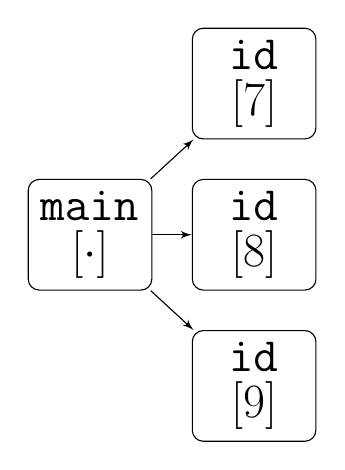
\begin{tikzpicture}
			\node [block] (main) {\LARGE{\tt main$_{}$}\\$[\cdot]$};
			\node [block, above right=0.5cm and 0.5cm of main] (id1) {\LARGE{\tt id$_{}$}\\$[7]$};
			\node [block, below = 0.5cm of id1] (id2) {\LARGE{\tt id$_{}$}\\ $[8]$};
			\node [block, below = 0.5cm of id2] (id3) {\LARGE{\tt id$_{}$}\\ $[9]$};
			
			\path [line] (main) -- (id1);
			\path [line] (main) -- (id2);
			\path [line] (main) -- (id3);
					
			\end{tikzpicture}
		}
	\end{center}
	\caption{Call-graph by 1-call-site sensitivity}
	\label{back:cfa:callgraph2}
\end{subfigure}
\qquad\linebreak\linebreak

\qquad
\begin{subfigure}[t]{0.9\columnwidth}
	\begin{center}
		\resizebox{0.4\columnwidth}{!}{
			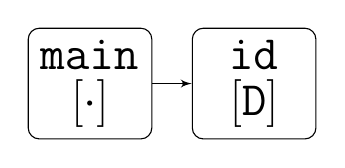
\begin{tikzpicture}
			\node [block] (main) {\LARGE{\tt main$_{}$}\\$[\cdot]$};
			\node [block, right = 0.5cm of main] (id) {\LARGE{\tt id$_{}$}\\${\tt[D]}$};
			
			\path [line] (main) -- (id);
			
			\end{tikzpicture}
		}
	\end{center}
	\caption{Call-graph by $k$-object sensitivity (for any $k$)}
	\label{back:obj:callgraph2}
\end{subfigure}
\end{multicols}
\vspace{-1em}
\caption{Typical situation that benefits from call-site sensitivity}
\label{back:b:Fig}
\vspace{-11pt}
\end{figure}




%%% Local Variables:
%%% mode: latex
%%% TeX-master: "paper"
%%% End:


\myparagraph{Benefit of Call-Site Sensitivity}
Figure~\ref{back:b:Fig} describes a typical situation where
call-site sensitivity has better precision than object sensitivity.
The example program has class {\tt D} that includes the identity
function {\tt id}. The {\tt main} method allocates an object of class
{\tt D} at line 6
and calls method {\tt id} on it in three places
at lines 7, 8, and 9 with different objects of type {\tt A}, {\tt B},
and {\tt C}, respectively.  Suppose pointer analysis aims to prove
that the three type-casting operations at lines 7, 8, and 9 are safe.
%(i.e. no down-casting violations occur).
Figure~\ref{back:cfa:callgraph2} shows the call-graph from
1-call-site-sensitive analysis. Note that the analysis analyzes the
method {\tt id} separately for the different call-sites at lines 
7, 8, and 9, and therefore is able to prove the safety of the queries. 


By contrast, $k$-object sensitivity is unable to prove any of the
queries in the program no matter what $k$ value is
used. Object sensitivity uses allocation-sites of receiver objects as
calling contexts. In this example, because the three method calls
share the same receiver object (i.e. the object pointed to by variable
{\tt d}), object sensitivity analyzes the method {\tt id}
with a single context element, namely the allocation-site {\tt D},
merging the three method calls (Figure~\ref{back:obj:callgraph2}).



\myparagraph{Benefit of Object Sensitivity}
Figure~\ref{back:a:Fig} %describes a major weakness of call-site sensitivity. 
describes a representative scenario where
object sensitivity is more precise than call-site sensitivity.
The example code in Figure~\ref{background:example1} has class {\tt C}
that contains $k+1$ methods
(${\tt id}_0, {\tt id}_1, \dots {\tt id}_k$), where each method
${\tt id}_i$ is semantically equivalent to the identity function
because ${\tt id}_0$ is the identity function and ${\tt id}_i$
%$(0< i \le k+1)$ 
{$(0< i \le k)$} calls ${\tt id}_{i-1}$ without modifying the formal
parameter {\tt v}.  The {\tt main} method has four heap allocation-sites:
namely, \texttt{C1}, \texttt{C2}, \texttt{A}, and \texttt{B}.  At line
13, {\tt main} calls ${\tt id}_k$ with the base variable {\tt c1} and
parameter \texttt{new A()}. At line {14}, ${\tt id}_k$ is called with
the base variable {\tt c2} and argument \texttt{new B()}.  Again, the goal
of pointer analysis is to prove the safety of the casting
operations at lines 13 and 14. For this program, a
$k$-call-site-sensitive analysis produces the call-graph in
Figure~\ref{back:cfa:callgraph}. Note that the method ${\tt id}_0$ is analyzed
under the single context ${[8,\dots,5]}$, where the critical information where
${\tt id}_k$ was originally called from is lost due to the truncation of
context strings to keep their last $k$ elements. 

Object sensitivity nicely addresses this shortcoming of call-site sensitivity. It uses the
allocation-sites, {\tt C1} and {\tt C2}, to represent the contexts of the
method calls to ${\tt id}_k$ at lines 13 and {14}, respectively. Note that the
receiver object remains the same in the subsequent calls to ${\tt id}_{k-1},
\dots {\tt id}_0$, propagating the initial contexts down to ${\tt id}_0$ and
producing the call-graph in Figure~\ref{back:obj:callgraph}. The
analysis is able to distinguish the two call chains and therefore proves the
queries.

%\textcolor{red}{Note that the shortcoming in handling nested method calls is the only weakness of call-site sensitivity; if there is no nested method call in a program, 1-call-site sensitivity becomes the most precise context abstraction. Suppose a program consists of methods that do not have any method call in their body except the main method. When analyzing the program, 1-call-site sensitivity will have the same precision with $\infty$-call-site sensitivity which is concrete context (the most precise context abstraction).}

% !TEX root = ./paper.tex

\begin{figure*}[t]	
\vspace{20pt}
\begin{multicols}{2}
\vfill\null
\begin{center}
\begin{subfigure}[b]{1.2\columnwidth}
\begin{lstlisting}[escapeinside={(*}{*)}, xleftmargin=12pt]
class C {
 Object id(*$_0$*)(v) {
  return v; }
 Object id(*$_1$*)(v) {
  return this.id(*$_{0}$*)(v); }
  ...
 Object id(*$_k$*)(v) {
  return this.id(*$_{k-1}$*)(v); }
}
main() {
 C c1 = new C();//C1
 C c2 = new C();//C2
 A a = (A)c1.id(*$_k$*)(new A());//A, query1
 B b = (B)c2.id(*$_k$*)(new B());//B, query2
}
\end{lstlisting}
\caption{Example code}
\label{background:example1}
\end{subfigure}
\end{center}
\columnbreak~\\~\\~\\
\vspace{-30pt}

%\scalefont{0.9}
%\qquad\qquad\qquad\qquad
%\begin{multicols}{3}
\begin{subfigure}[b]{0.9\columnwidth}
\begin{center}
				\resizebox{\columnwidth}{!}{
					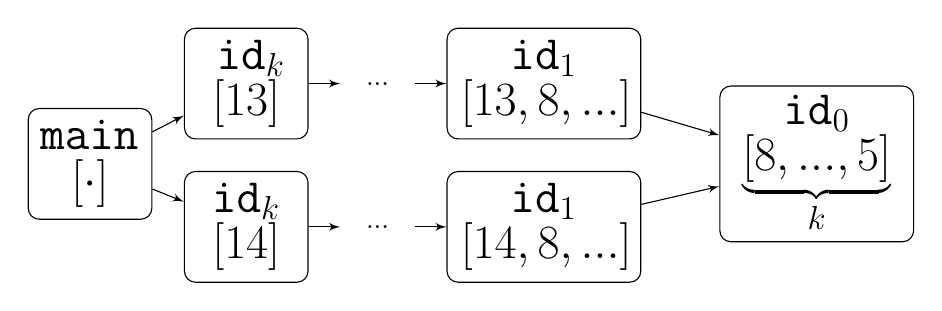
\begin{tikzpicture}
					\node [block] (main) {\LARGE{\tt main$_{}$}\\$[\cdot]$};
					\node [block, above right =
                                        -0.4cm and 0.4cm of main]
                                        (idk1) {\LARGE{ {\tt id}$_k$}\\$[13]$};
					\node [block, below = 0.4cm of idk1] (idk2) {\LARGE{\tt {id}$_k$}\\$[14]$};
					
					\node [onlyText, right=0.4cm of idk1] (dots1) {...};
					\node [onlyText, right=0.4cm of idk2] (dots2) {...};
					
					\node [block2, right=0.4cm of
                                        dots1] (id11) {\LARGE{\tt {id}$_1$}\\$[13,8,...]$};
					\node [block2, right=0.4cm of
                                        dots2] (id12) {\LARGE{\tt {id}$_1$}\\$[14,8,...]$};
					
					\node [block2, right = 7.2cm of
                                        main] (id0) {\LARGE{\tt id$_0$}\\$\underbrace{[8,...,5]}_k$};
					
					\path [line] (main) -- (idk1);
					\path [line] (main) -- (idk2);
					\path [line] (idk1) -- (dots1);
					\path [line] (idk2) -- (dots2);
					\path [line] (dots1) -- (id11);
					\path [line] (dots2) -- (id12);
					
					\path [line] (id11) -- (id0);
					\path [line] (id12) -- (id0);
					
					\end{tikzpicture}
				}
			\end{center}
			\vspace{-4pt}
			\caption{Call-graph by $k$-call-site sensitivity}
			\label{back:cfa:callgraph}
\end{subfigure} \vspace{8pt}
%	\vfill\null

%\qquad\qquad\qquad\qquad
\begin{subfigure}[b]{0.8\columnwidth}
\begin{center}
				\resizebox{\columnwidth}{!}{
					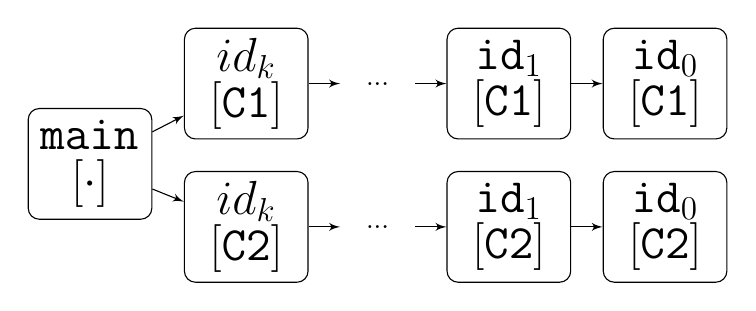
\begin{tikzpicture}
					\node [block] (main) {\LARGE{\tt main$_{}$}\\$[\cdot]$};
					\node [block, above right =
                                        -0.4cm and 0.4cm of main]
                                        (idk1) {\LARGE{\tt ${ id}_k$}\\${\tt [C1]}$};
					\node [block, below = 0.4cm of
                                        idk1] (idk2) {\LARGE{\tt ${ id}_k$}\\${\tt [C2]}$};
					
					\node [onlyText, right=0.4cm of idk1] (dots1) {...};
					\node [onlyText, right=0.4cm of idk2] (dots2) {...};
					
					\node [block, right=0.4cm of
                                        dots1] (id11) {\LARGE{\tt id$_1$}\\${\tt [C1]}$};
					\node [block, right=0.4cm of
                                        dots2] (id12) {\LARGE{\tt id$_1$}\\${\tt [C2]}$};
					
					\node [block, right=0.4cm of
                                        id11] (id01) {\LARGE{\tt id$_0$}\\${\tt [C1]}$};
					\node [block, right=0.4cm of
                                        id12] (id02) {\LARGE{\tt id$_0$}\\${\tt [C2]}$};
					
					\path [line] (main) -- (idk1);
					\path [line] (main) -- (idk2);
					\path [line] (idk1) -- (dots1);
					\path [line] (idk2) -- (dots2);
					\path [line] (dots1) -- (id11);
					\path [line] (dots2) -- (id12);
					
					\path [line] (id11) -- (id01);
					\path [line] (id12) -- (id02);
					
					\end{tikzpicture}
				}
			\end{center}
			\vspace{-4pt}
			\caption[]{Call-graph by 1-object sensitivity}
			\label{back:obj:callgraph}
\end{subfigure}
\vspace{8pt}
%	\vfill\null

%\qquad\qquad\qquad\qquad

\begin{subfigure}[b]{1.0\columnwidth}
	\begin{center}
				\resizebox{0.8\columnwidth}{!}{
					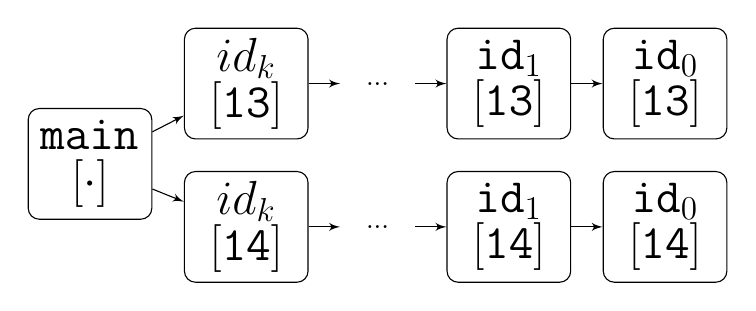
\begin{tikzpicture}
					\node [block] (main) {\LARGE{\tt main$_{}$}\\$[\cdot]$};
					\node [block, above right =
                                        -0.4cm and 0.4cm of main]
                                        (idk1) {\LARGE{\tt ${ id}_k$}\\${\tt [13]}$};
					\node [block, below = 0.4cm of
                                        idk1] (idk2) {\LARGE{\tt ${ id}_k$}\\${\tt [14]}$};
					
					\node [onlyText, right=0.4cm of idk1] (dots1) {...};
					\node [onlyText, right=0.4cm of idk2] (dots2) {...};
					
					\node [block, right=0.4cm of
                                        dots1] (id11) {\LARGE{\tt id$_1$}\\${\tt [13]}$};
					\node [block, right=0.4cm of
                                        dots2] (id12) {\LARGE{\tt id$_1$}\\${\tt [14]}$};
					
					\node [block, right=0.4cm of
                                        id11] (id01) {\LARGE{\tt id$_0$}\\${\tt [13]}$};
					\node [block, right=0.4cm of
                                        id12] (id02) {\LARGE{\tt id$_0$}\\${\tt [14]}$};
					
					\path [line] (main) -- (idk1);
					\path [line] (main) -- (idk2);
					\path [line] (idk1) -- (dots1);
					\path [line] (idk2) -- (dots2);
					\path [line] (dots1) -- (id11);
					\path [line] (dots2) -- (id12);
					
					\path [line] (id11) -- (id01);
					\path [line] (id12) -- (id02);
					
					\end{tikzpicture}
				}
			\end{center}
			\vspace{-4pt}
			\caption[]{1-call-site sensitivity with context tunneling}
			\label{back:callT:callgraph}
\end{subfigure}





\end{multicols}
%	\vfill\null
	%\columnbreak
% \begin{subfigure}[b]{0.5\columnwidth}
% \begin{center}
% 				\resizebox{\columnwidth}{!}{
% 					\begin{tikzpicture}
% 					\node [block] (main) {\Large{$\tt main_{}$}\\$[\cdot]$};
% 					\node [block, above right =
%                                         -0.4cm and 0.4cm of main]
%                                         (idk1) {\Large{\tt ${\tt id}_k$}\\$[13]$};
% 					\node [block, below = 0.4cm of idk1] (idk2) {{\tt $id_k$}\\$[14]$};
					
% 					\node [onlyText, right=0.4cm of idk1] (dots1) {...};
% 					\node [onlyText, right=0.4cm of idk2] (dots2) {...};
					
% 					\node [block, right=0.4cm of
%                                         dots1] (id11) {\Large{\tt ${\tt id}_1$}\\$[13]$};
% 					\node [block, right=0.4cm of
%                                         dots2] (id12) {\Large{\tt ${\tt id}_1$}\\$[14]$};
					
% 					\node [block, right=0.4cm of
%                                         id11] (id01) {\Large{\tt ${\tt id}_0$}\\$[13]$};
% 					\node [block, right=0.4cm of
%                                         id12] (id02) {\Large{\tt ${\tt id}_0$}\\$[14]$};
					
% 					\path [line] (main) -- (idk1);
% 					\path [line] (main) -- (idk2);
% 					\path [line] (idk1) -- (dots1);
% 					\path [line] (idk2) -- (dots2);
% 					\path [line] (dots1) -- (id11);
% 					\path [line] (dots2) -- (id12);
					
% 					\path [line] (id11) -- (id01);
% 					\path [line] (id12) -- (id02);
					
% 					\end{tikzpicture}
% 				}
% 			\end{center}
% 			\caption{Call-graph by 1-call-site-sensitivity
%                           with context tunneling}
% 			\label{back:callT:callgraph}
%  \end{subfigure}
%\vspace{-1em}
\vspace{-14pt}
	\caption{Typical situation that benefits from object sensitivity}
	\label{back:a:Fig}
\vspace{-10pt}
\end{figure*}


%%% Local Variables:
%%% mode: latex
%%% TeX-master: "paper"
%%% End:



\myparagraph{Known Superiority} 
 Though call-site sensitivity and object sensitivity have their own
 strengths and weaknesses, object
  sensitivity is widely known to be superior to call-site sensitivity 
  because real-world programs involve code patterns such as one in
  Figure~\ref{back:a:Fig} more often. 
  Note that the existing superiority holds empirically, rather than theoretically, based on the experimental results of prior work~(e.g., \cite{Lhotak2008,BravenboerS09}).  
  

%\textcolor{red}{
%Though call-site sensitivity and object sensitivity have their own
%strengths and weaknesses, object sensitivity has been known to be
%superior to call-site sensitivity based on prior works' empirical evaluation
%result~\cite{Lhotak2008,BravenboerS09}.  
%Object sensitivity has shown a better performance than call-site
%sensitivity because real-world object-oriented programs involve code
%patterns such as one in Figure~\ref{back:a:Fig} more often. 
%}


%\vspace{-20pt}
\subsection{Revisiting the Superiority in Generalized $k$-Limited Setting}\label{sec:overview-result}
%\noindent
Our new claim is that the known superiority of object sensitivity over call-site sensitivity no longer holds when the notion of $k$-limiting is generalized with context tunneling. 

%In this paper, we show that 
%the existing 
%superiority of object sensitivity over call-site sensitivity holds only in the traditional $k$-limited setting, where the
%analysis is enforced to keep the most recent $k$ context elements, but no longer holds in a more general setting with context tunneling. 

\myparagraph{Context Tunneling}
Context tunneling~\cite{JeJeOh18} allows an analysis to maintain an arbitrary $k$-length subsequence of context strings.
For example, when $s = [C_1, C_2, C_3, C_4, C_5]$ is a sequence of
context elements that may appear in an unbounded ($k=\infty$)
context-sensitive analysis, the traditional $3$-limited analysis
abstracts the context string into its suffix $[C_3,C_4,C_5]$. 
With context tunneling, however, the analysis is free to use any
subsequence of $s$ such as $[C_1, C_3, C_5]$ and $[C_2, C_4, C_5]$, as
a $k$-limited abstraction of the original context string. 
Note that the traditional $k$-limited approach is a special case of the
generalized approach with context tunneling. 


\myparagraph{Key Insight}
Our key insight is summarized as follows: 
%that call-site sensitivity is superior to
%object sensitivity when they are generalized
%with context tunneling: 
\begin{itemize}[leftmargin=1.3em]
\item The major weakness of call-site sensitivity
in the traditional setting is no longer a weakness in the generalized
$k$-limited setting with context tunneling.%~\minseok{conflict. Need revision??} 
\item By contrast, object sensitivity still suffers from its
limitation even with the generalization. 
\end{itemize}

%For example, 
With context tunneling, call-site sensitivity does not
suffer from its shortcoming and can now prove the queries in
Figure~\ref{background:example1}. Suppose that we use a
context-tunneling policy that chooses the first $k$ elements of a
context string rather than the last $k$ ones.
%\textcolor{red}{Context tunneling achieves this by selectively updating contexts. 
%When {\tt id$_i$} (i<k) is called, the context-tunneling policy makes the callee method inherit the context of the caller method instead of updating context with the invocation site.} 
Then, the resulting
1-call-site-sensitive analysis produces the call-graph in Figure~\ref{back:callT:callgraph},
which is exactly the same as the
call-graph of the 1-object-sensitive analysis in
Figure~\ref{back:obj:callgraph}. Because the call-graphs are
equivalent, the call-site-sensitive analysis is as precise as the
object-sensitive analysis, successfully proving the queries. 



On the other hand, object sensitivity fails to simulate call-site
sensitivity even with context tunneling.  Consider the program in
Figure~\ref{back:b:Fig} where call-site sensitivity is
typically more precise than object sensitivity. For this program,
object sensitivity cannot prove all of the queries no matter what
context-tunneling policy and $k$ value are used. 
%\minseok{$k$-object-sensitivity with context tunneling can prove only one query among them.}
In
Figure~\ref{back:b:Fig}, object sensitivity can use the
allocation-site {\tt D} as context elements. Thus, only the two
context subsequences, i.e., \texttt{[D]} and \texttt{[$\cdot$]}, are
possible for the method {\tt id} with context tunneling, all of which
fail to analyze {\tt id} separately for the three different
call-sites.  % In this sense, object sensitivity is 
% inevitably less precise than call-site sensitivity in the generalized $k$-limited setting. 

%\myparagraph{Incompleteness}

We clarify that, like the previously known superiority, our claim in this paper is empirical. 
On the theoretical side, we do not know yet whether or not call-site sensitivity can always simulate object sensitivity in the general setting with context tunneling, which we leave as an open question for future work. We discuss this issue in more detail in Section~\ref{sec:counter_example}.
%not theoretical.  
%We can construct a counter-example such that
%context-tunneled call-site sensitivity is unable to simulate object
%sensitivity (Section~\ref{sec:counter_example}).  
%However,  such a counter-example is uncommon in practice, allowing the simulation to be almost complete for real-world programs. 
%(Sections \RNum{1} and \RNum{2} of the supplementary
%material and Section~\ref{sec:eval_learning}).


\myparagraph{\ourtechnique}
Based on the insight, 
%To support the claim, 
we develop \ourtechnique, a practical technique for transforming a given $k$-object-sensitive analysis 
into a more precise, context-tunneled $k$-call-site-sensitive analysis (Section~\ref{sec:technique}).  The
resulting analysis is (empirically) more precise than the baseline
object sensitivity, as it enjoys the benefits of both object
sensitivity and call-site sensitivity. For example, it
produces precise results for both cases in Figure~\ref{back:b:Fig} and~\ref{back:a:Fig}.


%%% Local Variables:
%%% mode: latex
%%% TeX-master: "paper"
%%% End:

%\input{analysis}
% !TEX root = ./paper.tex

\chapter{Is Complete Simulation Possible?}\label{sec:appendix}
% In this thesis, we showed that it is practically possible to outperform object sensitivity via context-tunneled call-site sensitivity (Chapter~\ref{sec:Obj2CFA}). 
% However, it remains to be seen whether or not call-site sensitivity can be fundamentally superior to object sensitivity.
Before we introduce the formal description the fundamental superiority, we redefine pointer analysis with tunneling on which the formal description will be simply defined. Note that the analysis below is fundamentally the same analysis used in Chapter~\ref{sec:Preliminaries},~\ref{sec:Tunneling}, \ref{sec:Obj2CFA}, and \ref{sec:Graphick}.

%In this section, we define a pointer analysis with context tunneling. 


%\subsection{Context-Tunneled Pointer Analysis}
\label{sec:pointeranalysis}


\myparagraph{Program}
We assume a program is a sequence of instructions, where each
instruction is associated with a distinct label.  An instruction is
either heap allocation (${\it x = new()}$), move (${\it x = y}$), 
%\textcolor{red}{
store (${\it x.f = y}$), load (${\it x = y.f}$),
%}
or
virtual method call (${\it x = y.m_r^{p}(a)}$).  We
assume that every method ($m$) has a single formal parameter ($p$) and
return variable ($r$). 
Given a program $P$ to analyze, we assume the following:
\begin{itemize}[leftmargin=1.4em]
\item $\Var_P$: the set of program variables.
\item $\fld_P$: the set of field signatures.
\item $\Inst_P$: the set of instruction labels of the program.
\item $\Methods_P$: the set of methods of the program.
\item $\mthdof_P$: the mapping from labels to the
methods containing them (i.e. $\Inst_P \to \Methods_P$).
\item $\Invo_P$: invocation sites (i.e. call sites, $\Invo_P \subseteq \Inst_P$).
\item $\Heap_P$: heap allocation sites (i.e. $\Heap_P \subseteq \Inst_P$).
\item $\Ctx_P$: the set of calling contexts (i.e. $\Ctx_P = \Inst_P^*$).
\item $\Hctx_P$: the set of heap contexts (i.e. $\Hctx_P = \Inst_P^*$).
\item $\entry_P$: the entry method of the program.
\end{itemize}


\myparagraph{Notation}
For function $X: A \to B$, where $A$ and $B$ are sets, we write $X[a
\mapsto b]$ %\begin{comment}
(where $a \in A, b \in B$)
%\end{comment}
for the function $X$ that is extended to map  $a$ to $b$.
For function $X: A \to \power{B}$,
$X[ a \weakupdate b]$ 
%\begin{comment}
(where $a \in A, b \subseteq B$)
%\end{comment} 
denotes $X[ a\mapsto X(a) \cup b]$ (i.e. weak update).
Given $X, Y: A \to \power{B}$, $X \sqcup Y$ denotes $\lambda
a. X(a) \cup Y(a)$. Given a sequence $s = a_1a_2\dots a_{n-1}$ and an element
$a_n$, we write $\truncateCtx{s \concat a_n}{k}$ for $a_1a_2\dots a_{n-1}a_n$
if $n < k$. If $n \ge k$, the result is $a_{n-k+1} \dots a_{n-1}a_n$.


%\myparagraph{Tunneling Abstraction}
\myparagraph{Pointer Analysis} % with Context Tunneling}
%The idea of context tunneling~\cite{JeJeOh18} is to selectively update contexts. 
%To support context tunneling, we parameterize a pointer analysis by a tunneling abstraction, $T$, which is a set of invocation sites.  
%
%\begin{comment}
%For example, when
%$k=1$,  a caller method $m_{1}$ with context
%$[i_{1}]$ calls a method $m_{2}$ at call-site $i_{2}$, and
%$i_2 \in T$, the context of the callee $m_2$ inherits the caller's
%and becomes $[i_{1}]$, not $[i_{2}]$.  
%
%When $T =
%\emptyset$, we do not apply context tunneling at all, so the analysis
%becomes the conventional
%$k$-context-sensitive analysis. % that keeps the last
%% $k$ context elements.
%When $T =
%\Invo_P$, on the other hand, the analysis becomes context-insensitive
%because every call-site is tunneled and therefore all the
%methods are analyzed under the initial context of the entry method.
%%\end{comment}
%
%
%
%\myparagraph{Analysis Rules} 
We consider a subset-based pointer analysis with on-the-fly call-graph construction~\cite{Smaragdakis2015}, which computes four pieces of
information: points-to, field points-to, reachability, and call-graph
information. The points-to information,
$\ptsto\in \Var_P \times \Ctx_P \to \power{\Heap_P \times \Hctx_P}$, maps
variables with contexts to sets of heaps with heap contexts.  
The field points-to information,
$\fptsto \in \Heap_P \times \Hctx_P \times \fld_P \to \power{\Heap_P \times \Hctx_P}$, maps
fields of heaps with their heap contexts to sets of heaps with heap contexts.  
The
reachability information, $\reachable \in \Methods \to \power{\Ctx}$,
maps methods to their reachable contexts. 
A call-graph,
$\callgraph\in \power{\Invo_P \times \Ctx_P\times \Methods_P\times \Ctx_P}$,
is a set of context-sensitive call edges, where
$(\invo,\ctx_1,m,\ctx_2) \in \callgraph$ indicates that method $m$ is
called from the invocation-site $\invo$ and the caller and callee
contexts are $\ctx_1$ and $\ctx_2$, respectively. The analysis is
flow-insensitive and aims to compute the least fixed point of the semantic function $F$ defined as follows:
\[
F^{T,U}_{P,k} = \lambda (\ptsto, \fptsto, \reachable, \callgraph). \bigsqcup_{\inst \in \Inst_P}
f^{T, U}_{\inst, k}(\ptsto, \fptsto ,\reachable, \callgraph) 
\]
where $k \in \mbn$ is the maximum context depth to distinguish and  $f^{T, U}_{\inst, k}$ is the transfer function for the instruction whose label is $\inst$. $T$ and $U$ are context-tunneling abstraction and context-update function, respectively, which will be explained shortly. Running the analysis is to compute $\fix F$:
\[
\fix F^{T,U}_{P,k} = F^{T,U}_{P,k} (\bot_X, \bot_Y, \bot_R, \bot_G) \sqcup F^{T,U}_{P,k} (F^{T,U}_{P,k} (\bot_X, \bot_Y, \bot_R, \bot_G)) \sqcup \dots
\]
where the bottom elements are defined as follows:
\[
  \bot_\ptsto = \lambda (x,c).\emptyset, \qquad   \bot_\fptsto = \lambda (l,hc,f).\emptyset, \qquad \bot_\reachable =
\lambda m. \left\{ \begin{array}{ll} \myset{\epsilon} & \mbox{if}~m =
                                                        \entry_P \\
                     \emptyset & \mbox{otherwise} \end{array} \right., \qquad
  \bot_\callgraph = \emptyset.
\]


\myparagraph{Transfer Function}
The transfer function for the allocation, move, store, and load instructions is standard.
Let $(\ptsto', \fptsto', \reachable',\callgraph')$ be $f^{T, U}_{\inst, k}(\ptsto, \fptsto,\reachable,\callgraph)$. 
When the command is allocation ({\it x
  = new()}), it extends the points-to map so that the variable {\it x}
points-to the heap $\inst$ under the reachable context $\ctx \in \reachable(\mthdof(l))$: 
\[
\vspace{-0.3em}
%\begin{array}{c}
\ptsto' = \bigsqcup_{\ctx \in \reachable(\mthdof(l))} \ptsto [ (x,
\ctx)\weakupdate \myset{(l, \ctx)} ].
%\end{array}
\]
For a store command 
({\it ${\it x.f = y}$}), the field points-to information is updated as follows:
\[
\vspace{-0.3em}
%\begin{array}{c}
\fptsto' = \bigsqcup_{\ctx \in \reachable(\mthdof(l))} \fptsto [(l,
\hctx,f)\weakupdate \myset{(l', \hctx')} ]
%\end{array}
\]
where $(l,hctx) \in \ptsto(x,ctx)$ and $(l',\hctx') \in
X(y,\ctx)$. The points-to information is updated as follows for a
load (${\it x = y.f}$) instruction: 
\[
\vspace{-0.3em}
%\begin{array}{c}
\ptsto' = \bigsqcup_{\ctx \in \reachable(\mthdof(l))} \ptsto [(x,
\ctx)\weakupdate \myset{(l, \hctx)}]
%\end{array}
\]
where $(l,\hctx) \in \fptsto(l',\hctx',f)$ and $(l',\hctx') \in X(y,\ctx)$.
The reachability map and call-graph remain the same for the above instructions (i.e. $\reachable'=\reachable$ and $\callgraph'=\callgraph$). 
The transfer function for move instruction ($\it x = y$) combines the points-to set of
${\it y}$ into that of ${\it x}$ without modifying $\reachable$ and $\callgraph$.
%\[
%\ptsto' = \bigsqcup_{\ctx \in \reachable(\mthdof(l))} \ptsto[(x, \ctx) \weakupdate \ptsto(y,
%                 \ctx)].
%\]

The transfer function for method calls is less standard as it should 
account for context tunneling. 
To support context tunneling~\cite{JeJeOh18}, we assume a context-tunneling space $\mbs$ is given. 
The space $\mbs$ can be defined in various ways and the choice does not affect the soundness of the analysis. 
In this chapter, we simply define the space to be the set of all invocation sites, i.e., $\mbs = \Invo_P$ and let $T \subseteq \mbs$ be a tunneling abstraction given before the analysis. 
For method call ${\it x =
y.m^p_r(a)}$, 
the transfer function, $f^{T, U}_{\inst, k}$,  first generates the callee's context $\ctx'$ using the context-update function $\updatectx$, $\ctx' = \updatectx(\ctx, T, X, l, y, k)$, which takes information available at the
call-site. 
The output $\ctx'$ of $\updatectx$ will be shortly defined for each context sensitivity flavor.
Once $\ctx'$ is computed, the analysis makes the formal
parameter $p$ under $\ctx'$ have the points-to set of the actual
parameter $a$ under $\ctx$ and the points-to set of the return variable
$r$ is transferred to the variable
$x$. The resulting $\ptsto'$ is
defined as follows: 
\[
 \bigsqcup_{\ctx \in \reachable(\mthdof(l))}
  	\ptsto[	(p,\ctx')
	\weakupdate \ptsto(a, \ctx), 
	(x, \ctx) \weakupdate \ptsto(r,
	\ctx')]
\]
     and the reachability and call-graph are updated accordingly:
      $\reachable' = \reachable[ m \weakupdate \myset{\ctx'}]$ and $\callgraph' = \callgraph \cup\{(\inst,ctx,m,ctx')\}$.


%the analysis generate
%callee method's context and weak updates 

%When the instruction at $\inst$ is ${\it x =
%y.m^p_r(a)}$, $f_{k,i}^{T,
%\updatectx}(\ptsto,\reachable, \callgraph)$ takes care of parameter and return
%value passing, producing the following:
%\[
%\begin{array}{rr}
%\bigsqcup\limits_{\ctx \in \reachable(\mthdof(l))}
%\myset{(
%\ptsto
%\left[
%\begin{array}{l}
%             (p,\ctx')
%  \weakupdate \ptsto(a, \ctx), \\
%  (x, \ctx) \weakupdate \ptsto(r,
%  \ctx')
%\end{array}
%  \right], \reachable[ m \weakupdate \myset{\ctx'}],
%  \\\callgraph \cup\{(\inst,ctx,m,ctx')\})
%  \mid \ctx'=\updatectx^{k, T}(\ctx, X, l, y)}.
%\end{array}
%\]
%From the context $\ctx$, we first generate the callee's context
%$\ctx'$ using $\updatectx$, which takes information available at the
%call-site and produces new contexts (details to be explained shortly). Then, the analysis makes the formal
%parameter $p$ under $\ctx'$ have the points-to set of the actual
%parameter $a$ under $\ctx$. The points-to set of the return variable
%$r$ is transferred to the variable $x$. 
%%\end{itemize}

%\subsection{Context Tunneling}\label{sec:tunneling}
%
%We now define object sensitivity and call-site sensitivity with context tunneling. 

\myparagraph{Context Update}
Let us define the context-update function $\updatectx$. 
For object sensitivity, it is defined as follows: 
\begin{equation}\label{eq:objsens}
\begin{array}{rr}
\updatectx (\ctx, T, X, l, y, k) =
\left\{
\begin{array}{ll}
\truncateCtx{\hctx \concat h}{k} & l \not\in T, \\
\hctx & l \in T
\end{array}
\right.\\
\end{array}
\end{equation}
where $(h, \hctx) \in X(y, \ctx)$.
When a method is called from an
      invocation site $l$ with the base variable $y$ and caller's
      context $\ctx$, the analysis first looks at the heap $h$ (and
      its context $\hctx$) that the variable $y$ under $\ctx$ points
      to, and creates the callee's context by appending the heap ($h$)
      to its heap context ($\hctx$). The context may be truncated to
      keep the last $k$ elements at most (i.e.
      $\truncateCtx{\hctx \concat h}{k}$).
Note that 
$\updatectx$ creates the new context only when $l \not\in
T$ (i.e. no context tunneling). Otherwise ($l \in T$), it applies context tunneling and propagates the existing 
context ($\hctx$). 

%By combining the information, 
%The definition of $\updatectx$ for object-sensitivity~\cite{Milanova2005,Smaragdakis2011}
%is defined as follows:
% produces the callee's context.
%For instance, object-sensitivity~\cite{Milanova2005,Smaragdakis2011} can be specified
%by defining $\updatectx$ as follows:
%

%\paragraph{Call-Site Sensitivity}
For call-site sensitivity, $\updatectx$ is defined as follows: 
\begin{equation}\label{eq:cfa}
\updatectx(\ctx, T, X, l, y, k) =
    \left\{
      \begin{array}{ll}
        \truncateCtx{\ctx \concat l}{k} & l \not\in T, \\
        \ctx & l \in T
      \end{array}
    \right.
\end{equation}
When $l \not\in T$, 
%When a method is called at an invocation site $l$ in a method under the context
%$\ctx$, 
the analysis appends 
the current invocation site $l$ to
$\ctx$. With context tunneling ($l \in T$), it uses the caller's context $\ctx$ for the callee's. 



%\textcolor{red}{
%Note that we can define the abstraction space of context tunneling in various ways.
%In this paper, we use the set of invocation sites as an abstraction space; a tunneling abstraction determines whether to update contexts with method invocation sites. 
%In the previous work~\cite{JeJeOh18}, on the other hand, the space of tunneling is defined with methods; a tunneling abstraction determines whether to apply tunneling with methods.
%}

% \myparagraph{Instance Analyses}
% Given  a program $P$ and 
% its tunneling abstraction $T \subseteq \Invo_P$, 
% we write $\call_k(P, T)$ and
% $\obj_k(P, T)$ for the $k$-call-site- and
% $k$-object-sensitive analyses, respectively. In the rest of the paper, we fix $k$ and omit the subscript $k$ from $\call_k$ and $\obj_k$. 
% These instance analyses are used with a {\em context-tunneling policy}. 
% A context-tunneling policy $\heuristic$ is a function that maps a program $P$ into
% a tunneling abstraction for $P$: 
% \[
%   \heuristic(P) \subseteq \Invo_P.
% \]
% With a policy $\heuristic$, 
% we  perform the analysis for a program $P$ as follows: $\call(P, \heuristic(P))$ or $\obj(P, \heuristic(P))$. 

 % which first uses $\heuristic$ to produce a tunneling abstraction $\heuristic(P)$ and analyzes the program with the abstraction. 

%%% Local Variables:
%%% mode: latex
%%% TeX-master: "paper"
%%% End:

% !TEX root = ./paper.tex

%\input{analysis}


\section{\ourtechnique: Transforming Object Sensitivity to Call-Site Sensitivity}\label{sec:technique}
We now present our technique, \ourtechnique. 
Given an object-sensitive analysis specified by an arbitrary
tunneling policy $\objheuristic$, our technique transforms it to another
tunneling policy $\callheuristic$
%\[
%\objheuristic \to \mbox{\ourtechnique} \to \callheuristic
%\]
such that the
call-site-sensitive analysis with $\callheuristic$ becomes more precise
than the baseline object-sensitive analysis with $\objheuristic$. 

To achieve this, \ourtechnique~works in the two steps: simulation and learning. 
It first converts $\objheuristic$ into
a {\em simulated policy} $\simheuristic$. 
%\[
%    \objheuristic \to \mbox{Simulation} \to \simheuristic
%\]
With $\simheuristic$, call-site sensitivity becomes
more precise than object sensitivity with $\objheuristic$
but running the analysis with $\simheuristic$
is expensive as it uses the baseline
object-sensitive analysis as a pre-analysis. 
The purpose of the second step is to  remove this overhead
 by learning the behavior of $\simheuristic$ from training data.  
%\[
%  \begin{array}{r}
%%    \simheuristic \to\\[0.1em]
%   \simheuristic +  \mbox{training data} \to
%  \end{array}
%  \mbox{Learning} \to \callheuristic \qquad\qquad
%\]
The learned policy $\callheuristic$ is as precise as
$\simheuristic$ but more efficient as it does not rely on the
simulation procedure. 






%%% Local Variables:
%%% mode: latex
%%% TeX-master: "paper"
%%% End:

% !TEX root = ./paper.tex


\subsection{Simulation}\label{sec:simulation}

%A key insight behind our technique is that call-site sensitivity with
%context tunneling can simulate object sensitivity.  That is, 

The first technical contribution of this chapter is the simulation procedure. 
Given a program $P$ and its tunneling abstraction $\Tobj \subseteq \mbi_P$, where $\Tobj$ is given by $\objheuristic$, i.e., 
$\Tobj = \objheuristic(P)$,
the goal of simulation is to infer a tunneling abstraction
$\Tcall \subseteq \mbi_P$ such that $\call(P, \Tcall)$ becomes more
precise than $\obj (P, \Tobj)$.


% !TEX root = ../thesis.tex


%basicstyle=\linespread{1.2}\small\ttfamily
\begin{figure}[t]
%\setlength{\columnsep}{0.07cm}
\begin{lstlisting}[multicols=2, escapeinside={(*}{*)},xleftmargin=4.0ex ,basicstyle={\linespread{1.2}\fontsize{9.5}{10}\selectfont\ttfamily}]
class D {
 Object id(v) {
  return v;}
 Object id1(v) {
  return this.id(v);}
 void m() {
  A a = (A)this.id(new A());//A1, qry1
  B b = (B)this.id(new B());//B1, qry2
 }
}
void main() {
 D d1 = new D();//D1
 D d2 = new D();//D2
 D d3 = new D();//D3 

 A a3 = (A)d1.id1(new A());//A2, qry3 
 B b3 = (B)d2.id1(new B());//B2, qry4
 d3.m();
}
\end{lstlisting}
%\vspace{-15pt}
\caption{Running example}
%\vspace{-15pt}
\label{simulation:example}
\end{figure}


%%% Local Variables:
%%% mode: latex
%%% TeX-master: "../thesis.tex"
%%% End:


\myparagraph{Running Example}
\label{sec:simulation-overview}
We illustrate the simulation procedure with the
example program in Figure~\ref{simulation:example}.  The code
contains class {\tt D} that has three methods \texttt{id},
\texttt{id1}, and \texttt{m}.  Methods \texttt{id} and \texttt{id1}
are identity functions.
The method \texttt{m} contains two method invocations at lines 7 and
8, which call \texttt{id} with new \texttt{A} and \texttt{B} objects.
The \texttt{main} method creates three objects at the
allocation-sites \texttt{D1}, \texttt{D2}, and \texttt{D3}, and stores
them in variables \texttt{d1}, \texttt{d2} and \texttt{d3},
respectively.  At line 16, \texttt{main} calls \texttt{id1} with
a new object of type {\tt A} and the base variable \texttt{d1}.  At line 17,
\texttt{id1} is called with a new object with type {\tt B} and base variable
\texttt{d2}.  At line 18, \texttt{main} also calls {\tt m} with base
variable \texttt{d3}.  We assume that the code has four queries, which ask the
safety of casting operations at lines 7, 8, 16, and 17. Note that all
of these are safe since {\tt id} and {\tt id1} are identity
functions.








In this example, for simplicity, we assume an 1-object-sensitive analysis
without context tunneling (i.e. $\Tobj = \emptyset$) is given but our technique is applicable
to object sensitivity with arbitrary $k$ and tunneling abstraction $\Tobj \subseteq \mbi_P$. 
Figure~\ref{fig:obj:callgraph} shows the call-graph produced by the
baseline 1-object-senstivie analysis, 
where a call-graph edge is represented by invocation-site, caller method, caller context, 
callee method, and callee context. For example, the edge
$\texttt{id1[D1]} \stackrel{5}{\to} \texttt{id[D1]}$ indicates that
method {\tt id} is called from {\tt id1} at invocation-site $5$,
where the callee and caller contexts are {\tt D1}.  Note that
this object-sensitive analysis is not precise enough to prove all queries.
Although it can prove queries at lines 16 and
17 as it distinguishes the two different contexts of {\tt id1}, it
fails to prove queries at lines 7 and 8 because it uses the same
context {\tt [D3]} for {\tt id} at both call-sites.





%\begin{comment}
%\textcolor{blue}{
Figure~\ref{fig:CFA:callgraph} shows the call-graph obtained by the
ordinary 1-call-site-sensitive analysis without context tunneling. 
Note that the precision of the analysis is incomparable to
that of the baseline 1-object sensitivity. 
Because the analysis uses the
call-site as the calling context, it is able to prove
the queries at
lines 7 and 8 by separately analyzing the two calls to \texttt{id}. However,
it fails to prove the queries at lines
16 and 17 as the variable {\tt v} in \texttt{id} under context
\texttt{[5]} points-to both heap objects \texttt{A2} and \texttt{B2}
that in turn
propagates back to the variables {\tt a} and {\tt b} in the
\texttt{main} method.
%}
%\end{comment}


% !TEX root = ./paper.tex



\begin{figure*}[t]
	\begin{multicols}{4}
		\begin{subfigure}[b]{1.\columnwidth}
			\begin{center}
				\resizebox{1.\columnwidth}{!}{
					\tikzstyle{every node}=[font=\LARGE]
					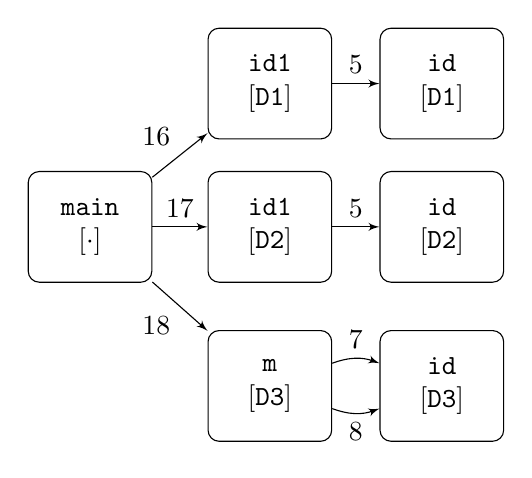
\begin{tikzpicture}
					\node [block] (main) {{\tt main}\\$[\cdot]$};
					\node [block, right = 0.7cm of main] (id11) {\tt {id1}\\$[$D2$]$};
					\node [block, above = 0.4cm of id11] (id12) {\tt {id1}\\$[$D1$]$};
					
					\node [block, right=0.6cm of id11] (oid1) {\tt {id}\\$[$D2$]$};
					\node [block, right=0.6cm of id12] (oid2) {\tt {id}\\$[$D1$]$};
					
					\node [block, below = 0.6cm of id11] (m) {\tt {m}\\$[$D3$]$};
					
					\node [block, right=0.6cm of m] (nid) {\tt {id}\\$[$D3$]$};
					
					\path [line] (main) edge node[above] {17} (id11);
					\path [line] (main) edge node[above left] {16} (id12);
					\path [line] (id11) edge node[above] {5} (oid1);
					\path [line] (id12) edge node[above] {5} (oid2);
					\path [line] (main) edge node[below left] {18} (m);
					\path [line] (m) edge [bend left=20] node[above] {7} (nid);
					\path [line] (m) edge [bend right=20] node[below] {8} (nid);
					\end{tikzpicture}
				}
			\end{center}
			\vspace{7pt}
			~\\
			\caption{\small $1$-object sensitivity with $\Tobj = \emptyset$}
			\label{fig:obj:callgraph}
		\end{subfigure}
		\vfill\null
		\columnbreak
		\begin{subfigure}[b]{1\columnwidth}
			\begin{center}
				\resizebox{1\columnwidth}{!}{
					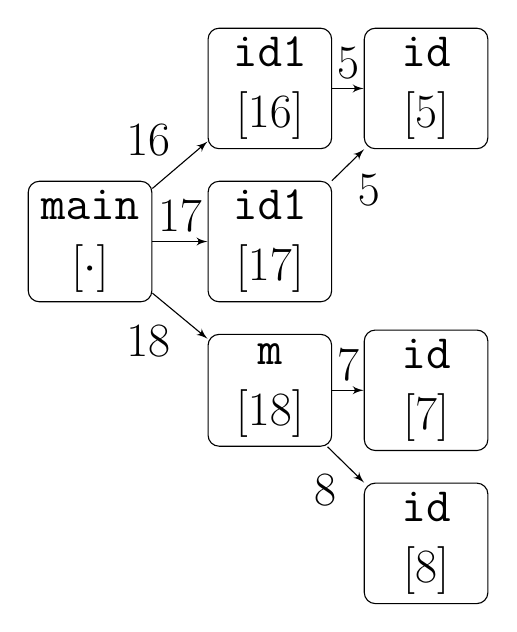
\begin{tikzpicture}
					\tikzstyle{every node}=[font=\LARGE]				
					\node [block] (main) {\tt {main}\\$[\cdot]$};
					\node [block, right = 0.7cm of main] (id11) {\tt {id1}\\$[17]$};
					\node [block, above = 0.4cm of id11] (id12) {\tt {id1}\\$[16]$};
					
					%\node [block, right = 0.4cm of id11] (oid1) {{\tt id}\\$[17]$};
					\node [block, right = 0.4cm of id12] (oid2) {\tt {id}\\$[5]$};
					
					\node [block, below = 0.4cm of id11] (m) {\tt {m}\\$[18]$};
					
					\node [block, right=0.4cm of m] (nid1) {\tt {id}\\$[7]$};
					\node [block, below=0.4cm of nid1] (nid2) {\tt {id}\\$[8]$};
					
					
					\path [line] (main) edge node[above] {$17$} (id11);
					\path [line] (main) edge node[above left] {$16$} (id12);
					\path [line] (id11) edge node[below right] {$5$} (oid2);
					\path [line] (id12) edge node[above] {$5$} (oid2);
					\path [line] (main) edge node[below left] {$18$} (m);
					\path [line] (m) edge node[above] {$7$} (nid1);
					\path [line] (m) edge node[below left] {$8$} (nid2);				
					\end{tikzpicture}
				}
			\end{center}
			\vspace{5pt}
			\caption{\small $1$-CFA with $\Tcall = \emptyset$}
			\label{fig:CFA:callgraph}
		\end{subfigure}
		\vfill\null
		\columnbreak
		\begin{subfigure}[b]{1\columnwidth}
			\begin{center}
				\resizebox{1\columnwidth}{!}{
					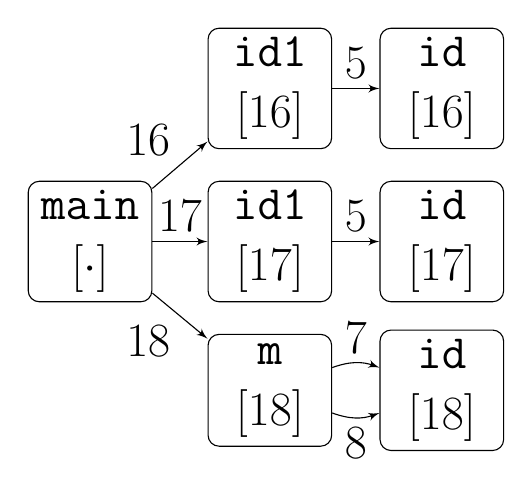
\begin{tikzpicture}
					\tikzstyle{every node}=[font=\LARGE]
					\node [block] (main) {\tt {main}\\$[\cdot]$};
					\node [block, right = 0.7cm of main] (id11) {\tt {id1}\\$[17]$};
					\node [block, above = 0.4cm of id11] (id12) {\tt {id1}\\$[16]$};
					
					\node [block, right=0.6cm of id11] (oid1) {\tt {id}\\$[17]$};
					\node [block, right=0.6cm of id12] (oid2) {\tt {id}\\$[16]$};
					
					\node [block, below = 0.4cm of id11] (m) {\tt {m}\\$[18]$};
					
					\node [block, right=0.6cm of m] (nid) {\tt {id}\\$[18]$};
					
					
					\path [line] (main) edge node[above] {$17$} (id11);
					\path [line] (main) edge node[above left] {$16$} (id12);
					\path [line] (id11) edge node[above] {$5$} (oid1);
					\path [line] (id12) edge node[above] {$5$} (oid2);
					\path [line] (main) edge node[below left] {$18$} (m);
					\path [line] (m) edge [bend left=20]  node[above] {$7$} (nid);
					\path [line] (m) edge [bend right=20]  node[below] {$8$} (nid);
					
					\end{tikzpicture}
				}			
			\end{center}
			%\vspace{-10pt}
			~\\
			\vspace{9pt}
			\caption{\small $1$-CFA with $\Tcall = \myset{5,7,8}$}
			\label{fig:call:callgraph}
		\end{subfigure}
		\vfill\null
		\columnbreak
		\begin{subfigure}[b]{1\columnwidth}
			\begin{center}
				\resizebox{1\columnwidth}{!}{
					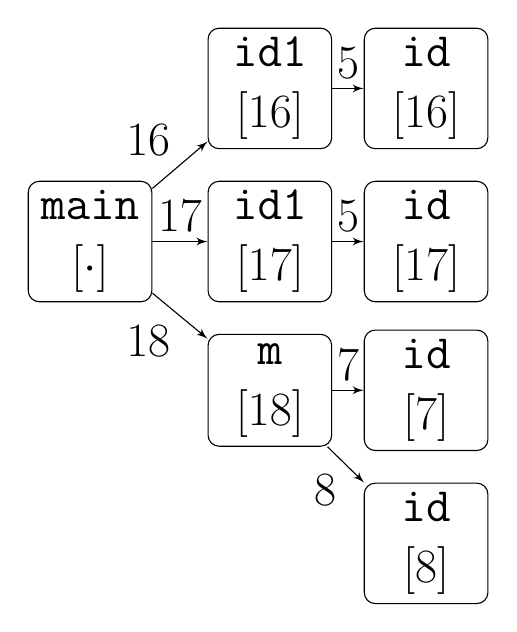
\begin{tikzpicture}
					\tikzstyle{every node}=[font=\LARGE]
					\node [block] (main) {\tt {main}\\$[\cdot]$};
					\node [block, right = 0.7cm of main] (id11) {\tt {id1}\\$[17]$};
					\node [block, above = 0.4cm of id11] (id12) {\tt {id1}\\$[16]$};
					
					\node [block, right=0.4cm of id11] (oid1) {\tt {id}\\$[17]$};
					\node [block, right=0.4cm of id12] (oid2) {\tt {id}\\$[16]$};
					
					\node [block, below = 0.4cm of id11] (m) {\tt {m}\\$[18]$};
					
					\node [block, right=0.4cm of m] (nid1) {\tt {id}\\$[7]$};
					\node [block, below=0.4cm of nid1] (nid2) {\tt {id}\\$[8]$};
					
					
					\path [line] (main) edge node[above] {$17$} (id11);
					\path [line] (main) edge node[above left] {$16$} (id12);
					\path [line] (id11) edge node[above] {$5$} (oid1);
					\path [line] (id12) edge node[above] {$5$} (oid2);
					\path [line] (main) edge node[below left] {$18$} (m);
					\path [line] (m) edge node[above] {$7$} (nid1);
					\path [line] (m) edge node[below left] {$8$} (nid2);				
					\end{tikzpicture}
				}
			\end{center}
			\vspace{5pt}
			\caption{$1$-CFA with $\Tcall = \myset{5}$}
			\label{fig:opt:callgraph}
		\end{subfigure}
		
	\end{multicols}
	\vspace{-25pt}
	\caption{Call-graphs of running example produced by object sensitivity
		and call-site sensitivity. % From left to right, our context-simulation gradually 
		% refines call-site-sensitivity's call-graphs so the outcome is more precise than the 
		% object-sensitivity's one
              }
	\label{Fig:Simulation}
			\vspace{-12pt}
\end{figure*}


%%% Local Variables:
%%% mode: latex
%%% TeX-master: "paper"
%%% End:


\myparagraph{Inferring Tunneling Abstraction}
Simulation is a two-step process. 
It first runs the baseline object-sensitive analysis 
%\begin{comment}
(i.e. $\obj(P, \Tobj)$) 
%\end{comment}
to obtain its
call-graph $\CallGraph \subseteq \mbi \times \mbc \times \mbm
\times \mbc$.
Next, it analyzes the structure of $\CallGraph$ and infers a tunneling abstraction
$\Tcall$ that makes call-site sensitivity to simulate $\CallGraph$. 
At a high-level, we infer three kinds of invocation sites and define
\[
\Tcall = (I_1 \cup I_2) \setminus I_3
\]
where $I_1$, $I_2$, and $I_3$ are invocations sites in $P$.
Intuitively, $I_1$ and $I_2$ denote the invocation sites
that require context tunneling in order for call-site sensitivity to simulate
object sensitivity. On the other hand, $I_3$ is the invocation sites
where context tunneling must be avoided to preserve the original
precision of call-site sensitivity. % Thus, we can increase the
% precision of call-site sensitivity even more than object sensitivity
% by including $I_1\cup I_2$ and excluding $I_3$. 


Our key idea to infer $I_1$ and $I_2$ is to assume that $\CallGraph$ was produced by a context-tunneled
call-site-sensitive analysis and infer
backward its tunneling abstraction.
To this end, we identify and exploit two fundamental properties of context-tunneled call-site sensitivity.


The first property is that the callee method's context becomes
equivalent to the caller's context when context tunneling is applied during call-site sensitivity.
This is because, in call-site sensitivity, applying
context tunneling at an invocation site always makes the called
method inherit the caller's context.
Thus, we scan each call-graph edge $(l, c, m, c')$ of $\CallGraph$ and
identify those that have this property ($c=c'$). 
We define $I_1$ to be the set of invocation sites of all such edges:
\vspace{-3pt}
\[
I_1 = \myset{l \in \mbi_P \mid (l,c,m,c') \in \CallGraph, c = c'}.
\vspace{-3pt}\]
For example, $I_1$ is $\myset{5, 7, 8}$ for the call-graph in
Figure~\ref{fig:obj:callgraph}, where the invocation-site 5 comes from
the call-graph edges $(5,{\tt D1},\texttt{id}, {\tt D1})$ and
$(5,{\tt D2},\texttt{id}, {\tt D2})$,
7 comes from $(7,{\tt D3},\texttt{id},{\tt D3})$, and 8 comes from $(8,{\tt
  D3},\texttt{id},{\tt D3})$.

  %$I_1$ is sound but incomplete property of call-site
  %sensitivity with tunneling. 
%\textcolor{red}{If context tunneling is not applied to the invocation $l$, the callee method's context $c'$ becomes different from the caller method's context $c$ as the new context $c'$ will include the context element $l$ which are not in $c$.}
% Figure~\ref{fig:call:callgraph} shows the call-graph produced by the
% 1-call-site-sensitive analysis with the tunneling abstraction $T_{\it call} =
% \myset{5,7,9}$. Note that call-site-sensitivity with $T_{\it call} = I_1$ already
% simulates
% object-sensitivity, producing the call-graph identical to
% that of the baseline object-sensitive analysis in Figure~\ref{fig:obj:callgraph}.


% Intuition behind $I_1$ came from object-sensitivity's property of carrying
% caller method's context over callee method if two methods share same base
% object. The property is crucial in practice because it gives
% object-sensitivity
%\begin{comment}
In practice, applying context tunneling at $I_1$ gives call-site
sensitivity immunity against nested call chains that are popular in
object-oriented programs. For example, Figure~\ref{fig:obj:callgraph} shows that
object sensitivity precisely distinguishes two invocations of {\tt id}
according to their base objects $D1$ and $D2$.  In contrast,
conventional call-site sensitivity must use larger $k$ to precisely
analyze those nested call chains. 
%\end{comment}





%$I_2$ includes invocation-sites where different caller contexts
% imply different callee contexts:
%\[
%I_2 =\{\invo \in Invo \mid \forall (\invo, c_1, m, c_1'), (\invo, c_2, m, c_2') \in
%G.\; c_1 \neq c_2 \implies c_1' \neq c_2'\}
%\]
%where we assume $(l,c_1,m,c_1')$ and $(l,c_2,m,c_2')$ are different
%call-edges, i.e., $c_1 \not= c_2 \vee c_1' \neq c_2'$.


%\textcolor{red}{
The second property of context-tunneled call-site sensitivity is that
different caller contexts imply different callee contexts. Suppose
two different call-graph edges $(l, c_1, m, c_1')$ and
$(l, c_2, m, c_2')$, where the last (i.e., $k$th) context element of $c_1$ is different from that of $c_2$, are generated in call-site sensitivity. 
%$(l, c_2, m, c_2')$, where $c_1 \not= c_2$, are generated in call-site sensitivity. 
If context tunneling was applied at $l$, then the last context elements of $c_1'$ and
$c_2'$ are certainly different because the callee should inherit the
caller's contexts (i.e. $c_1 = c_1'$ and $c_2 = c_2'$).
We collect invocation sites in $\CallGraph$ with this property: %i.e., $I_2$ is%~\minseok{TODO}
%\[
% \{\invo \in S \mid \forall (\invo, c_1, m, c_1'), (\invo, c_2, m, c_2') \in
%  \CallGraph.  c_1 \neq c_2 \implies  c_1' \neq c_2'\}
%\]
\begin{multline*}
	I_2 =  \{\invo \in S \mid \forall (\invo, c_1, m, c_1'), (\invo, c_2, m, c_2') \in
	\CallGraph.  \kth(c_1) \neq \kth(c_2) \implies \\ \kth(c_1') \neq \kth(c_2')\}
\end{multline*}
where $S$ denotes the invocation sites where a method is called under two different contexts:
\[
S = \{l \in \mbi_P \mid \exists (l,c1,m,c1'),(l,c2,m,c2')\in \CallGraph,  \kth(c1) \not = \kth(c2)\},
\]


%\[
%S = \{l \in \Invo_P \mid \exists (l,c1,m,c1'),(l,c2,m,c2')\in \CallGraph,  c1 \not = c2\}.
%\]
and the function \kth~takes a context and returns its last context element, i.e., $\kth(a_1a_2\dots a_k) = a_k$.  
 $I_2$ denotes a
sound and complete property of context-tunneled call-site sensitivity. 
That is, if context tunneling is not applied to $l$, the callee methods'
contexts inevitably share the last context element $l$.
%}
In Figure~\ref{fig:obj:callgraph}, $I_2$ is $\myset{5}$ because the invocation-site 5
has two outgoing edges $(5,{\tt D1},\texttt{id},{\tt D1})$ and $(5,{\tt
D2},\texttt{id},{\tt D2})$, where ${\tt D1} \neq {\tt
D2} \implies {\tt D1} \neq {\tt D2}$ holds. 
%\textcolor{blue}{
The invocation-sites 7 and 8 do not
belong to $I_2$ because they have only one call-graph edge.
%}
In Figure~\ref{fig:obj:callgraph}, $I_1$ includes $I_2$, but in
general, $I_2$
may be distinct from $I_1$ as shown in the following call-graph:

{
	%\renewcommand{\baselinestretch}{1.5} 
	\setstretch{1.0}
	\begin{center}
	\resizebox{0.3\columnwidth}{!}{
                \tikzstyle{every node}=[font=\LARGE]
		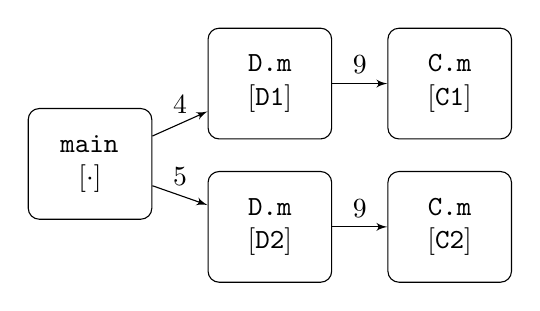
\begin{tikzpicture}
		\node [block] (main) {{\tt main$_{}$}\\$[\cdot]$};
		\node [block, above right = -0.4cm and
		0.7cm of main] (Dm1) {\tt {D.m}\\$[$D1$]$};
		\node [block, below = 0.4cm of Dm1] (Dm2) {\tt{D.m}\\$[$D2$]$};
		\node [block, right = 0.7cm of Dm1] (Cm1) {\tt{C.m}\\$[$C1$]$};
		\node [block, right = 0.7cm of Dm2] (Cm2) {\tt{C.m}\\$[$C2$]$};
		
		\path [line] (main) edge node[above] {$4$} (Dm1);
		\path [line] (main) edge node[above] {$5$} (Dm2);
		\path [line] (Dm1) edge node[above] {$9$} (Cm1);
		\path [line] (Dm2) edge node[above] {$9$} (Cm2);
		\end{tikzpicture}
    }
    \end{center}
}
where $I_1 = \emptyset$ and $I_2 = \myset{9}$. 
% A detail example is described in Section 1.2 of our supplementary material~\footnote{\url{https://zenodo.org/record/5560499}}.
      %Appendix~\ref{sec:unwrapped}.
% Without context tunneling, $1$-call-site-sensitivity merges
% two {\tt C.m} method calls under context of \texttt{[9]}.
% By applying context-tunneling to invocations in $I_2$, however, 
% the method calls inherit contexts from their callers,
%  \texttt{[4]} and \texttt{[5}] respectively, thus becomes 
% as precise as $1$-object-sensitivity.

%\textcolor{red}{
%Intuitively, the invocation-sites in a tunneling abstraction ($\Tcall$) are considered as bad context elements for call-site sensitivity; the invocation-sites will not be used as context elements. The tunneling abstraction $I_1\cup I_2 = \myset{5,7,8}$ considers the invocation-sites 5,7,8 as bad elements because they make call-site sensitivity produce a different context abstraction from the given object sensitivity.
%}


Note that applying context tunneling at $I_1\cup I_2 = \myset{5,7,8}$
makes call-site sensitivity simulate the baseline object
sensitivity (Figure~\ref{fig:call:callgraph} and Figure~\ref{fig:obj:callgraph} are equivalent). However, it loses the precision benefit of the original call-site
sensitivity (compare Figure~\ref{fig:call:callgraph}
vs. Figure~\ref{fig:CFA:callgraph}).
The purpose of $I_3$ is to avoid this precision loss. 
We define $I_3$ to be the set of invocation-sites where the called
  method has a single context:
\[
I_3 = \myset{l \in \Invo_P \mid \forall (l, c_1, m, c_1'), (l, c_2,
	m, c_2') \in G.\; c_1' = c_2'}.
\]
% where the edges $(l, c_1, m_1, c_1')$ and $(l, c_2,
%   m_2, c_2')$ can be identical.
In Figure~\ref{fig:obj:callgraph}, $I_3$ equals to $\myset{7, 8, 16,
  17, 18}$. For example, $I_3$ includes 7 because only one call-graph
edge exists out of that invocation-site and $I_3$ does not include 5
because it has two outgoing edges to the same method ({\tt id}) under
different contexts ({\tt [D1]} and {\tt [D2]}).
%$I_3$ guarantees that call-site sensitivity analyzes the called method
%more precisely than (or at least equal to) object sensitivity.\minseok{Check} This is because
Intuitively, 
$I_3$ represents the set of invocation-sites that make conventional call-site sensitivity %, which always updates contexts, 
 at least as precise as the given object sensitivity; avoiding context tunneling at 
$I_3$ would make call-site sensitivity analyze the called method
more precisely than (or at least equal to) object sensitivity.
 It is because updating context with the invocation sites ensures that the method invocation is not conflated with another invocation from different invocation-sites which is not the case for object sensitivity.
%It is because conventional call-site sensitivity separates methods called from an invocation-site from the others which is not the case for object sensitivity.
%Updating contexts at $I_3$ ensures that the method invocation is not conflated with another invocation from different invocation-sites.
%As object sensitivity failed to separate any of the methods invoked in $I_3$.
%The intuition behind $I_3$ is leveraging a property of conventional call-site sensitivity that methods called from an invocation-site is guaranteed to be separated from the ones called from the other invocation-sites which is not the case for object sensitivity. 
%Updating contexts at $I_3$ would ensures that the method invocation is not conflated with another invocation from different invocation-sites, which is not the case for
%object sensitivity.
%This is because
%it ensures that the method invocation is not conflated with another
%invocation from different invocation-sites, which is not the case for
%object sensitivity. 
%Figure~\ref{fig:opt:callgraph} shows the resulting call-graph
In summary, we infer $\Tcall = \myset{5}$ from
Figure~\ref{fig:obj:callgraph}: 
 $\Tcall = (I_1 \cup I_2)  \setminus I_3 = (\myset{5,7,8} \cup \myset{5})
 \setminus \myset{7,8,16,17,18}
= \myset{5}$. 

%\textcolor{red}{
Additionally, we apply context tunneling to the invocation-sites if all their parameters are passed from those of the caller methods. 
For example, $\myset{5}$ in our example
belongs to this case because all the parameters (i.e., \texttt{this} and \texttt{v}) come from the caller. 
Such invocations need context tunneling because caller methods' contexts determine the value of the parameters.
For the same reason, we avoid context tunneling if all the parameters
are allocated just before the invocations (e.g., $\myset{16, 17}$ in
our example). The invocation-sites are useful because using them as context elements determines the value of the invocations' parameters.

% !TEX root = ./paper.tex

\input{Obj2CFA/wrappedflow}

\myparagraph{Effectiveness in the Real-World}\label{sec:simulation:real-world}
To show the effectiveness of simulation more clearly, we provide a representative real-world example.
%In this example, we aim to show that call-site sensitivity with tunneling can effectively analyze the representative example, and call-site sensitivity 
Also, this example shows that call-site sensitivity can simulate object sensitivity with a nontrivial tunneling abstraction ($\Tobj \neq \emptyset$).



%\textcolor{red}
{
Containers and iterators have been popular to exemplify the strength
of object sensitivity (e.g.~\cite{Milanova2005,JeJeOh18,TanLX16}), as
they are prevalent in object-oriented
programs.
Figure~\ref{fig:wrappedflow:example} shows a typical example.
%, called {\em wrapped flow}~\cite{Li2018a}.
In Figure~\ref{fig:wrappedflow:example}, the {\tt Container} class has
its iterator of which the field wraps the container's
data, and the data is obtained by the calling iterator's method.
}

%\textcolor{red}
{
In this case, 1-object sensitivity needs context tunneling to distinguish all the method calls.
The conventional 1-object-sensitive analysis is not precise as
the two iterators share the same heap allocation-site {\tt It}. 
Consider a tunneling abstraction
$\Tobj =\{7, 21, 26\}$.
With this tunneling abstraction, 1-object sensitivity produces precise
results with the
call-graph shown in Figure~\ref{fig:wrappedflow:1objTGraph}.
}


\begin{figure*}
\begin{center}
%\begin{subfigure}[b]{1\columnwidth}
%\begin{multicols}{2}

%\end{multicols}
%\end{subfigure}
\begin{multicols}{2}
	\begin{subfigure}[b]{\columnwidth}
	\centering
		\begin{center}
			\resizebox{.9\columnwidth}{!}{
				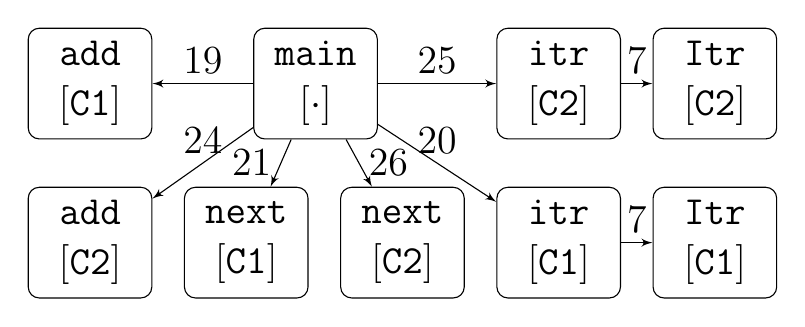
\begin{tikzpicture}
                \tikzstyle{every node}=[font=\Large]
				\node [block] (main) {\tt {main}\\$[\cdot]$};
				
				\node [block, left = 1.28cm of main] (add1) {\tt {add}\\$[$C1$]$};
				\node [block, below = 0.6cm of add1] (add2) {\tt {add}\\$[$C2$]$};
				
				\node [block, right = 0.4cm of add2] (next1) {\tt {next}\\$[$C1$]$};
				\node [block, right = 0.4cm of next1] (next2) {\tt {next}\\$[$C2$]$};
				
				\node [block, right=0.4cm of next2] (itr1) {\tt {itr}\\$[$C1$]$};
				\node [block, above=0.6cm of itr1] (itr2) {\tt {itr}\\$[$C2$]$};
				
				\node [block, right=0.4cm of itr1] (Itr1) {\tt {Itr}\\$[$C1$]$};
				\node [block, right=0.4cm of itr2] (Itr2) {\tt {Itr}\\$[$C2$]$};
				
				
				\path [line] (main) edge node[above] {$19$} (add1);
				\path [line] (main) edge node[above] {$24$} (add2);
				
				\path [line] (main) edge node[left] {$21$} (next1);
				\path [line] (main) edge node[right] {$26$} (next2);
				
				\path [line] (main) edge node[above] {$20$} (itr1);
				\path [line] (main) edge node[above] {$25$} (itr2);
				
				\path [line] (itr1) edge node[above] {$7$} (Itr1);
				\path [line] (itr2) edge node[above] {$7$} (Itr2);
				
				
				\end{tikzpicture}
			}
		\end{center}
		\caption{$1$-object sensitivity with $T_{\it obj}=\myset{7,21,26}$}
		\label{fig:wrappedflow:1objTGraph}
	\end{subfigure}
	\vfill\null
	\columnbreak
	\begin{subfigure}[b]{\columnwidth}
		\begin{center}
			\resizebox{.9\columnwidth}{!}{
				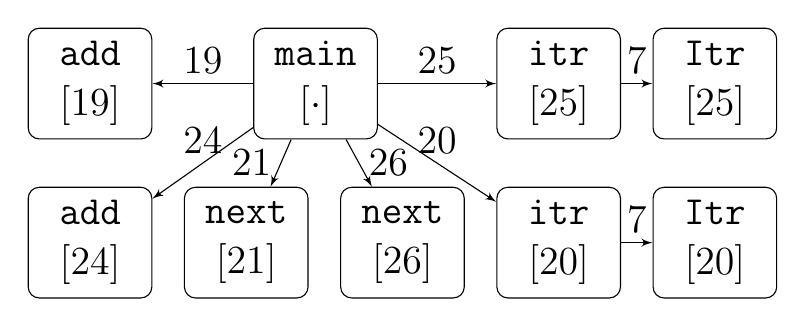
\begin{tikzpicture}
                \tikzstyle{every node}=[font=\Large]
				\node [block] (main) {\tt {main}\\$[\cdot]$};
				
				\node [block, left = 1.28cm of main] (add1) {\tt {add}\\$[19]$};
				\node [block, below = 0.6cm of add1] (add2) {\tt {add}\\$[24]$};
				
				\node [block, right = 0.4cm of add2] (next1) {\tt {next}\\$[21]$};
				\node [block, right = 0.4cm of next1] (next2) {\tt {next}\\$[26]$};
				
				\node [block, right=0.4cm of next2] (itr1) {\tt {itr}\\$[20]$};
				\node [block, above=0.6cm of itr1] (itr2) {\tt {itr}\\$[25]$};
				
				\node [block, right=0.4cm of itr1] (Itr1) {\tt {Itr}\\$[20]$};
				\node [block, right=0.4cm of itr2] (Itr2) {\tt {Itr}\\$[25]$};
				
				
				\path [line] (main) edge node[above] {$19$} (add1);
				\path [line] (main) edge node[above] {$24$} (add2);
				
				\path [line] (main) edge node[left] {$21$} (next1);
				\path [line] (main) edge node[right] {$26$} (next2);
				
				\path [line] (main) edge node[above] {$20$} (itr1);
				\path [line] (main) edge node[above] {$25$} (itr2);
				
				\path [line] (itr1) edge node[above] {$7$} (Itr1);
				\path [line] (itr2) edge node[above] {$7$} (Itr2);
				
				
				\end{tikzpicture}
			}
			
		\end{center}
		\caption{$1$-call-site sensitivity with $T_{\it call}=\myset{7}$}
		\label{fig:wrappedflow:1callTGraph}
	\end{subfigure}
\end{multicols}
\vspace{-30pt}
\caption{call-graphs produced by
1-object sensitivity with context-tunneling and 1-call-site
sensitivity}
\vspace{-12pt}
\label{fig:wrappedflow}
\end{center}
\end{figure*}

%\textcolor{red}
{
With our technique, call-site-sensitivity can simulate the call-graph
produced by the context-tunneled object-sensitive analysis. 
From the call-graph in Figure~\ref{fig:wrappedflow:1objTGraph}, our
technique finds out
\[
I_1 = \myset{7}, \quad  I_2 = \{7\},\quad I_3 =
\{19,20,21,24,25,26\}.
\]
and produces a tunneling abstraction $\Tcall = \{7\}$.
Figure~\ref{fig:wrappedflow:1callTGraph} shows the call-graph of
1-call-site sensitivity with the tunneling abstraction, which is
exactly the same as that of the baseline object-sensitive analysis
in Figure~\ref{fig:wrappedflow:1objTGraph}.
Note that 1-object sensitivity and 1-call-site sensitivity use
different tunneling abstractions, i.e., $\Tcall = \{7\}$ vs.
$\Tobj = \{7, 21, 26\}$. 
}





%\textcolor{red}{
%\myparagraph{Effectiveness in the Real-World}
%The simulation technique described above is principled (i.e., it exploits fundamental properties of context-tunneled call-site sensitivity) and yet powerful
%enough to make call-site sensitivity to enjoy most of the precision
%benefits of object sensitivity in practice. For example, our technique
%enables 1-call-site sensitivity to effectively handle all
%patterns of {\em precision-critical} methods
%in~\cite{Li2018a}.  
%\citet{Li2018a} identified fairly representative and
%exhaustive patterns that require object sensitivity in real-world Java
%programs;
%applying 2-object sensitivity only to the methods with those patterns
%is sufficient to achieve 98.8\% of the full precision~\cite{Li2018a}. 
%Conventional call-site-sensitive analysis is
%ineffective to handle such patterns as they require the
%analysis to maintain deep calling contexts. With context tunneling,
%however, our technique enables call-site
%sensitivity to simulate object sensitivity in all cases. We provide
%detailed description of the patterns and how our technique works in
%Appendix~\ref{appendix:effectiveness}. 



\myparagraph{Simulated Policy}
Now we define the simulated policy $\simheuristic$. 
Let $\simulate$ be the simulation process described above. 
As input, $\simulate$ takes a program $P$ and a tunneling abstraction
$\Tobj \subseteq \Invo_P$ of baseline object sensitivity.  
Running the simulation procedure, denoted $\simulate(P, \Tobj)$, produces a tunneling abstraction $\Tcall \subseteq
\Invo_P$ for call-site sensitivity.  
With $\simulate$, we can transform $\objheuristic$ into
$\simheuristic$ as follows:
\begin{equation}\label{eq:simheuristic}
  \simheuristic = \lambda P.\; \simulate(P,
  \objheuristic(P)).
\end{equation}
Although the simulated policy $\simheuristic$ makes call-site
sensitivity more precise than the baseline object sensitivity, using
$\simheuristic$  is
impractical because the simulation procedure incurs the overhead of running the baseline object-sensitive analysis.






%%% Local Variables:
%%% mode: latex
%%% TeX-master: "paper"
%%% End:

\clearpage
\subsection{Learning Algorithm}
Now we illustrate our learning algorithm that learns heuristic
$\heuristic_\params$ from codebases $\vec{P}$.
The goal of our algorithm is to find $\params$ where
%$\heuristic_\params$ would produce minimal abstractions for the training programs.
$\heuristic_\params$ produces minimal abstractions for the training programs.
Let $A_P$ be a minimal abstraction of a program $P$.
The learning objective is as follows:
\[
\mbox{Find $\params = \myvec{\Feat_1, \Feat_2,\dots,\Feat_k}$
  that }\forall P\in\vec{P}. \heuristic_\params({\projgraph}
(F_P(\lambda c \in \component_P.0))) \approx A_P(P)
\]
%The insight behind the learning objective is that we expect learned
%heuristic would produce a suitable abstraction
The insight behind this objective is that the learned
heuristic would produce a minimal abstraction
for other programs as it was trained to produce minimal abstractions
for the training programs.


\begin{algorithm}[t]
	\caption{Overall learning algorithm}\label{alg:overall}%\small
	\begin{algorithmic}[1]
		\Require Training programs $\vec{P}$, static analyzer $F$, maximum abstraction degree $k$
		\Ensure Parameters $\myvec{\Feat_1,\Feat_2,\dots,\Feat_k}$
		\Procedure{Learn}{$\vec{P}, F, k$}
		\State
		$\myvec{\Feat_1,\Feat_2,\dots,\Feat_k} \gets \myvec{\emptyset,\emptyset,\dots,\emptyset}$
		\State
		$A_\vec{P} \gets \lambda P \in \vec{P}. {\LearnMinimalAbstraction}(P,F,k)$ \Comment{mapping programs to minimal abstractions}
		\State
		$G_\vec{P} \gets \lambda P\in \vec{P}.{\projgraph}(F_P(\absz))$ \Comment{mapping programs to graphs from pre-analysis}
		\For{$i=1$ to $k$}
                \State
			$\Feat_i \gets \LearnSetOfFeatures(i,A_\vec{P},G_\vec{P})$
		\EndFor
		\State \Return $\myvec{\Feat_1,\Feat_2,\dots,\Feat_k}$
		\EndProcedure
	\end{algorithmic}
\end{algorithm}




\myparagraph{Overall Algorithm}
Algorithm~\ref{alg:overall} presents the overall algorithm. The
parameter $\params$ starts with a vector of empty sets
$\myvec{\emptyset,\emptyset,\dots,\emptyset}$.
First, the algorithm obtains minimal abstractions $A_\vec{P}$ and
graph $G_\vec{P}$  over the training
programs $\vec{P}$ at line 3 and 4. $A_\vec{P}$ presents minimal
abstractions over the training programs where $A_\vec{P}$ maps each
%programs' component to a minimal abstraction degree while preserving
component of programs to a minimal abstraction degree while preserving
the full precision.
With the minimal abstractions $A_\vec{P}$ and a graph $G_\vec{P}$, the algorithm
%learns each set of features $G_i$ that presents nodes that need abstraction degree $i$.
learns each set of features $G_i$ presenting the nodes which requires abstraction degree $i$.
The function $\textsc{LearnSetofFeatures}$ takes minimal abstractions
$A_\vec{P}$, a graph $G_\vec{p}$, and an abstraction degree $i$ as
inputs.
%It returns a set of features $\Feat_i$ that presents nodes that need to be assigned $i$.
It returns a set of features $\Feat_i$ which depicts the nodes to be assigned $i$.
%Although we write $G_i$ is obtain iteratively, we can parallely learn $G_i$ to reduce learning costs.
Although $G_i$ is obtained iteratively in the algorithm, we can learn it in parallel to reduce the learning cost.
The algorithm ends if it gets all the sets of features $\Feat_1,
\Feat_2,\dots, \Feat_k$, and returns $\myvec{\Feat_1, \Feat_2,\dots, \Feat_k}$ as a parameter $\params$.


\clearpage

\begin{algorithm}[t]
	\caption{Learning minimal abstraction}\label{alg:Learnminimal}%\small
	\begin{algorithmic}[1]
			\Require Program $P$, static analyzer $F$, maximum abstraction degree $k$
		\Ensure A minimal abstraction for $P$
		\Procedure{\LearnMinimalAbstraction}{$P,F,k$} 
		\State
		$C \gets \component_{P}$
		\State
		$\abs \gets \lambda c. k$
		\For{$i=k$ to 1}
		\State
		$C' \gets C$
		\While {$C' \neq \emptyset$}
			\State
			$c' \gets pick(C')$
			\State
			$C' \gets C' \setminus \{c'\}$
			\State
			$\abs' \gets \lambda c. {\it if}~c=c'~{\it then}~i-1~{\it else}~\abs(c)$
			\If {${\projproved}(F_P(\absk)) = {\projproved}(F_P(\abs'))$}
				\State
				$\abs \gets \abs'$
			\EndIf
		\EndWhile
		\State
		$C \gets C \setminus \{c \mid \abs(c) = i\}$
		\EndFor
		\State \Return $\abs$
		\EndProcedure
	\end{algorithmic}
\end{algorithm}



\myparagraph{Getting Minimal Abstractions}
Algorithm~\ref{alg:Learnminimal} presents our efficient algorithm to
obtain a minimal abstraction for a given program $P$.
Searching minimal abstractions for a program $P$ poses a huge search space $k^{\component_P}$.
%$(k+1)^C$ where $C$ presents all program components in the codebases.
%Our algorithm reduces the search space into $k*C$ while guarantees to find minimal abstractions.
Our algorithm reduces the search space into $k*C$ but still guarantees to find minimal abstractions.
At line 2, $C$ gets all the program components in $P$.
$\abs$ starts from the most precise one; it always assigns $k$.
At line 4 -- 15, it iteratively refines $\abs$ toward a minimal abstraction.
In each iteration, it finds program components that needs abstraction degree $i$ in the minimal abstraction
where $i$ is equal to $k$ at a start point and decreases as the loop iterates.
At line 5, it collects free program components $C'$ which are not determined their 
abstraction degree in the minimal abstraction; it equals to $\component_P$ in the first iteration.
At line 6 -- 13, it iteratively picks a component $c'$ in $C'$ and decreases its abstraction 
degree by 1~(e.g., assign $i-1$) in \abs. If the refined abstraction $\abs'$ is still precise 
(e.g., ${\projproved}(F_P(\absk)) = {\projproved}(F_P(\abs'))$), it accepts the refinement.
If it violates the precision constraint, the algorithm rejects the refinement, and the abstraction degree of the program component $c'$ is determined as $i$. 
At line 14, it subtracts the determined components from $C$.
The algorithm ends after it learns program components that need $1$;
$\abs$ assigns $0$ to the remaining ones in $C$.
In worst case, our algorithm searches
$k*\component_P$ different abstractions as search space of each iteration is
at most $\component_P$, and the algorithm has $k$ iterations.
Although the algorithm considers much less search spaces than the original one
$(k+1)^C$, it still guarantees to find minimal abstractions:
\begin{theorem}\label{THM:REDUCESPACE}
The abstraction $A_\vec{P}$ returned from
Algorithm~\ref{alg:Learnminimal} corresponds to minimal abstractions over the
codebases $\vec{P}$.
\end{theorem}
\begin{proof}
See Appendix~\ref{sec:proof}.
\end{proof}
%Our algorithm is a generalized one from~\citet{Liang2011learning}.
Our algorithm is an advanced version of~\citet{Liang2011learning}.
The prior algorithm searches all the abstraction space (e.g., $C^{k}$) without reduction.
Our one, however, reduces the search space into a small one(e.g., $C*{k}$) but
still guarantees to find minimal abstractions.

\clearpage
\begin{algorithm}[t]
	\caption{Learning a set of features}\label{alg:learnFeatures}\small
	\begin{algorithmic}[1]
		\Require Abstraction level $i$, minimal abstractions $A_\vec{P}$, graphs $G_\vec{P}$
		\Ensure A set of abstract features $\Feat$
		\Procedure{LearnSetOfFeatures}{$i,A_\vec{P},G_\vec{P}$}
		\State
		$C \gets \{c \mid P \in \vec{P}\land c \in \component_P \land A_\vec{P}(P)(c) = i\}$
		\State
		$\Feat \gets \emptyset$
                \While {$C \not = \emptyset $}
                \State $\feature \gets {\textsc LearnFeature}(C,G_\vec{P})$ \Comment Learn abstract graph
                \State $\Feat \gets \Feat \cup \feature$
                \State $C \gets C \setminus \{c \mid P\in\vec{P}\land c\in \component_P \land c \in \sem{\feature}_{G_\vec{P}(P)} \}$
                \EndWhile
                \State \Return $\Feat$
		\EndProcedure
	\end{algorithmic}
\end{algorithm}


\myparagraph{Learning a Set of Features}
%Algorithm~\ref{alg:learnFeatures} presents how to learn a set of features $\Feat_i$.
Algorithm~\ref{alg:learnFeatures} describes a learning algorithm for a set of features $\Feat_i$.
%The algorithm takes an abstraction level $i$, minimal abstractions $A_\vec{P}$, and graphs $G_\vec{P}$ as inputs.
It takes an abstraction level $i$, minimal abstractions $A_\vec{P}$, and graphs $G_\vec{P}$ as inputs.
It returns as an output a set of features $\Feat$ presenting nodes that require an abstraction degree $i$ (e.g., $\Feat_i$ in Algorithm~\ref{alg:overall}).
%The goal of this algorithm is to convert the program components to be assigned $i$ into a set of features $\Feat$.
The goal of this algorithm is to convert the program components to which $i$ will be assigned to a set of features $\Feat$.
%The returned features cover all the program components:
Thereby, the returned features can cover the components assigned $i$:
\[ \forall P\in\vec{P}. \{c \mid c \in \component_P \land A_\vec{P}(P)(c) = i\}
\setminus \{ c \mid c\in \component_P \land \sem{\Feat}_{G_\vec{P}(P)} \}  = \emptyset.
\]
At line 2, it collects all program components $C$ (e.g., nodes) to which the minimal abstraction
assigns $i$.
At line 3, it initializes $\Feat$  as an empty set.
At line 4--8, the algorithm iteratively calls ${\textsc LearnFeature}$ to generate a feature.
The algorithm adds the generated features to $\Feat$ until the
features cover all program components, and returns $\Feat$ as learned features when $\Feat$ does.
%If $\Feat$ does, the algorithm returns $\Feat$ as learned features.

%In each iteration, the algorithm generates a feature $\feature$.
%${\textsc LearnGHat}$ takes the components $C_i$ and graphs
%$G_\vec{P}$ and generate a feature $\feature$ that
%${\textsc LearnGHat}$ tries to make the feature maximize the following function:

\algdef{SE}[DOWHILE]{Do}{doWhile}{\algorithmicdo}[1]{\algorithmicwhile\ #1}%
%Ver. 2
\begin{algorithm}[t]
	\caption{Learning a feature}\label{alg:learnFeature}\small
	\begin{algorithmic}[1]
		\Require Program components $C$, graphs $G_\vec{P}$
		\Ensure A feature $\feature$
		\Procedure{LearnFeature}{$C,G_\vec{P}$}
		\State
		$\feature \gets
				(\epsilon,([0,\infty],[0,\infty]),\epsilon)$
		\State
		$\feature' \gets
				(\epsilon,([0,\infty],[0,\infty]),\epsilon)$
		\Do
		\State
		$\feature \gets \feature'$
		\State
		$\feature' \gets \Refine(\feature,G_\vec{P}, C)$
		\If{$\Score(\feature',C_i) \ge \gamma$}
			\State
			\Return $\feature'$
		\EndIf
		\doWhile{$ \Score(\feature',C) > \Score(\feature,C)$}
		
%		\While {$ (\Score(\feature',C) > \Score(\feature,C)$)}
%		\State
%		$\feature \gets \feature'$
%		\If {$\Score(\feature',C) \ge \gamma$}
%		\State
%			\Return $\feature'$
%		\EndIf
%		\State
%		$\feature' \gets \Refine(\feature,G_\vec{P}, C)$
%                % \If {$( \Score(\feature',C_i) \ge \gamma$}
%                % \State
%                % \Return $\feature'$
%                %\EndIf
%		\EndWhile
		\State \Return $\feature$
		\EndProcedure
	\end{algorithmic}
\end{algorithm}



\myparagraph{Learning a Feature}
%Algorithm~\ref{alg:learnFeature} presents the algorithm that generates each feature.
%Algorithm~\ref{alg:learnFeature} presents how a feature $\feature$ is learned.
Algorithm~\ref{alg:learnFeature} presents how each feature $\feature$ in $\Feat$ is learned.
%${\textsc LearnFeature}$ takes oracle components $C$ and graphs $G_\vec{P}$. 
%It tries to generates a feature $\feature$ that maximizes the following function:
${\textsc LearnFeature}$ takes as inputs oracle components $C$ and graphs $G_\vec{P}$,
and generates a feature $\feature$ 
which has a good enough score presented by the following function:
%maximizes the following score function of a feature $\feature$:
\[
\Score (\feature,G_\vec{P},C) = {\sum_{P\in\vec{P}} |C \cap \sem{\feature}_{G_\vec{P} (P)}  | \over
  \sum_{P\in\vec{P}} |\sem{\feature}_{G_\vec{P}(P)} |}
\]
where the score is a value between 0 and 1.
%Intuitively, it is a score function of a feature $\feature$.
%If a feature $\feature$ accurately selects component in oracle that $\sum_{P\in\vec{P}}\sem{\feature}_{G_\vec{P} (P)}$ belongs to $C$,
%the score become the highest one 1.
For example, the score is the highest value 1 
if a feature $\feature$ accurately selects a component in oracle 
where $\sum_{P\in\vec{P}}\sem{\feature}_{G_\vec{P} (P)}$ belongs to $C$.
Collecting qualified feature make the learned parameter
$\params = \myvec{\Feat_1, \Feat_2,\dots,\Feat_k}$ satisfy the learning objective.
%The score decreases when the feature selects components which are not in $C$.
The score decreases when the feature selects components not in $C$.

Starting from the most general feature, 
the algorithm iteratively refines a feature until the specific feature is generated.
%At line 2, it initializes a feature as the most general one.
%$\MaxIn(G_\vec{P})$ and $\MaxOut(G_\vec{P})$ present the
%maximum number of incoming and outgoing edges of a node in the
%graphs, respectively (see Appendix~\ref{sec:max}).
At line 2, it initializes a feature $\feature$ as the most general feature $(\epsilon,([0,\infty],[0,\infty]),\epsilon)$.
%as all nodes in any graphs belong to this feature.
%$(\epsilon,([0,\infty],[0,\infty]),\epsilon)$ is the most general feature as all the nodes in any graph belong to it.
At line 4--10, the algorithm iteratively calls $\Refine$ to specify the feature $\feature$ 
into various cases and to select the best one among them:
%$\Refine$ specifies a given feature $\feature$ into various cases and selects the best one:
\[\Refine(\feature,G_\vec{P},C_i) =
argmax_{\feature' \in New(\feature,G_\vec{P}) \cup Replace(\feature)}(\Score(\feature',G_\vec{P},C_i))
\]
where $\New(\feature,G_\vec{P})$ and $\Replace(\feature)$ produce features
%specified from $\feature = (lst,i)$ by appending or replacing a node of the $lst$.
specified from $\feature$ by appending or replacing an abstract node in the feature:
%$\New(\feature,G_\vec{P})$ produces features which are specified by appending an abstract node:
$\New(\feature,G_\vec{P})$ produces the specificed features by appending an abstract node:
\[
\begin{array}{lr}
\New((\seq{\hat{p}_0,\hat{p}_1,\dots,\hat{p}_q}, \hat{n}, \seq{\hat{s}_0,\hat{s}_1,\dots,\hat{s}_r}),G_\vec{P}) =\\
\{((\seq{\hat{n}',\hat{p}_0,\hat{p}_1,\dots,\hat{p}_q}, \hat{n}, \seq{\hat{s}_0,\hat{s}_1,\dots,\hat{s}_r})) \cup (\seq{\hat{p}_0,\hat{p}_1,\dots,\hat{p}_q}, \hat{n}, \seq{\hat{s}_0,\hat{s}_1,\dots,\hat{s}_r,\hat{n'}}) \mid\\ n' \in
  \Specify(([0,\infty],[0, \infty])) \}. 
%  \Specify(([0,\MaxIn(G_\vec{P})],[0, \MaxOut(G_\vec{P})])) \}
\end{array}
\]
We do not consider $\New(\feature,G_\vec{P})$ if the length of $\feature$ is 3 (e.g., $len(\seq{\hat{p}_0,\hat{p}_1,\dots,\hat{p}_q})+1+len(\seq{\hat{s}_0,\hat{s}_1,\dots,\hat{s}_r}) = 3$)
because we found a feature $\feature$ which is longer than 3 yields bottleneck when computing $\sem{\feature}_{G_\vec{P}(P)}$.
The function $\Specify$ takes as an input an abstract node and returns 4 cases of specified nodes:
\[
\begin{array}{l}
\Specify(([n_1,n_2],[n_3,n_4])) = \\
\{([{{n_1+n_2}\over {2}},n_2],[n_3,n_4]),
([n_1,{{n_1+n_2} \over {2}} ],[n_3,n_4]),
([n_1,n_2], [{{n_3+n_4}\over {2}}, n_4]),
([n_1,n_2],[n_3,{{n_3+n_4}\over{2}} ])\}.
    \end{array}
\]
Above enumeration is one of a choice in specifying an abstract node. 
For example, we can use a more fine grained enumeration that specifies a feature into 8 cases by splits 
an interval $[a,b]$ into 4 cases:
$\{[{{a+b}\over {3}},b],[{2*{(a+b)}\over {3}},b], [a,{{a+b}\over {3}}], [a,{{2*(a+b)}\over {3}}]\}$.
Employing a fine grained one, however, would increase the learning time because the algorithm searches
about double cases of features.
If $n_2$ or $n_4$ equals to $\infty$, they are replaced to either $\MaxIn(G_\vec{P})$ or $\MaxOut(G_\vec{P})$; 
$\MaxIn(G_\vec{P})$ and $\MaxOut(G_\vec{P})$ represent the maximum number of incoming and outgoing edges of a node in the graphs $G_\vec{P}$ ,respectively (see Appendix~\ref{sec:max}).
On the other hand, $\Replace(\feature)$ refines the given feature $\feature$ by specifying an abstract node inside the feature:
\[
\begin{array}{c}
\Replace((\seq{\hat{p}_0,\hat{p}_1,\dots,\hat{p}_q}, \hat{n}, \seq{\hat{s}_0,\hat{s}_1,\dots,\hat{s}_r})) =
  \{(\hat{\vec{p}}',\hat{n},\hat{\vec{s}}) \cup (\hat{\vec{p}},\hat{n}',\hat{\vec{s}}) \cup (\hat{\vec{p}},\hat{n},\hat{\vec{s}}') \mid \\
\hat{\vec{p}}' =
\seq{\hat{p}_0,\hat{p}_1,\dots,\hat{p}_{i-1},\hat{p}_i',\hat{p}_{i+1},\dots\hat{p}_q} \land \hat{p}_i' \in \Specify(\hat{p}_i)
\land n' \in \Specify(n_i) \land\\
\hat{\vec{s}}' =
\seq{\hat{s}_0,\hat{s}_1,\dots,\hat{s}_{j-1},\hat{s}_j',\hat{s}_{j+1},\dots,\hat{s}_r} \land \hat{s}_j' \in \Specify(\hat{s}_j)
\end{array}
\]
where $\hat{\vec{p}}=\seq{\hat{p}_0,\hat{p}_1,\dots,\hat{p}_q}$ and $\hat{\vec{s}}=\seq{\hat{s}_0,\hat{s}_1,\dots,\hat{s}_r}$.
The algorithm refines the feature $\feature$ until the function
$\Refine$ fails to find a better feature or the refined feature has a better score than $\gamma$
which is a hyper parameter to control the generalization of generated feature.
If $\gamma$ is 1, the generated feature would overfit to the training programs;
thereby, setting $\gamma$ as a lower value makes the generated feature to avoid overfitting problem.
In our evaluation, we set $\gamma$ as 0.5. 
%Further, we limit the maximum overall length of a feature as 3 (e.g., $len(\seq{\hat{p}_0,\hat{p}_1,\dots,\hat{p}_q})+1+len(\seq{\hat{s}_0,\hat{s}_1,\dots,\hat{s}_r}) \le 3$)
%because we found a feature $\feature$ which is longer than 3 yield bottleneck when computing $\sem{\feature}_{G_\vec{P}(P)}$.


\begin{comment}
\[
\begin{array}{lr}
\New((\seq{\hat{p}_0,\hat{p}_1,\dots,\hat{p}_q}, \hat{n}, \seq{\hat{s}_0,\hat{s}_1,\dots,\hat{s}_r}),G_\vec{P}) =\\
\{((\seq{\hat{n}',\hat{p}_0,\hat{p}_1,\dots,\hat{p}_q}, \hat{n}, \seq{\hat{s}_0,\hat{s}_1,\dots,\hat{s}_r})) \cup (\seq{\hat{p}_0,\hat{p}_1,\dots,\hat{p}_q}, \hat{n}, \seq{\hat{s}_0,\hat{s}_1,\dots,\hat{s}_r,\hat{n'}}) \mid\\ n' \in
  \Specify(([0,\infty],[0, \infty])) \}.
%  \Specify(([0,\MaxIn(G_\vec{P})],[0, \MaxOut(G_\vec{P})])) \}
\end{array}
\]
The function $\Specify$ takes an abstract node and returns 4 cases of specified nodes:
\[
\begin{array}{l}
\Specify(([n_1,n_2],[n_3,n_4])) = \\\{([{{n_1+n_2}\over {2}},n_2],[n_3,n_4]),
([n_1,{{n_1+n_2} \over {2}} ],[n_3,n_4]),
([n_1,n_2], [{{n_3+n_4}\over {2}}, n_4]),
([n_1,n_2],[n_3,{{n_3+n_4}\over{2}} ])\}
\end{array}
\]
If $n_2$ or $n_4$ equals to $\infty$, they are replaced to $\MaxIn(G_\vec{P})$ or $\MaxOut(G_\vec{P})$; $\MaxIn(G_\vec{P})$ and $\MaxOut(G_\vec{P})$ present
maximum number of incoming and outgoing edges of a node in the graphs $G_\vec{P}$ ,respectively (see Appendix~\ref{sec:max}).
On the other hand, $\Replace(\feature)$ refines the given feature by
specifying an abstract node in it:
\[
\begin{array}{c}
\Replace((\seq{\hat{p}_0,\hat{p}_1,\dots,\hat{p}_q}, \hat{n}, \seq{\hat{s}_0,\hat{s}_1,\dots,\hat{s}_r})) =
  \{(\hat{\vec{p}}',\hat{n},\hat{\vec{s}}) \cup (\hat{\vec{p}},\hat{n}',\hat{\vec{s}}) \cup (\hat{\vec{p}},\hat{n},\hat{\vec{s}}') \mid \\
\hat{\vec{p}}' =
\seq{\hat{p}_0,\hat{p}_1,\dots,\hat{p}_{i-1},\hat{p}_i',\hat{p}_{i+1},\dots\hat{p}_q} \land \hat{p}_i' \in \Specify(\hat{p}_i)
\land n' \in \Specify(n_i) \land\\
\hat{\vec{s}}' =
\seq{\hat{s}_0,\hat{s}_1,\dots,\hat{s}_{j-1},\hat{s}_j',\hat{s}_{j+1},\dots,\hat{s}_r} \land \hat{s}_j' \in \Specify(\hat{s}_j)
\end{array}
\]
where $\hat{\vec{p}}=\seq{\hat{p}_0,\hat{p}_1,\dots,\hat{p}_q}$ and $\hat{\vec{s}}=\seq{\hat{s}_0,\hat{s}_1,\dots,\hat{s}_r}$.
The algorithm refines the feature $\feature$ until the function
$\Refine$ fails to finds a better feature or the refined feature has a better score than $\gamma$
which is a hyper parameter to control
generalization of generated feature.
If $\gamma$ is 1, the generated feature would overfit to the training programs.
Setting $\gamma$ as a lower value makes the generated feature to avoid overfitting problem.
In our evaluation, we set $\gamma$ as 0.5. Further, we limit the maximum length of a feature as 3.
\end{comment}

\clearpage


% \[
% Fixed(\feature, \feature', C_i)
% = {\sum_{P\in\vec{P}} |C_i \cap \sem{\feature}_{G_P \in \mbg_\vec{P}}  | \over  \sum_{P\in\vec{P}} |\sem{\feature}_{G_P \in \mbg_\vec{P}} | + \epsilon}
% \ge
% {\sum_{P\in\vec{P}} |C_i \cap \sem{\hat{G'}}_{G_P \in \mbg_\vec{P}}  | \over  \sum_{P\in\vec{P}} | \sem{\hat{G'}}_{G_P \in \mbg_\vec{P}} | + \epsilon} * \gamma
% \]






%%% Local Variables:
%%% mode: latex
%%% TeX-master: "paper"
%%% End:

% !TEX root = ./paper.tex



\begin{table}[ht]
	\renewcommand{\arraystretch}{1}
	\caption{Atomic features ($\mba$) used in our method}\label{tbl:obj2cfa:features}
	\centering
	\setstretch{1.1}
	\footnotesize
		 \begin{tabular}{c c c c c c c c c c }
			\toprule
			 A1  & ``java''    & A2  & ``lang''     & A3 & ``sun'' & A4 & ``()'' & A5  & ``void''\\ 
			 A6  & ``security'' & A7 & ``int''      & A8 & ``util'' & A9  & ``String'' &  A10 & ``init''\\ \bottomrule
		 \end{tabular}
		\begin{tabular}{ l l }
			 B1 &  Method is contained in a nested class               \\      
			 B2 & Method contains local assignments                    \\ 
			 B3 & Method contains local variables                      \\ 
			 B4 & Method is contained in a large class                      \\ 
			 B5 & Method contains a heap allocation         \\
			 B6 & Method is a static method         \\
			\midrule
			C1 & Method is called on \texttt{this} (i.e. \texttt{this.$m$(...)}) \\
			C2 & An argument is allocated in the same method      \\ 
			C3 & Method is called on object of static field					\\
			C4 & Method is called else where in the same method \\
			C5 & The base variable is passed to an initializer  \\
			C6 & The containing method's modifier is ``$\texttt{protected}$''        \\
			C7 & The containing method has exception handling        \\
			C8 & All  parameters are passed from caller method\\
			C9 & All  parameters are initialized just before the calls\qquad\,\,\\
			C10 & In ``{\tt java.util.regex}'' class\\
			C11 & Invoke constructor (i.e. \texttt{new C(...)}) \\
			C12 & All the caller method's arguments' type is integer\\
			C13 & Caller method takes more than 2 arguments \\
			C14 & In ``{\tt java.io.*}'' class\\
			C15 & In ``{\tt java.util.logging}'' class \\
			C16 & Takes at least 2 arguments\\
			C17 & Virtual method calls in application class \\
			C18 & Callee method's name is ``{\tt clone}''\\
			C19 & C16 $\land \neg$ C6 $\land \neg$ C1\\
			\bottomrule
		 \end{tabular}
	%\vspace{-10pt}
	\end{table}




\myparagraph{Feature Engineering} 
The success of learning depends also on the atomic features ($\mba$). 
We used a total of 35 atomic features in Table~\ref{tbl:obj2cfa:features},
all of which describe syntactic properties of invocation sites. 
Here, we identify invocations with called methods on them.
Features A1--A10 and B1--B6 came from~\cite{JeJeOh18}. 
% that designed features describing methods in Java programs.}
%Features A1--A10 and B1--B6 came from \citet{JeJeOh18}. 
%Jeon et al.~\cite{JeJeOh18} designed a number of syntactic features of methods. 
Features A1--A10 describe methods whose signatures 
contain the corresponding strings.
For example, when a method's signature string is ``java.lang.String: int length()'', the method has features A1, A2, A4, A7, and A9.
Features B1--B6 describe properties of method bodies. 
For example, feature B1 indicates whether a method is defined in a nested class or not.


Using existing features only was
insufficient 
and we newly designed features C1--C19 in
Table~\ref{tbl:obj2cfa:features}.  In our case, feature engineering was not very difficult as it
can be guided by the simulated policy $\simheuristic$.  To obtain those
features, we initially ran our learning algorithm on training data
with existing features (A1--A10 and B1--B6) only, which resulted in a
parameter $f$ with which the learned policy ($\heuristic_{f}$) did not
satisfy the learning objective. We investigated the reason why $\heuristic_{f}$
fails to capture the behavior of $\simheuristic$ by analyzing the
difference between $\simheuristic$ and $\heuristic_f$ 
(i.e. $\simheuristic(P)\setminus \heuristic_{f}(P)$ and
$\heuristic_{f}(P) \setminus \simheuristic(P)$). 
That is, our goal was to identify features $a_1$ and
$a_2$ that minimize
$\sum_{P\in \vec{P}} \sem{a_1}_P \xor (\simheuristic(P) \setminus
\heuristic_f(P))$ and
$\sum_{P\in \vec{P}} \sem{a_2}_P \xor (\heuristic_f(P) \setminus
\simheuristic(P))$, respectively. 
We included the new 
features $a_1$ and $a_2$ in the feature set and ran the 
algorithm  again. 
We repeated this process until the policy space was large enough to contain solutions and the learning
algorithm could find one of them.
% In our case, the loop iterated 7 times and each iteration produced a
% feature in C1--C7. 
% This feature engineering process was done with training programs only. 
% \minseok{Sunbeom: It seems too expensive, Junhee: feature engineering needs creativity.}








%%% Local Variables:
%%% mode: latex
%%% TeX-master: "paper"
%%% End:

% !TEX root = ./paper.tex

\section{Experimental Results}\label{sec:evaluation}\label{sec:result}
We experimentally prove our claim by evaluating \ourtechnique~on real-world programs. 
Main research questions are as follows: 
%We aim to
%answer the following research questions: 
\begin{itemize}[leftmargin=1.3em]
\item \textbf{Does our claim hold in the real-world?} 
Can call-site sensitivity be significantly superior to object sensitivity for real-world programs? 
How precise and scalable can the
  context-tunneled call-site-sensitive analysis be in practice? 
%  obtained from our
%  technique?
  % effective is out technique that transforms object sensitivity into
  % a context-tunneled call-site sensitivity?
%  How far does it advance the state-of-the-art
%object-sensitive analyses?

%\item \textbf{Effectiveness of simulation and learning:} How
%  accurately can our technique simulate object sensitivity?  Does
%  learning effectively capture the behavior of the simulated policy?
%  Is our learning algorithm essential? How
%  does it compare to simpler approaches?
\item \textbf{Impact of simulation and learning}: 
Is simulation necessary? 
How accurately can our technique simulate object sensitivity?  Is the simulation-guided learning necessary to capture the behavior of the simulated policy? How important are the features in learning?


\end{itemize}


%\input{table_sobj}
%\input{table_2call}

\myparagraph{Experimental Setting}
We implemented \ourtechnique~on top of Doop~\cite{BravenboerS09}, a
popular pointer analysis framework for Java~\cite{JeJeOh18, Li2018b,
  JeJeChOh17, TanLX16, Smaragdakis2014}.  
%\textcolor{red}{Note that superiority of object sensitivity over call-site sensitivity has been consistently demonstrated on Doop~\cite{BravenboerS09,TanLX16,KastrinisS13a,Smaragdakis2014}.}
%To implement our
%popular pointer analysis framework for Java~\cite{JeJeOh18, Li2018b,
%  JeJeChOh17, Tan2017, TanLX16, Smaragdakis2014}.  To implement our
%technique, 
We used the publicly-available implementation of context
tunneling given by \cite{JeJeOh18} and newly implemented our
simulation (Section~\ref{sec:simulation}) and learning
(Section~\ref{sec:learning}) techniques in Doop.  We conducted all
experiments on a machine with Intel i7 CPU and 64GB memory running the
Ubuntu 16.04 64bit operating system.


%\paragraph{Benchmarks}
We used 12 Java programs used by~\cite{JeJeOh18}, of which 10 came from the DaCapo 2006
benchmarks~\cite{Blackburn2006} ({luindex}, {lusearch}, {antlr},
{pmd}, {fop}, {eclipse}, {xalan}, {chart}, {bloat}, and {jython}), and
the remaining two ({checkstyle} and {jpc}) are real-world open-source programs.
%\textcolor{red}{Note that the DaCapo benchmarks also have consistently been used to experimentally demonstrate the superiority of object sensitivity over call-site sensitivity~\cite{Lhotak2006,BravenboerS09,TanLX16}.}
Following prior work~\cite{JeJeOh18,Smaragdakis2014}, we classified those 12
programs into 4 small (luindex, lusearch, antlr, and pmd) and 8 large
programs. 
We used the group of small programs as training data, 
from which our context-tunneling policy $\callheuristic$ is learned, 
and used large programs as test data to evaluate the
policy for unseen programs.


%Pointer analysis START
%analysis time: 123.01s
%Pointer analysis FINISH
%disk footprint (KB)                                                              959,488
%loading statistics (simple) ...
%elapsed time: 11.96s
%
%making database available at /home/minseok/Graphick/Ctx_Sensitivity/doop/results/C-1-tunneled-call-site-sensitive+heap/jre1.6/jython.jar
%making database available at last-analysis
%#var points-to            20,027,400
%#may-fail casts           1,723
%#poly calls               2,498
%#reach methods            12,011
%#call edges               107,112



%\paragraph{Analyses}

Using \ourtechnique, we transformed \oneobjHT, a context-tunneled
1-object-sensitive analysis developed by \cite{JeJeOh18}, into our
1-call-site-sensitive analysis, denoted \ours.  We chose
\oneobjHT~as baseline because it is one of the best object-sensitive analyses
available today, which boosts the conventional 1-object-sensitive
analysis using a well-tuned context-tunneling policy. For
example, \oneobjHT~is empirically more precise than conventional
2-object-sensitive analysis (\twoobjH), which is considered to be highly
precise~\cite{JeJeChOh17,Li2018a,Li2018b,Smaragdakis2014,Graphick20}, yet more
scalable than 1-object sensitivity~\cite{JeJeOh18}.  We obtained the
tunneling policy of {\oneobjHT} from the publicly available artifact
of~\cite{JeJeOh18}.
From {\oneobjHT}, we first applied our simulation
  technique (Section~\ref{sec:simulation}) to produce
  the corresponding simulated call-site sensitivity, denoted \oursim. Then, we
  used our learning algorithm (Section~\ref{sec:learning}) to obtain the final 
   call-site-sensitive analysis, \ours. 
%\[
%\text{\oneobjHT}\xrightarrow[]{\text{simulation}} \text{\oursim} \xrightarrow[]{\text{learning}}\text{\ours}.
%\]
Note that {\oursim} runs {\oneobjHT} as a pre-analysis but {\ours} does not (thanks to learning). 

Our main objective is to compare \oneobjHT~and
\ours, but we compare with some notable analyses as well to
see the advance more clearly. In summary, we compare the following
 analyses:
\begin{itemize}[leftmargin=1.3em]
\item \oneobjHT: a state-of-the-art context-tunneled 1-object-sensitive analysis~\cite{JeJeOh18}
\item \oursim: the simulated 1-call-site-sensitive analysis
    obtained from~\oneobjHT~via 
    simulation% ($\simheuristic$)
\item \ours: our final 1-call-site sensitive analysis
  (obtained from \oursim~via learning)
\item \twoobjH: 2-object-sensitive analysis without
  tunneling~\cite{Smaragdakis2011}
%\item \twocallH: 2-call-site-sensitive analysis without
%  tunneling~\cite{Smaragdakis2011}
\item \onecallHT: the existing state-of-the-art 1-call-site sensitivity with
  tunneling~\cite{JeJeOh18}
\end{itemize}
\twoobjH~is available in Doop. 
\onecallHT~is available in the artifact provided by \cite{JeJeOh18}. 
%\onecallHT~is the existing
%state-of-the-art 1-call-site-sensitive analysis with context
%tunneling, which is available in the artifact of \cite{JeJeOh18}. 
%\textcolor{red}{
%\onecallHT~also boosts the conventional 1-call-site-sensitive analysis. 
%Empirically, \onecallHT~is both more precise and scalable than the conventional 2-call-site-sensitive analysis~\cite{JeJeOh18}.}
All analyses use 1-context-sensitive heap.
For precision metric, we mainly use may-fail
casts. % (\failcasts). % because % it is used in our learning
% algorithm (Section~\ref{sec:learning}) and
%the existing analyses 
%(\oneobjHT~and \onecallHT) have been tuned for it~\cite{JeJeOh18}.
%\begin{comment}
%(\oneobjHT~and \onecallHT) have been tuned with the metric~\cite{JeJeOh18}.
%\end{comment}
%For scalability, we report analysis time in seconds.

\begin{table}
\setlength\extrarowheight{-1pt}

\caption{Precision and cost comparison of our analysis (\ours) against various
  context-sensitive analyses: \oneobjHT, \twoobjH, \onecallHT, and \oursim.
}
\label{tbl:eval:main}
\centering
\scriptsize

\begin{tabular}{@{}c | clrrrrr@{}}
\toprule
                                    & program                     & \multicolumn{1}{c}{Metric} & \multicolumn{1}{c}{\ours} & \multicolumn{1}{c}{\oursim} & \multicolumn{1}{c}{\oneobjHT} & \multicolumn{1}{c}{\twoobjH} & \multicolumn{1}{c}{\onecallHT} \\ \midrule
\multirow{12}{*}{\rotatebox[origin=c]{90}{Training programs}} & \multirow{3}{*}{luindex}    & VarPtsTo                   & 250,012                       & 245,470                      & 256,531                     & 255,545                   & 800,715                      \\
                                    &                             & \failcasts             & 357                           & 360                          & 462                         & 496                       & 784                          \\
                                    &                             & time elapsed(s)            & 40                            & 86                           & 37                          & 40                        & 82                           \\\cmidrule(){2-8}
                                    & \multirow{3}{*}{lusearch}   & VarPtsTo                   & 264,728                       & 260,204                      & 271,765                     & 270,710                   & 890,529                      \\
                                    &                             & \failcasts             & 371                           & 374                          & 469                         & 508                       & 843                          \\
                                    &                             & time elapsed(s)            & 45                            & 94                           & 39                          & 82                        & 85                           \\\cmidrule(){2-8}
                                    & \multirow{3}{*}{antlr}      & VarPtsTo                   & 302,226                       & 297,268                      & 309,671                     & 308,643                   & 965,445                      \\
                                    &                             & \failcasts             & 477                           & 477                          & 570                         & 611                       & 945                          \\
                                    &                             & time elapsed(s)            & 62                            & 123                          & 52                          & 52                        & 128                          \\\cmidrule(){2-8}
                                    & \multirow{3}{*}{pmd}        & VarPtsTo                   & 306,462                       & 300,391                      & 329,415                     & 327,295                   & 1,116,506                    \\
                                    &                             & \failcasts             & 707                           & 711                          & 812                         & 846                       & 1,200                        \\
                                    &                             & time elapsed(s)            & 65                            & 128                          & 56                          & 138                       & 138                          \\\midrule\midrule
\multirow{24}{*}{\rotatebox[origin=c]{90}{Testing programs}}  & \multirow{3}{*}{eclipse}    & VarPtsTo                   & 353,657                       & 337,496                      & 351,898                     & 345,806                   & 1,241,995                    \\
                                    &                             & \failcasts             & 569                           & 573                          & 698                         & 729                       & 1,073                        \\
                                    &                             & time elapsed(s)            & 48                            & 159                          & 47                          & 58                        & 136                          \\\cmidrule(){2-8}
                                    & \multirow{3}{*}{xalan}      & VarPtsTo                   & 410,440                       & 394,522                      & 401,556                     & 400,872                   & 1,660,901                    \\
                                    &                             & \failcasts             & 576                           & 586                          & 680                         &                           720& 1,137                        \\
                                    &                             & time elapsed(s)            & 71                            & 590                          & 377                         & 2,288                     & 208                          \\\cmidrule(){2-8}
                                    & \multirow{3}{*}{chart}      & VarPtsTo                   & 501,615                       & 496,676                      & 502,913                     & 500,357                   & 4,694,330                    \\
                                    &                             & \failcasts             & 883                           & 942                          & 1,011                       & 1,055                     & 2,376                        \\
                                    &                             & time elapsed(s)            & 96                            & 575                          & 84                          & 382                       & 805                          \\\cmidrule(){2-8}
                                    & \multirow{3}{*}{fop}        & VarPtsTo                   & 650,218                       & 637,213                      & 726,777                     & 720,031                   & 3,467,105                    \\
                                    &                             & \failcasts             & 1,072                         & 1,072                        & 1,253                       & 1,270                     & 1,977                        \\
                                    &                             & time elapsed(s)            & 206                           & 407                        & 137                         & 493                       & 500                          \\\cmidrule(){2-8}
                                    & \multirow{3}{*}{bloat}      & VarPtsTo                   & 1,136,393                     & 1,136,366                    & 1,126,688                   & 1,114,648                 & 3,454,301                    \\
                                    &                             & \failcasts             & 1,266                         & 1,285                        & 1,374                       & 1,407                     & 1,949                        \\
                                    &                             & time elapsed(s)            & 498                           & 3,306                        & 371                         & 2,463                     & 805                          \\\cmidrule(){2-8}
                                    & \multirow{3}{*}{jython}     & VarPtsTo                   & 1,067,711                     & N/A                          &-                             & -                          & 3,085,401                    \\
                                    &                             & \failcasts             & 845                           & N/A                          &  -                           &   -                        & 1,331                        \\
                                    &                             & time elapsed(s)            & 2,731                         & N/A                          & >10,800         & >10,800       & 188                          \\\cmidrule(){2-8}
                                    & \multirow{3}{*}{jpc}        & VarPtsTo                   & 1,304,810                     & 1,118,622                    & 1,142,496                   & 1,114,946                 & 6,667,910                    \\
                                    &                             & \failcasts             & 1,639                         & 1,642                        & 1,795                       & 1,814                     & 2,620                        \\
                                    &                             & time elapsed(s)            & 493                           & 699                          & 262                         & 1,737                     & 1,511                        \\\cmidrule(){2-8}
                                    & \multirow{3}{*}{checkstyle} & VarPtsTo                   & 307,378                       & 299,101                      & 327,629                     & 314,857                   & 1,141,902                    \\
                                    &                             & \failcasts             & 465                           & 472                          & 591                         & 620                       & 913                          \\
                                    &                             & time elapsed(s)            & 83                            & 220                          & 99                          & 220                       & 139                          \\  \bottomrule
\end{tabular}
\end{table}

\begin{table}
\setlength\extrarowheight{-1pt}
\caption{Precision of call-graph related clients (\callgraphedges, \reachableMethods, \polycalls) of the analyses. Again, lower is better for all metrics. 
}
\label{tbl:eval:graph}
\centering
\scriptsize
\begin{tabular}{@{}c | clrrrrr@{}}
\toprule
                                    & program                     & \multicolumn{1}{c}{Metric} & \multicolumn{1}{c}{\ours} & \multicolumn{1}{c}{\oursim} & \multicolumn{1}{c}{\oneobjHT} & \multicolumn{1}{c}{\twoobjH} & \multicolumn{1}{c}{\onecallHT} \\ \midrule
\multirow{12}{*}{\rotatebox[origin=c]{90}{Training programs}} & \multirow{3}{*}{luindex}    & \callgraphedges                   &    36,578                    & 36,426                      & 36,504                     &  36,487                  &  40,830                     \\
                                    &                             & \reachableMethods            &  7,710                          & 7,699                          & 7,702                         &  7,702                      &  7,879                         \\
                                    &                             & \polycalls            & 908                            &   900                         & 905                          &   903                      & 1,066                           \\\cmidrule(){2-8}
                                    & \multirow{3}{*}{lusearch}   & \callgraphedges                   & 39,456                       & 39,304                      & 39,381                     &  39,362                  &   44,007                    \\
                                    &                             & \reachableMethods            &  8,354                          & 8,343                          & 8,344                         &  8,344                      & 8,551                          \\
                                    &                             & \polycalls            & 1,086                            & 1,078                           & 1,078                          &  1,075                       & 1,243                           \\\cmidrule(){2-8}
                                    & \multirow{3}{*}{antlr}      & \callgraphedges                   &  55,467                      &  55,396                     &  55,474                    & 55,455                   &  59,818                     \\
                                    &                             & \reachableMethods            & 8,721                           & 8,711                          &  8,714                        & 8,714                       & 8,885                          \\
                                    &                             & \polycalls            &  1,722                           & 1,709                          & 1,709                          &  1,716                       & 1,876                          \\\cmidrule(){2-8}
                                    & \multirow{3}{*}{pmd}        & \callgraphedges                   & 42,980                       & 42,909                      & 43,015                     & 42,998                   &  47,889                   \\
                                    &                             & \reachableMethods            & 9,095                           &   9,085                        &  9,090                        &  9,090                      & 9,296                        \\
                                    &                             & \polycalls            &  951                           &   943                        &  947                         &  946                      & 1,117                          \\\midrule\midrule
\multirow{24}{*}{\rotatebox[origin=c]{90}{Testing programs}}  & \multirow{3}{*}{eclipse}    & \callgraphedges                   & 44,947                       &  44,842                     &  44,926                    &  44,824                  &     51,724                \\
                                    &                             & \reachableMethods            &  9,204                          &   9,194                        &    9,197                      &   9,188                     &  9,444                       \\
                                    &                             & \polycalls            & 1,184                            &    1,175                       &  1,181                         &  1,179                       & 1,399                          \\\cmidrule(){2-8}
                                    & \multirow{3}{*}{xalan}      & \callgraphedges                   & 50,061                       &   49,985                    &    50,065                  &  50,051                  & 55,644                    \\
                                    &                             & \reachableMethods            & 10,338                           &  10,331                         &  10,336                        &     10,336                      & 10,539                        \\
                                    &                             & \polycalls            & 1,637                            &    1,630                       &  1,633                        &  1,628                    &  1,858                         \\\cmidrule(){2-8}
                                    & \multirow{3}{*}{chart}      & \callgraphedges                   &  58,933                      &   58,912                    &  58,993                    &  59,035                  &   80,500                  \\
                                    &                             & \reachableMethods            & 12,500                           &  12,495                         & 12,510                       &   12,510                   &  16,020                       \\
                                    &                             & \polycalls            &  1,609                           & 1,605                          &  1,616                         &  1,614                      &  2,698                         \\\cmidrule(){2-8}
                                    & \multirow{3}{*}{fop}        & \callgraphedges                   & 59,663                       &  59,440                     &   61,975                   &   61,923                 &   71,741                  \\
                                    &                             & \reachableMethods            &  13,777                        &  13,763                       &      14,376                  &  14,373                    &   15,108                      \\
                                    &                             & \polycalls            &  1,962                          &   2,063                      &         2,063                 &    2,047                    &   2,522                        \\\cmidrule(){2-8}
                                    & \multirow{3}{*}{bloat}      & \callgraphedges                   & 61,249                     &  60,990                   & 60,638                   &  60,601                &  68,674                   \\
                                    &                             & \reachableMethods            &  9,947                        &  9,928                       & 9,914                       &       9,914               &        10,113                 \\
                                    &                             & \polycalls            & 1,679                           &   1,667                      &  1,652                        &   1,650                   &        1,925                   \\\cmidrule(){2-8}
                                    & \multirow{3}{*}{jython}     & \callgraphedges                   & 52,644                     & N/A                          &N/A                             & N/A                          &  59,932                   \\
                                    &                             & \reachableMethods            & 10,625                           & N/A                          &  N/A                           &   N/A                        & 10,987                        \\
                                    &                             & \polycalls            &  14,084                        & N/A                          & N/A         & N/A       &  1,565                         \\\cmidrule(){2-8}
                                    & \multirow{3}{*}{jpc}        & \callgraphedges                   & 95,837                     &  95,098                   &    95,371                &  95,209                &   110,493                  \\
                                    &                             & \reachableMethods            & 18,634                         &  18,581                       & 18,655                       &  18,631                    &  19,854                       \\
                                    &                             & \polycalls            &  5,053                          &  4,989                         &       4,999                   &   4,963                   &   5,646                      \\\cmidrule(){2-8}
                                    & \multirow{3}{*}{checkstyle} & \callgraphedges                   & 42,410                       &   42,333                    &  42,204                    & 42,174                   &  49,346                   \\
                                    &                             & \reachableMethods            & 8,435                           & 8,424                          &  8,428                        & 8,428                       & 8,672                          \\
                                    &                             & \polycalls            &  1,096                           &  1,088                         &  1,090                         & 1,088                       &  1,304                         \\  \bottomrule
\end{tabular}
\end{table}







\subsection{Performance of \ours}\label{sec:performance}


Table~\ref{tbl:eval:main} %compares the precision and cost of the four
%analyses, which 
shows that our analysis (\ours) significantly outperforms
other analyses in both precision and cost, confirming our claim that call-site sensitivity can be superior to object sensitivity for real-world programs. 
In particular, it beats by far the baseline object sensitivity
(\oneobjHT) in precision for all programs.  For example,
\oneobjHT~reports 1,253 may-fail casts for fop but \ours~reduces the
number to 1,072. 
Also, \ours~is more scalable than \oneobjHT. For example, \ours~takes 2,731 seconds to analyze jython while \oneobjHT~times out. 



%the precision gain comes not only from the shared library but application code.
%For example, \ours~finishes the analysis of jython in
%2,731s while \oneobjHT~fails to complete.




We note that  our 1-call-site-sensitive analysis is even more precise
than the traditional 3-object-sensitive analysis with
2-context-sensitive heap (\threeobjH):

{
\setstretch{1.0}
\begin{center}
  %\small
  \begin{tabular}{ c r r r r }
    \toprule
    % after \\: \hline or \cline{col1-col2} \cline{col3-col4} ...
    \multirow{2}{*}{Program} & \multicolumn{2}{c }{\ours} & \multicolumn{2}{c }{\threeobjH} \\
    \cmidrule(lr){2-3}\cmidrule(lr){4-5}
                             & \#fail-casts & Time(s) & \#fail-cast & Time(s) \\
    \midrule
    luindex     & 357 & 40 & 435 & 564 \\
    antlr       & 477 & 62 & 543 & 561 \\
    pmd         & 707 & 65 & 782 & 584 \\
    \bottomrule
  \end{tabular}
\end{center}
}

\noindent
where we compare the results only for the three small 
programs because \threeobjH~does not scale for other programs.  Note
that \threeobjH~is the most precise object-sensitive analysis evaluated in
the literature~\cite{Lu:2019:PYF,Tan2017} and \ours~substantially
%the literature~\cite{Tan2017,Lu:2019:PYF} and \ours~substantially
improves its precision with much smaller costs.


The performance of \ours~is completely beyond the reach of
existing call-site-sensitive analyses. 
\onecallHT~is the state-of-the-art call-site sensitivity,
%\begin{comment}
which is more precise and faster than ordinary 2-call-site-sensitive analysis~\cite{JeJeOh18}.
%\end{comment}
However, \ours~reduced about 50\% of may-fail casts of \onecallHT~for all programs.

%\textcolor{red}{
Table~\ref{tbl:eval:graph} compares the precision of the analyses for three other call-graph construction related clients  used in previous works~\cite{Li2018a,Li2018b,Tan2017}. \callgraphedges~presents the number of call-graph edges without contexts, \reachableMethods~presents the number of reachable methods, and \polycalls~presents the number of call-sites that cannot be determined as monomorphic calls. The results show that our simulated call-site sensitivity \oursim~overall shows better precision than the baseline object sensitivity \onecallHT. 
%Except for two programs bloat and checkstyle, \oursim~is equal or more precise than \oneobjHT~for all the three metrics. In checkstyle, \oursim~is more precise than \oneobjHT~for two metrics. Our learned one~\ours, however, shows a competitive performance compared to \oneobjHT~(e.g., chart, fop).}
This difference between \oursim~and \ours~ comes from the learning objective. \ours~was not trained to optimize these metrics from~\oursim~(the current implementation of our algorithm uses \failcasts~as the learning objective).
%; it produces competitive results w.r.t. the metrics in Table~\ref{tbl:eval:graph}. 
The learning objective, however, can be easily adapted for other clients. 
%If we use the call-graph-related clients as objective, the learned call-site sensitivity would become more precise than  \oneobjHT~for the clients as the simulated call-site sensitivity \oursim~does.
%}
%\callgraphedges, \reachableMethods, \polycalls





%\textcolor{red}{
%In our evaluation, \ours~consistently produces fewer \#may-fail cast than \oneobjHT. It implies that \ours~ consistently analyzed target client-relevant variables more precisely than \oneobjHT. \ours~sometimes produces higher \#VarPtsTo because it analyzed client-irrelevant variables coarsely than \oneobjHT.
%}

%%% Local Variables:
%%% mode: latex
%%% TeX-master: "paper"
%%% End:

% !TEX root = ./paper.tex


\subsection{Impact of Simulation and Learning}\label{sec:eval_learning}


Next, we discuss the impact of our technical contributions, simulation and learning. 

\myparagraph{Simulation Accuracy}
We first note that our technique enabled call-site
sensitivity to accurately simulate object sensitivity for real-world
applications.
For all benchmark programs except for jython, we ran the
baseline object-sensitive analysis (\oneobjHT) and the corresponding
call-site sensitive analysis (\ours) and counted the number ($A$) of may-fail cast
queries that both analyses can prove and the number ($B$) of queries
that \oneobjHT~can prove. The ratio $A/B$ hints at how accurately
\ours~covers the baseline object sensitivity. The
average ratio over the 11 programs was $0.98$, implying that \ourtechnique~can simulate object sensitivity almost completely.

%\textcolor{red}{
Most of the remaining 2\% of queries, which \ourtechnique~missed, were caused by imperfect simulation rather than learning; 
when we calculated the ratio using simulation only (i.e., \oursim), 
the ratio $A'/B$ was still $0.98$, where $A'$ denotes the number of may-fail casts that both \oursim~and \oneobjHT~can prove. 
%, the may-fail casts proved by \oursim~($A'$)
%still cover 98\% of the queries proved by \oneobjHT~(e.g., $A'/B = 0.98$).
We found that this was because we used a coarse tunneling space, i.e., invocation sites, and that 
using a more fine-grained tunneling space (e.g., pairs of invocation-sites and receiver objects) would improve the simulation accuracy. 
We describe an example in Appendix~\ref{sec:appendix}. 
%We also found the (coarse) tunneling space we used makes the simulation imperfect.
%In this paper, we used invocation sites as tunneling space (e.g., $T \subseteq \Invo$); a tunneling abstraction determines whether to apply context tunneling with invocation sites.
%Using a more fine-grained space (e.g., pair of invocation-sites and receiver objects), however, would improve the simulation accuracy and precision. 
%An example is described in Section~\ref{sec:counter_example}.
%}


%Without simulation, our learning algorithm was unable to find good-enough tunneling policies for call-site sensitivity. 

%
%
%The learning phase of \ourtechnique~spent 58 hours in total, and it effectively captured the behavior of the simulated policy. For all programs, the simulated analysis with $\simheuristic$ was more precise but expensive than the baseline (\oneobjHT).  For eclipse, for example, it reported 573 may-fail casts and took 172s while \oneobjHT~reported 698 may-fail casts and took 43s. With the learned policy, \ours~took 48s with 569 may-fail casts. 
%%We also found our learning algorithm in Section~\ref{sec:learning} is essential; using existing  algorithms~\cite{JeJeOh18,Pedregosa11} ends up with suboptimal results. 
%%We provide detailed results in Section C of the supplementary material.

\myparagraph{Roles of Simulation and Learning}
%This accurate simulation played a key role in improving the precision of call-site sensitivity. 
The results in Table~\ref{tbl:eval:main} show that our simulation technique plays a key role in improving the precision of call-site sensitivity. % and learning reduces the overhead of the simulation. 
%  \ours~mainly comes from our simulation technique ($\simheuristic$).
The column~\oursim~in Table~\ref{tbl:eval:main} presents the
performance of the call-site sensitive analysis obtained by simulating \oneobjHT. For all programs,
\oursim~shows a far better precision than \oneobjHT. 
%Minseok
%\textcolor{red}{For example in the program chart,~\oursim~produces 127 fewer alarms than \oneobjHT.}

%\myparagraph{Impact of Learning}
Comparing the performance of \oursim~and \ours~reveals that 
the use of learning reduced the overhead of \oursim~significantly.  
As the simulation needs to run the baseline object sensitivity (\oneobjHT), the simulated call-site-sensitive analysis (\oursim) is inherently more expensive than the baseline object sensitivity (\oneobjHT). For example, \oursim~is unable to analyze the program jython because the baseline object sensitivity
  (\oneobjHT) failed to analyze it. Thanks to our learning technique, however, our call-site sensitivity (\ours) removed the limitation. For example, \ours~successfully analyzed jython within the time budget.


We checked that the result of learning is not overfitted to the shared library. 
%; we observed reasonable precision gain comes from application code. 
%\textcolor{red}{
In eclipse, for example, \ours~proved 17\% (resp., 15\%) more may-fail casts compared to \oneobjHT~in the application (resp., library) code, which implies that learning is equally effective in both application and library code. 
We also checked \ours~is not overfitted to DaCapo benchmarks. In a non-DaCapo benchmark checkstyle, for example, \ours~proved 41\% (resp., 19\%) more may-fail casts compared to \oneobjHT~in the application (resp., library) code.
%}

%\begin{center}
%\begin{tabular}{@{}lrrrrrrr@{}}
%\toprule
%\multicolumn{1}{c}{} & \multicolumn{1}{c}{eclipse} & \multicolumn{1}{c}{xalan} & \multicolumn{1}{c}{chart} & \multicolumn{1}{c}{fop} & \multicolumn{1}{c}{bloat} & \multicolumn{1}{c}{jpc} & \multicolumn{1}{c}{checkstyle} \\ \midrule
%\#total proven-cast  & 1.17                        & 1.13                      & 1.18                      & 1.14                    & 1.12                      & 1.10                    & 1.19                           \\
%\#app proven-cast    & 1.15                        & 0.91                      & 0.99                      & 0.99                    & 1.03                      & 1.02                    & 1.41                           \\ \bottomrule
%\end{tabular}
%\end{center}


%In eclipse, \ours~produces 22 fewer alarms than \oneobjHT~in application code; about 17\% of the precision gain, a similar portion (18\%) of application code, comes from application code.


\myparagraph{Impact of Simulation-Guided Learning}
Our simulation-guided learning (Section~\ref{sec:learning}) was essential for effectively capturing the precision of the simulated policy. 
%simulated policy ($\simheuristic$ in Section~\ref{sec:simulation})
%; existing or simpler learning algorithms were not powerful enough 
%to capture its behavior. 
To demonstrate this, we conducted two
experiments. 
%Table~\ref{fig:sim-learning-needed} shows the effectiveness of our learning algorithm by comparing the precision of call-site-sensitive analyses with the policy learned from our algorithm. 
% (e.g., \OurLearn) and those produced from existing or simpler learning algorithms~(e.g.,~\Existing~\cite{JeJeOh18} and  \DecisionTree~\cite{Pedregosa11}):
We first replaced our algorithm by the existing
unguided algorithm for learning context tunneling~\cite{JeJeOh18} and trained a policy using the same set of
atomic features in Table~\ref{tbl:features} and training programs.  
Table~\ref{tbl:impact-of-learning} shows that the existing algorithm ended up with a much less precise policy.
Over the four training programs, the context-tunneled call-site sensitivity obtained using the existing learning algorithm~\cite{JeJeOh18}, denoted \Existing~in Table~\ref{tbl:impact-of-learning}, reported 2,809 may-fail casts while the
number for \OurLearn~is much smaller (1,912). This result shows that the use of simulation in our approach 
is critical.
%%Minseok
%\textcolor{red}{; the learning phase alone does not produce the desired results.}
 
Second, we replaced our algorithm by a simple supervised learning
method. We generated labeled data, which consists of feature vectors
of invocation sites and labels indicating whether selected by the
simulated policy ($\simheuristic$) or not. We used the decision tree
algorithm in~\cite{Pedregosa11} to learn a policy. 
Again, the resulting
analysis (denoted \DecisionTree~in Table~\ref{tbl:impact-of-learning}) was unsatisfactory in precision; over the training programs, it
reported 2,604 may-fail casts.  This is mainly because the labeled
data does not have enough information; although the simulated policy
labels which invocations need context tunneling, it is unable to label
which invocations are precision critical.


\begin{table}[t]
\caption{Impact of our simulation-guided learning (numbers indicate {\failcasts})}
\vspace{-5pt}
\label{tbl:impact-of-learning}
\begin{center}
\begin{tabular}{@{}c r r r r r@{}}
\toprule
%              & \multicolumn{5}{c}{\#fail-cast}                                                                                                            \\ \cmidrule{2-6}
              & \multicolumn{1}{c}{luindex} & \multicolumn{1}{c}{lusearch} & \multicolumn{1}{c}{antlr} & \multicolumn{1}{c}{pmd} & \multicolumn{1}{c}{Total} \\\midrule
\ours          & 357                         & 371                          & 477                       & 707                     & 1,912                    \\
\Existing      & 565                         & 580                          & 735                       & 929                     & 2,809                   \\ 
\DecisionTree & 519                         & 533                          & 659                       & 895                     & 2,606                    \\
%\onecallHT      & 784                         & 843                          & 945                       & 1,200                   & 3,772                   \\ 
\bottomrule
\end{tabular}
\end{center}
\vspace{-10pt}
\end{table}


\myparagraph{Impact of New Features}
Another important factor for effective learning was the use of the features in Table~\ref{tbl:features} that are specifically designed for call-site sensitivity (recall that we crafted those features guided by the simulated policy $\simheuristic$). 
For example, the \Existing~analysis described above, which differs from \onecallHT~\cite{JeJeOh18} only in the use of the new set of features, is much more precise than \onecallHT: \Existing~produces 970 fewer alarms than \onecallHT~that is learned using the same algorithm but with the different features designed by~\cite{JeJeOh18}. 

%The features in Table~\ref{tbl:features} are qualified features for learning call-site sensitivity tunneling heuristics. \Existing~in the above, learned with the existing algorithm~\cite{JeJeOh18} and the new features in Table~\ref{tbl:features}, is a lot more precise than the state-of-the-art call-site sensitivity \onecallHT~learned with the same algorithm but the old features~\cite{JeJeOh18}. \Existing~produces 970 fewer alarms than \onecallHT~over the training programs. Although they used the same learning algorithm, \Existing~shows a far better precision thanks to our newly designed qualified features.


We note that our features in Table~\ref{tbl:features} are not appropriate for learning tunneling heuristics for object sensitivity. %In any application of machine learning, the quality of features has a great impact on learning. 
This is because our features are designed to reproduce the results of the simulated call-site sensitivity ($\simheuristic$) rather than object sensitivity. 
To clarify the impact of using a different set of features, we used our features and the existing algorithm~\cite{JeJeOh18} to learn a tunneling heuristic for object sensitivity.
The resulting analysis, denoted \oneobjHTnew, was overall less precise than \oneobjHT. 
%%Minseok
%\textcolor{red}{For example, \oneobjHTnew~reported 630 may-fail casts while \oneobjHT~reported 462 for program luindex. }

% \textcolor{red}{Note that \oneobjHTnew~is also a good 1-object sensitivity analysis compared to the conventional 1-object sensitive analysis that reported 796 alarms for the program luindex.} 

%he learned object-sensitivity is less precise than the existing state-of-the-art object sensitivity \oneobjHT.
%The algorithm failed to learn a better tunneling heuristic for object sensitivity because the features in Table~\ref{tbl:features} are tuned with call-site sensitivity in mind. 
%Note that the existing algorithm successfully learned a far more precise call-site sensitivity (\Existing) than the \onecallHT~with the newly designed features.
%The features are carefully crafted for call-site sensitivity (e.g., we crafted features with~\oursim) instead of object sensitivity. 


%For example, the key feature $C1$, a key feature for call-site sensitivity, we describe above is a bad feature for object sensitivity.
%Unlike call-site-sensitivity that applying context tunneling to $C1$ (e.g., $T_{\tt C1}$) make 1-call-site sensitivity more precise than the conventional 2-call-site sensitivity, 
%applying the tunneling abstraction $T_{\tt C1}$ make 1-object-sensitivity even less precise than the conventional 1-object-sensitivity. 

\myparagraph{Learning Cost}
The learning phase of \ourtechnique~spent 58 hours in total, which is slightly faster than the prior algorithm~\cite{JeJeOh18}. 
Although our algorithm is expensive, we believe it is acceptable because learning is done off-line and saves otherwise more expensive human effort. 
%
%\subsection{Observations}\label{sec:eval:learnedInsight}
%\myparagraph{A key feautre for learning call-site sensitivity tunneling heuristics}
%\textcolor{red}{
%We investigated the learned formula $\heuristic_f$, used in \ours\footnote{The detail formula is presented in Appendix~\ref{appendix:learnedFormula}}~and~\Existing, and found that the feature $C1$ (method invocations uses \texttt{this} variable (i.e. \texttt{this.$m$(...)})) in Table~\ref{tbl:features} plays an important role for improving precision of call-site sensitivity.
%For example, applying context tunneling to the invocations belong to $C1$
%(e.g., $T_{f=C1}$) is a simple way to improve the precision of call-site sensitivity.
%For the four training programs, 1-call-site sensitive analysis with the tunneling abstraction $T_{C1}$ (apply context tunneling when the base variable is {\tt this}) is even more precise than the conventional 2-call-site sensitive analysis (\twocallH); \onecallThis~produces 114 fewer alarms than \twocallH~over the training programs.
%}
%
%
%
%
%\textcolor{red}{
%{\tt this} variables is directly related to $I_1$ (caller and callee method shares the same context in object sensitivity) in our simulation technique $\simheuristic$~where $I_1$ need to be tunneled for call-site sensitivity to simulate object sensitivity.
%Although the feature $C1$ is a syntactic feature, it presents a semantic property that the caller and callee methods share the same context in object sensitivity.
%In java programs, caller and callee methods share the same receiver object if the invocation sites use {\tt this} variable;
%caller and callee methods inevitably share the same context (receiver object) in conventional object sensitivity.
%As a result, all the invocation sites using {\tt this} variable always belongs to $I_1$ and need to be tunneled to make call-site sensitivity simulate object sensitivity. 
%}
%
%
%\myparagraph{Sensitivity to Features}
%\textcolor{red}{
%The features in Table~\ref{tbl:features} are qualified features for learning call-site sensitivity tunneling heuristics. \Existing~in the above, learned with the existing algorithm~\cite{JeJeOh18} and the new features in Table~\ref{tbl:features}, is a lot more precise than the state-of-the-art call-site sensitivity \onecallHT~learned with the same algorithm but the old features~\cite{JeJeOh18}. \Existing~produces 970 fewer alarms than \onecallHT~over the training programs. Although they used the same learning algorithm, \Existing~shows a far better precision thanks to our newly designed qualified features.
%}
%
%
%\textcolor{red}{
%The features in Table~\ref{tbl:features}, however, are inadequate for learning tunneling heuristics for object sensitivity. %In any application of machine learning, the quality of features has a great impact on learning. 
%To clarify the impact of using a different set of features, we gave the newly designed features and used the existing algorithm~\cite{JeJeOh18} for learning a tunneling heuristic for object sensitivity.
%The learning, however, ended up with a suboptimal one; the learned object-sensitivity is less precise than the existing state-of-the-art object sensitivity \oneobjHT.
%The algorithm failed to learn a better tunneling heuristic for object sensitivity mainly because the features in Table~\ref{tbl:features} are highly fitted to learn tunneling heuristics for call-site sensitivity. 
%%Note that the existing algorithm successfully learned a far more precise call-site sensitivity (\Existing) than the \onecallHT~with the newly designed features.
%The features are carefully crafted for call-site sensitivity (e.g., we crafted features with~\oursim) instead of object sensitivity. 
%For example, the key feature $C1$, a key feature for call-site sensitivity, we describe above is a bad feature for object sensitivity.
%Unlike call-site-sensitivity that applying context tunneling to $C1$ (e.g., $T_{\tt C1}$) make 1-call-site sensitivity more precise than the conventional 2-call-site sensitivity, 
%applying the tunneling abstraction $T_{\tt C1}$ make 1-object-sensitivity even less precise than the conventional 1-object-sensitivity. 
%}
%
%
%\myparagraph{Unexchangeable of learned tunneling heuristics}
%\textcolor{red}{
% We checked tunneling heuristics of each context are not exchangeable.
%The tunneling heuristic used in \ours~is inadequate to object sensitivity;
%1-object sensitivity with the tunneling heuristic is even less precise than the one without tunneling (conventional 1-object sensitive analysis).
%The tunneling heuristic used in \oneobjHT~is also a bad tunneling heuristic for call-site sensitivity.}



%\input{table_zipper}

\subsection{Comparison with Selective Object Sensitivity}\label{sec:SelectiveCtx}

We also checked how \ours~works in comparison with \Zipper~\cite{Li2018a,ZipperJournal20}, a state-of-the-art technique that performs selective 2-object sensitivity. 
Unlike the analyses considered in Section~\ref{sec:performance}, which perform uniform $k$-context sensitivity,  \Zipper~performs a selective context-sensitive analysis and applies $2$-object sensitivity only when it is necessary. In particular, compared to other selective approaches~\cite{Li2018b,JeJeChOh17,Smaragdakis2014,Graphick20}, \Zipper~is precision-focused and 
improves the scalability of uniform 2-object sensitivity while preserving most (98.8\%) of its precision. 
%
%We compare \ours~with object-sensitivity equipped with a context sensitivity heuristic \Zipper~\cite{Li2018a}. 
%Recently, various selective context sensitivity heuristics have been proposed to develop cost-effective object-sensitive analysis~\cite{Li2018a,Li2018b,Lu:2019:PYF,JeJeChOh17,Smaragdakis2014,Graphick20}. 
%As it is usually too expensive to apply object sensitivity (e.g., 2-object sensitivity) to all method calls,
%context sensitivity heuristics apply object-sensitivity only when doing so would increase precision~\cite{Li2018a,Lu:2019:PYF}.
%Otherwise, the heuristics use alternative cheap contexts (e.g., type sensitivity or context insensitivity) to improve scalability~\cite{Smaragdakis2014,Li2018b}.
%\Zipper~is a precision-focused context sensitivity heuristic that preserves almost (98.8\%) full precision of the conventional 2-object-sensitive analysis.

%\myparagraph{Setup}
For direct comparison, we implemented \ours~and \oneobjHT~on top of the artifact provided by~\cite{Li2018a}.
We used 14 programs (batik, fop, sunflow, bloat, xalan, chart, findbugs, eclipse, jpc, checkstyle, h2, xalan09, avrora09, sunflow09) used in~\cite{Li2018a}.
Five programs (fop, xalan, bloat, chart, eclipse) are DaCapo 2006 benchmarks~\cite{Blackburn2006}, four programs (xalan09, sunflow09, avrora09, and h2) are from DaCapo 2009 benchmarks, and the remaining five programs (sunflow, findbugs, jpc, checkstle, batik) are real-world Java applications.
Note that the artifact of~\cite{Li2018a} uses a quite different reflection analysis from the one we used in Table~\ref{tbl:eval:main}.
The number of alarms and analysis time varies significantly depending on how reflection is supported. 
The baseline analysis on top of \Zipper~is implemented supports reflection less conservatively than our implementation in Section~\ref{sec:performance} and therefore Table~\ref{tbl:eval:vsZipper} reports fewer alarms than Table~\ref{tbl:eval:main}. In Table~\ref{tbl:eval:vsZipper}, our analysis uses the same reflection analysis as \Zipper. 


%\myparagraph{Results}
Table~\ref{tbl:eval:vsZipper} compares the performance of \ours~and \Zipper~(denoted \twoobjZipper~in Table~\ref{tbl:eval:vsZipper}). 
For all programs, \ours~shows a better precision than \Zipper. Especially for bloat, \ours~is more precise and scalable than  than \twoobjZipper; \twoobjZipper~took 1,942 seconds and reports 1,224 alarms but \ours~analyzed it within 456 seconds with 1,136 may-fail cast alarms. However, for batik, \ours~was slower than \twoobjZipper. 

%\oneobjHT~shows comparable precision with \twoobjZipper. It shows better precision than \twoobjZipper~for 8 programs (eclipse, bloat, chart, checkstyle, avrora09, xalan09, findbugs, xalan) while \oneobjHT~is less precise than \twoobjZipper~for the others.
%%\ours~also shows good scalability. For 8 programs (luindex, lusearch, antlr, pmd, chart, xalan, jpc, and checkstyle), \ours~is faster than the others.

% \begin{table}[]
% \label{tbl:oursZipper}
% \caption{\TODO{Why not report all programs? Include the result for batik}Performance of our context tunneled 1-call-site sensitivity with \Zipper~(\oursZipper).}
% \begin{tabular}{@{}lccccccc@{}}
% \toprule
% Program         & \multicolumn{1}{c}{h2}  & \multicolumn{1}{c}{fop}   & \multicolumn{1}{c}{batik}      & \multicolumn{1}{c}{sunflow}   & \multicolumn{1}{c}{bloat}   & \multicolumn{1}{c}{findbugs} & \multicolumn{1}{c}{chart}   \\ \midrule
% \#may-fail cast & 1,225                   & 1,397                     & 1,782                          & 1,818                         & 1,168                       & 1,360                        & 890                         \\
% Time (s)        & 2,375                   & 385                       & 1,812                          & 377                           & 424                         & 207                        & 102                          \\\midrule
% Program         & \multicolumn{1}{c}{jpc} & \multicolumn{1}{c}{xalan} & \multicolumn{1}{c}{checkstyle} & \multicolumn{1}{c}{sunflow09} & \multicolumn{1}{c}{xalan09} & \multicolumn{1}{c}{avrora09} & \multicolumn{1}{c}{eclipse} \\\midrule
% \#may-fail cast & 1,368                   & 482                       & 535                            & 1,146                              &   1,004                          &      964                        & 482                         \\
% Time (s)        & 258                    & 113                        & 135                             &   135                            &    224                         &  163                            & 86                          \\ \bottomrule
% \end{tabular}
% \end{table}
%
%\begin{table}[]
%\caption{Performance of our context tunneled 1-call-site sensitivity with \Zipper~(\oursZipper).}
%\label{tbl:oursZipper}
%\begin{tabular}{@{}lccccccc@{}}
%\toprule
%Program         & \multicolumn{1}{c}{h2}  & \multicolumn{1}{c}{fop}   & \multicolumn{1}{c}{batik}      & \multicolumn{1}{c}{sunflow}   & \multicolumn{1}{c}{bloat}   & \multicolumn{1}{c}{findbugs} & \multicolumn{1}{c}{chart}   \\ \midrule
%\failcasts & 1,225                   & 1,397                     & 1,782                          & 1,818                         & 1,168                       & 1,360                        & 890                         \\
%Time (s)        & 2,318                  & 279                      & 1,649                       & 279                          & 397                        & 164                         & 58                        \\\midrule
%Program         & \multicolumn{1}{c}{jpc} & \multicolumn{1}{c}{xalan} & \multicolumn{1}{c}{checkstyle} & \multicolumn{1}{c}{sunflow09} & \multicolumn{1}{c}{xalan09} & \multicolumn{1}{c}{avrora09} & \multicolumn{1}{c}{eclipse} \\\midrule
%\failcasts & 1,368                   & 482                       & 535                            & 1,146                              &   1,004                          &      964                        & 482                         \\
%Time (s)        & 176                     & 72                        & 88                             &   84                            &    166                         &  105                            & 42                          \\ \bottomrule
%\end{tabular}
%\end{table}
%
%

%\myparagraph{Combination with Zipper}

% !TEX root = ./paper.tex

%\begin{table}[]
\begin{table}[]
\setlength\extrarowheight{-1pt}
\caption{Performance comparison of \ours, \twoobjZipper~(i.e., \Zipper~\cite{Li2018a}), and \oursZipper. 
%We also evaluate the baseline state-of-the-art 1-object sensitivity with tunneling~\oneobjHT. 
%Unlike tunneling heuristics used in \ours~or \oneobjHT~that determine whether to update contexts, the heuristic Zipper determine whether to apply 2-object sensitivity or context insensitivity for each method call.
}
\label{tbl:eval:vsZipper}
\centering\scriptsize
\begin{tabular}{@{}clrr | clrr@{}}
\toprule
Program                     & \multicolumn{1}{c}{Analysis} & \multicolumn{1}{c}{\#fail-casts} & \multicolumn{1}{c |}{Time} & Program                   & \multicolumn{1}{c}{Analysis} & \multicolumn{1}{c}{\#fail-casts} & \multicolumn{1}{c}{Time} \\ \midrule
\multirow{3}{*}{eclipse}    & \ours                    & 460                              & 62                           & \multirow{3}{*}{fop}      & \ours                    & 1,359                             & 368                          \\
                            & \oursZipper                      & 482                              & 42                           &                           & \oursZipper                      & 1,397                             & 279                          \\
                            & \twoobjZipper                  & 586                              & 45                          &                           & \twoobjZipper                  & 1,471                             & 318                          \\\midrule
\multirow{3}{*}{bloat}      & \ours                    & 1,136                             & 456                          & \multirow{3}{*}{jpc}      & \ours                    & 1,279                             & 201                          \\
                            & \oursZipper                      & 1,168                             & 397                          &                           & \oursZipper                      & 1,368                             & 176                          \\
                            & \twoobjZipper                  & 1,224                             & 1,942                         &                           & \twoobjZipper                  & 1,415                             & 147                          \\\midrule
\multirow{3}{*}{chart}      & \ours                    & 810                              & 80                           & \multirow{3}{*}{xalan}    & \ours                    & 463                              & 91                           \\
                            & \oursZipper                      & 890                              & 58                           &                           & \oursZipper                      & 482                              & 72                          \\
                            & \twoobjZipper                  & 910                              & 54                           &                           & \twoobjZipper                  & 568                              & 66                          \\\midrule
\multirow{3}{*}{sunflow}    & \ours                    & 1,787                             & 438                          & \multirow{3}{*}{findbugs} & \ours                    & 1,316                             & 288                          \\
                            & \oursZipper                      & 1,818                             & 279                          &                           & \oursZipper                      & 1,360                             & 164                          \\
                            & \twoobjZipper                  & 1,869                             & 361                          &                           & \twoobjZipper                  & 1,437                             & 604                          \\\midrule
\multirow{3}{*}{checkstyle} & \ours                    & 522                             & 106                          & \multirow{3}{*}{batik}    & \ours                    & 1,602                             & 1,422                         \\
                            & \oursZipper                      & 535                              & 88                          &                           & \oursZipper                      & 1,782                             & 1,649                          \\
                            & \twoobjZipper                  & 607                              & 248                          &                           & \twoobjZipper                  & 1,614                             & 667                          \\\midrule
\multirow{3}{*}{sunflow09}  & \ours                    & 1,101                             & 126                          & \multirow{3}{*}{xalan09}  & \ours                    & 989                              & 241                          \\
                            & \oursZipper                      & 1,146                             & 84                           &                           & \oursZipper                      & 1,004                             & 166                          \\ 
                            & \twoobjZipper                  & 1,192                             &73                           &                           & \twoobjZipper                  & 1,074                             & 214                          \\\midrule
\multirow{3}{*}{avrora09}   & \ours                    & 918                              & 147                          & \multirow{3}{*}{h2} & \ours                    & 1,207                             & 3,766                          \\
                            & \oursZipper                      & 964                             & 105                          &                           & \oursZipper                      &  1,225                            & 2,318                          \\
                            & \twoobjZipper                  & 1,042                             & 115                          &                           & \twoobjZipper                  & 1,311                             & 8,216                          \\%\midrule

\bottomrule
                            
\end{tabular}
\vspace{-10pt}
\end{table}

% \begin{table}[]
% \caption{Comparison of our 1-call-site sensitivity (\ours) against Zipper~(\twoobjZipper~\cite{Li2018a}). 
% %We also evaluate the baseline state-of-the-art 1-object sensitivity with tunneling~\oneobjHT. 
% %Unlike tunneling heuristics used in \ours~or \oneobjHT~that determine whether to update contexts, the heuristic Zipper determine whether to apply 2-object sensitivity or context insensitivity for each method call.
% }
% \label{tbl:eval:vsZipper}
% \begin{tabular}{@{}clrr | clrr@{}}
% \toprule
% Program                     & \multicolumn{1}{c}{Analysis} & \multicolumn{1}{c}{\# fail-casts} & \multicolumn{1}{c |}{sec} & Program                   & \multicolumn{1}{c}{Analysis} & \multicolumn{1}{c}{\# fail-casts} & \multicolumn{1}{c}{sec} \\ \midrule
% \multirow{2}{*}{eclipse}    & \ours                    & 460                              & 62                           & \multirow{2}{*}{fop}      & \ours                    & 1,359                             & 368                          \\
%                             & \twoobjZipper                  & 586                              & 67                          &                           & \twoobjZipper                  & 1,471                             & 424                          \\\midrule
% %                            & \oneobjHT                      & 562                              & 64                           &                           & \oneobjHT                      & 1,472                             & 357                          \\\midrule
% \multirow{2}{*}{bloat}      & \ours                    & 1,136                             & 456                          & \multirow{2}{*}{jpc}      & \ours                    & 1,279                             & 201                          \\
%                             & \twoobjZipper                  & 1,224                             & 1,969                         &                           & \twoobjZipper                  & 1,415                             & 229                          \\\midrule
% %                            & \oneobjHT                      & 1,210                             & 376                          &                           & \oneobjHT                      & 1,418                             & 123                          \\\midrule
% \multirow{2}{*}{chart}      & \ours                    & 810                              & 80                           & \multirow{2}{*}{xalan}    & \ours                    & 463                              & 91                           \\
%                             & \twoobjZipper                  & 910                              & 98                           &                           & \twoobjZipper                  & 568                              & 107                          \\\midrule
% %                            & \oneobjHT                      & 892                              & 80                           &                           & \oneobjHT                      & 541                              & 247                          \\\midrule
% \multirow{2}{*}{sunflow}    & \ours                    & 1,787                             & 438                          & \multirow{2}{*}{findbugs} & \ours                    & 1,316                             & 288                          \\
%                             & \twoobjZipper                  & 1,869                             & 459                          &                           & \twoobjZipper                  & 1,437                             & 647                          \\\midrule
% %                            & \oneobjHT                      & 1,908                             & 240                          &                           & \oneobjHT                      & 1,410                             & 217                          \\\midrule
% \multirow{2}{*}{checkstyle} & \ours                    & 522                             & 106                          & \multirow{2}{*}{batik}    & \ours                    & 1,602                             & 1,422                         \\
%                             & \twoobjZipper                  & 607                              & 299                          &                           & \twoobjZipper                  & 1,614                             & 820                          \\\midrule
% %                            & \oneobjHT                      & 591                              & 199                          &                           & \oneobjHT                      & 1,632                             & 470                          \\\midrule
% \multirow{2}{*}{sunflow09}  & \ours                    & 1,101                             & 126                          & \multirow{2}{*}{xalan09}  & \ours                    & 989                              & 241                          \\
%                             & \twoobjZipper                  & 1,192                             & 124                           &                           & \twoobjZipper                  & 1,074                             & 272                          \\\midrule
% %                            & \oneobjHT                      & 1,230                             & 88                           &                           & \oneobjHT                      & 1,065                             & 362                          \\ \midrule
% \multirow{2}{*}{avrora09}   & \ours                    & 918                              & 147                          & \multirow{2}{*}{h2} & \ours                    & 1,207                             & 3,766                          \\
%                             & \twoobjZipper                  & 1,042                             & 175                          &                           & \twoobjZipper                  & -                             & >5,400                          \\%\midrule
% %                            & \oneobjHT                      & 1,037                             & 160                          &                           & \oneobjHT                      &  1,301                            & 482                          \\

% \bottomrule
% \bottomrule
                            
% \end{tabular}
% \end{table}



Context tunneling and selective context sensitivity~\cite{Oh2014,JeJeChOh17} are orthogonal techniques; we can combine 
our analysis (\ours) and \Zipper, resulting in a selective 1-call-site-sensitive analysis with context tunneling (\oursZipper). 
Intuitively, context tunneling improves the precision of the call-site sensitivity by preserving important context element while selective context sensitivity improves the scalability by selectively applying context sensitivity for the method calls.
This is possible because the idea of \Zipper~is general and applicable to various context-sensitivity flavors including call-site sensitivity~\cite{ZipperJournal20}. 
Table~\ref{tbl:eval:vsZipper} shows the performance of \oursZipper. Thanks to \Zipper, \oursZipper~becomes faster than~\ours~at the small cost of the precision.
In h2, for example, \oursZipper~took 2,318 seconds while \ours~took 3,766 seconds.
One exception is batik, where \oursZipper~is slower than \ours. This is because 
\oursZipper~in this case loses precision significantly (reporting 180 more alarms than \ours), producing spurious points-to sets that make the analysis slow. 





%\myparagraph{Discussion}

%\clearpage


%
%
%Note that context tunneling heuristics (e.g., our technique) and context sensitivity heuristics (\Zipper) are orthogonal; we can use both techniques to develop highly precise and scalable call-site sensitivity. For example, we can apply \Zipper~to improve the scalability of \ours. In \ours, all method calls are analyzed context sensitively (1-call-site sensitivity). 
%Applying context sensitivity to all the method calls, however, makes the analysis. 
%To mitigate the problem,
%we can use the context sensitivity heuristic \Zipper, which is applicable to various context flavors including call-site sensitivity~\cite{ZipperJournal20}. 
%Unfortunately, other existing context sensitivity heuristics~are usually inapplicable to \ours~because they are usually designed~\cite{Li2018b,Lu:2019:PYF} or learned~\cite{Graphick20} to optimize object sensitivity. 
%The context sensitivity heuristic \Zipper~identifies method calls that our call-site sensitivity (\ours) needs to analyzed context sensitively (1-call-site sensitivity). Otherwise, \ours~analyzes them context insensitively. 




%\begin{table}[]
%\label{tbl:oursZipper}
%\begin{tabular}{@{}lrrrrrrrrr@{}}
%\toprule
%\multicolumn{1}{c}{} & \multicolumn{1}{c}{h2} & \multicolumn{1}{c}{fop} & \multicolumn{1}{c}{\TODO{bloat}} & \multicolumn{1}{c}{sunflow} & \multicolumn{1}{c}{\TODO{bloat}} & \multicolumn{1}{c}{findbugs} & \multicolumn{1}{c}{chart} & \multicolumn{1}{c}{avrora09} & \multicolumn{1}{c}{xalan09} \\ \midrule
%\#may-fail cast      & 1,223                   & 1,384                    & 1,166                      & 1,818                        & 1,166                      & 1,352                         & 886                          &  951                     & 1,001                        \\
%Time (s)             & 2,414                   & 310                     & 421                       & 279                         & 421                       & 172                          & 71                          & 117                        & 169                         \\ \bottomrule
%\end{tabular}
%\end{table}

% Please add the following required packages to your document preamble:
% \usepackage{booktabs}



\begin{table}[t]
\setlength\extrarowheight{-1pt}
\centering
\caption{Precision and scalability comparison between 1-hybrid-object sensitivity with tunneling (\onesobjHT) against its simulated call-site sensitivity (\simonecallH) and the call-site sensitivity obtained from learning (\sobjSimLearn). 
%The columns Time(s) of \simonecallH~present sum of its baseline analysis cost(s) (e.g.,~\onesobjHT) and the simulated call-site sensitive analysis cost(s). 
%All the other notations are the same with Table~\ref{tbl:eval:main}.
}
\label{tbl:sobj}
\centering
\footnotesize

\begin{tabular}{@{} c l r r | c l r r @{}}
\toprule
 Program                  & \,  Analysis   & \multicolumn{1}{c}{\, \#fail-casts} & \multicolumn{1}{c | }{ Times(s)} & Program                     & \, Analysis   & \multicolumn{1}{c}{\, \#fail-casts} & \multicolumn{1}{c}{Time(s)} \\ \midrule
\multirow{3}{*}{luindex} & \sobjSimLearn & 366                             & 36                           & \multirow{3}{*}{lusearch}   & \sobjSimLearn & 380                              & 35                          \\
                         & \simonecallH  & 359                             & 67                           &                             & \simonecallH  & 373                              & 69                          \\
                         & \onesobjHT   & 371                             & 32                           &                             & \onesobjHT   & 380                              & 33                          \\\midrule
\multirow{3}{*}{antlr}   & \sobjSimLearn & 486                             & 54                           & \multirow{3}{*}{eclipse}    & \sobjSimLearn & 586                              & 40                          \\
                         & \simonecallH  & 479                             & 95                           &                             & \simonecallH  & 573                              & 77                          \\
                         & \onesobjHT   & 483                             & 48                           &                             & \onesobjHT   & 586                              & 36                          \\\midrule
\multirow{3}{*}{xalan}   & \sobjSimLearn & 576                             & 68                           & \multirow{3}{*}{chart}      & \sobjSimLearn & 942                              & 67                          \\
                         & \simonecallH  & 562                             & 123                          &                             & \simonecallH  & 861                              & 139                         \\
                         & \onesobjHT   & 572                             & 59                           &                             & \onesobjHT   & 876                              & 62                          \\\midrule
\multirow{3}{*}{bloat}   & \sobjSimLearn & 1,267                           & 456                          & \multirow{3}{*}{jython}     & \sobjSimLearn & 856                              & 194                         \\
                         & \simonecallH  & 1,248                           & 870                          &                             & \simonecallH  & 836                              & 8,985                      \\
                         & \onesobjHT   & 1,251                           & 375                          &                             & \onesobjHT   & 837                              & 342                         \\\midrule
\multirow{3}{*}{jpc}     & \sobjSimLearn & 1,676                           & 131                          & \multirow{3}{*}{pmd}        & \sobjSimLearn & 721                              & 59                          \\
                         & \simonecallH  & 1,644                           & 3,002                        &                             & \simonecallH  & 710                              & 50                          \\
                         & \onesobjHT   & 1,593                           & 186                          &                             & \onesobjHT   & 713                              & 52                          \\\midrule
\multirow{3}{*}{fop}     & \sobjSimLearn & 1,084                           & 123                          & \multirow{3}{*}{checkstyle} & \sobjSimLearn & 466                              & 63                          \\
                         & \simonecallH  & 1,055                           & 959                          &                             & \simonecallH  & 468                              & 135                         \\
                         & \onesobjHT   & 1,080                           & 94                           &                             & \onesobjHT   & 474                              & 69                          \\ \bottomrule
\end{tabular}
\vspace{-15pt}
\end{table}



\subsection{Applicability to Variations of Object Sensitivity}

In this chapter, we focused on the original object sensitivity~\cite{Milanova2002} as it is the most widely known and used (e.g.,~\cite{Li2018b,Li2018a,TanLX16,Smaragdakis2014,GordonKPGNR_NDSS15,Feng2014,Lu:2019:PYF,Li2018a}). 
Therefore, though we believe our claim holds for variations of object sensitivity as well (e.g., hybrid context sensitivity~\cite{KastrinisS13a}, type sensitivity~\cite{Smaragdakis2011}), we do not claim that \ourtechnique~in its present form is readily applicable to them. 
Note that we have designed \ourtechnique~by exploiting the properties of original object sensitivity (e.g., call-graph patterns and atomic features). To apply \ourtechnique~to its variations, we may need domain-specific tuning of the simulation and learning techniques (e.g., the inference rules in Section~\ref{sec:simulation} and feature engineering in Section~\ref{sec:learning}). 
It would be interesting future work to generalize our results for other variants of object sensitivity.
%Minseok
%\textcolor{red}{It would be interesting future work to generalize our results for other variants of object sensitivity. }


When we simply used \ourtechnique~to hybrid object sensitivity (in the setting of Section~\ref{sec:performance}), for example, we found that the results are encouraging yet suboptimal. 
Hybrid context sensitivity~\cite{KastrinisS13a} is a variant of object sensitivity that selectively combines call-site and object sensitivity, and the state-of-the-art is the context-tunneled version,  \onesobjHT~\cite{JeJeOh18}. 
We applied \ourtechnique~to \onesobjHT~and transformed it into a call-site-sensitive analysis. 
We compared the performance of \onesobjHT~with the simulated call-site sensitivity without learning (denoted \simonecallH), and the final analysis with learning (denoted \sobjSimLearn). 
Table~\ref{tbl:sobj} shows that, though suboptimal, our simulation technique overall makes hybrid context sensitivity more precise (\simonecallH~vs. \onesobjHT), indicating that hybrid context sensitivity can benefit from our approach. However, the learned analysis (\sobjSimLearn) shows overall worse precision than hybrid context sensitivity.  
The failure of learning comes from the lack of atomic features appropriate for hybrid object sensitivity. We leave adaptation to hybrid object sensitivity as future work. 


\section{Open Question: Is Complete Simulation Possible?}
In this thesis, we showed that it is practically possible to outperform object sensitivity via contexttunneled call-site sensitivity. However, it remains to be seen whether or not call-site sensitivity can
be fundamentally superior to object sensitivity. 
We discuss this in Appendix~\ref{sec:setting}

%\clearpage
%%% Local Variables:
%%% mode: latex
%%% TeX-master: "../thesis.tex"
%%% End:

\chapter{Related Work}\label{sec:Related}
% !TEX root = ./paper.tex
\newcolumntype{Y}{>{\centering\arraybackslash}X}
%\setcopyright{none}
%\usepackage {tikz}
\usetikzlibrary {shapes,positioning}
%\usepackage {bm}
\tikzstyle{block} = [rectangle, draw, fill=white, text width=3.8em,
, text
centered, rounded corners, minimum height=4em]
\tikzstyle{block2} =
[rectangle, draw, fill=white, text width=6em, text centered, rounded
corners, minimum height=4em, minimum width = 7em] \tikzstyle{line} = [draw, -latex']
\tikzstyle{onlyText} = [text width =2em, text centered]
%\setcopyright{rightsretained}

\tikzstyle{block3} =
[rectangle, draw, fill=white, text width=7em, text centered, rounded
corners, minimum height=3em] \tikzstyle{line} = [draw, -latex']

%\setcopyright{rightsretained}


\tikzstyle{blocks} = [rectangle, draw, fill=white, text width=0.7cm, text height = 4em, text
centered,  text width=4em, rounded corners, minimum height=0.6cm]

% \chapter{Open Question: Is Complete Simulation Possible?}\label{sec:counter_example}

% In this paper, we showed that it is practically possible to outperform object sensitivity via context-tunneled call-site sensitivity. 
% %, which supports our claim that call-site sensitivity is empirically superior to object sensitivity in a more general $k$-limited setting. 
% However, it remains to be seen whether or not call-site sensitivity can be fundamentally superior to object sensitivity. 

\myparagraph{Fundamental superiority}Let us define the notion of `superiority' as follows: 
\begin{definition}[Superiority of Call-Site Sensitivity]
Let $\mbp$ be a set of target programs. Let $\mbs$ be a context-tunneling space for the target programs. 
We say call-site sensitivity is superior to object sensitivity with respect to $\mbs$ if 
is always possible to simulate object sensitivity via call-site sensitivity: 
\begin{equation}\label{eq:sup-condition}
\forall P \in \mbp. \forall T_{\it obj} \in \mbs.  \exists T_{\it call} \in \mbs.\forall k \in [0,\infty]. 
\; 
\fix F^{T_{\it call}, U_{\it call}}_{P, k} \moreprecise~\mbox{(more precise than)}~
\fix F^{T_{\it obj}, U_{\it obj}}_{P, k}
%\call_k(P, T_{\it call})~\mbox{is more precise than}~\obj_k(P, T_{\it obj}).
\end{equation}
where $U_{\it call}$ and $U_{\it obj}$ are context-update functions (Eq.~(\ref{eq:objsens}) and (\ref{eq:cfa})) that are naturally given together with the tunneling space $\mbs$, and the precision order $\moreprecise$ is defined in terms of the context-insensitive points-to sets, as follows: 
 \[
   \fix F_{P,k}^{T, \updatectx} \moreprecise \fix
   F_{P,k}^{T', \updatectx'} \iff \forall x\in \Var_P.\; \project(\fix
   F_{P,k}^{T, \updatectx})(x) \subseteq \project(\fix
   F_{P,k}^{T', \updatectx'}) (x)
 \]
where $\project(X, Y, R,\callgraph) = \lambda x.\; \bigsqcup_{\ctx \in \Ctx}
 \myset{h \mid (h, \hctx) \in X(x, \ctx)}$.
\end{definition}
Then, the question is restated as follows: Is there a context-tunneling space $\mbs$ that makes the condition (\ref{eq:sup-condition}) true? 

%Formally answering the question would be challenging, although we conjecture that the answer might be true. Let us explain why with examples.




\myparagraph{Object Sensitivity is Not Fundamentally Superior}
We first show that object sensitivity is not fundamentally superior to call-site sensitivity. 
That is, it is not possible to find a tunneling
abstraction space $\mbs$ that makes $k$-object sensitivity with
tunneling always equal or more precise than $k$-call-site
sensitivity with tunneling. The example code in
Figure~\ref{background:example2} is a universal counter-example for all 
tunneling spaces $\mbs$. By definition of context tunneling
(i.e., selective update of contexts), the method
{\tt id} in the example (Figure~\ref{background:example2}) can have
 \texttt{[D]} (updating context) or \texttt{[$\cdot$]}
(inheriting context) as a context no matter what tunneling abstraction space is
used. Thus, $k$-object sensitivity with tunneling is unable to separate the
three method calls (invoked at the three different invocation sites)
with the two 
available context choices. In summary, we conclude that object sensitivity cannot simulate call-site sensitivity even in the generalized setting with context tunneling. 

%k-call-site sensitivity, however, can separate the
%three method calls with a tunneling abstraction $\emptyset \subseteq
%S$ (always update contexts) for all tunneling abstraction space
%$S$ of context tunneling. 



\myparagraph{The Case for Call-Site Sensitivity}
On the other hand, the situation for call-site sensitivity is nontrivial and it remains to be seen whether or not call-site sensitivity can simulate object sensitivity completely. 
%we conjecture that call-site sensitivity can be fundamentally superior to object sensitivity with a well-designed context tunneling space. 
Let us explain in more detail with examples.



\begin{figure}[t]
\begin{multicols}{2}
%\vfill\null
~\\\\\\\\
\begin{subfigure}[b]{1.2\columnwidth}
\begin{lstlisting}[xleftmargin=13pt,multicols=2,basicstyle={\fontsize{8.5}{10}\selectfont\ttfamily}]
class C {
 C f;
 void m(C v) {
  this.set(v);
  v.set(this);
 }
 void set(C v) {
  this.f = v;
 }
}
void main() {
 C c1 = new C();//C1
 C c2 = new C();//C2

 c1.m(c2);
 c2.m(c1);
 assert(c1.f != c2.f); 
}
\end{lstlisting}
\caption{Example code}
\label{fig:counterexample:code}
\end{subfigure}
\columnbreak~\\


\quad\begin{subfigure}[b]{1.0\columnwidth}
\begin{center}
	\resizebox{0.55\columnwidth}{!}{
		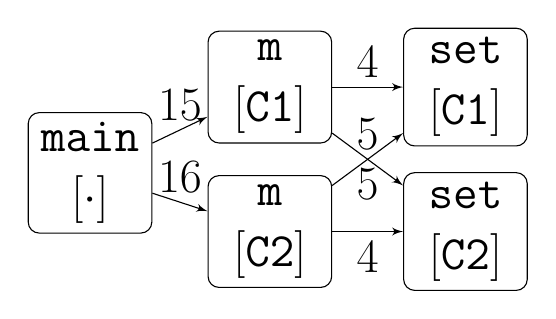
\begin{tikzpicture}
		\tikzstyle{every node}=[font=\LARGE]
		\node [block] (main) {{\tt main} \\ $[\cdot]$};
		\node [block, above right = -0.4cm and
		0.7cm of main] (Dm1) {\tt {m} \\$[$C1$]$};
		\node [block, below = 0.4cm of Dm1] (Dm2) {\tt{m} \\$[$C2$]$};
		\node [block, right = 0.9cm of Dm1] (Cm1) {\tt {set} \\$[$C1$]$};
		\node [block, right = 0.9cm of Dm2] (Cm2) {\tt {set} \\$[$C2$]$};
		
		\path [line] (main) edge node[above] {$15$} (Dm1);
		\path [line] (main) edge node[above] {$16$} (Dm2);
		\path [line] (Dm1) edge node[above] {$4$} (Cm1);
		\path [line] (Dm2) edge node[below] {$4$} (Cm2);
		\path [line] (Dm2) edge node[above] {$5$} (Cm1);
		\path [line] (Dm1) edge node[below] {$5$} (Cm2);
		
		\end{tikzpicture}
	}
\end{center}
\caption{Call-graph by 1-object sensitivity}
\label{fig:counterexample:obj}
\end{subfigure}~\\



\quad\begin{subfigure}[b]{1.0\columnwidth}

\begin{center}
	\resizebox{0.55\columnwidth}{!}{
		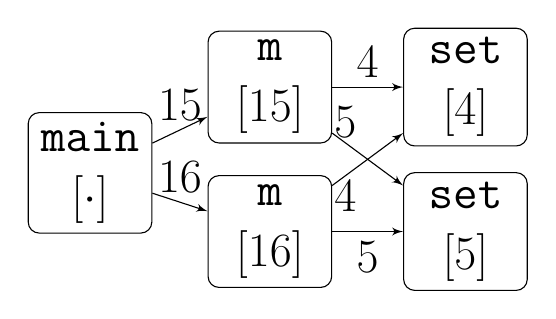
\begin{tikzpicture}
		\tikzstyle{every node}=[font=\LARGE]   
		\node [block] (main) {{\tt main} \\ $[\cdot]$};
		\node [block, above right = -0.4cm and
		0.7cm of main] (Dm1) {{\tt m} \\$[15]$};
		\node [block, below = 0.4cm of Dm1] (Dm2) {{\tt m} \\$[16]$};
		\node [block, right = 0.9cm of Dm1] (Cm1) {{\tt set} \\$[4]$};
		\node [block, right = 0.9cm of Dm2] (Cm2) {{\tt set} \\$[5]$};
		
		\path [line] (main) edge node[above] {$15$} (Dm1);
		\path [line] (main) edge node[above] {$16$} (Dm2);
		\path [line] (Dm1) edge node[above] {$4$} (Cm1);
		\path [line] (Dm2) edge node[below] {$5$} (Cm2);
		\path [line] (Dm2) edge node[above left= 0.15cm and 0.02cm] {$5$} (Cm1);
		\path [line] (Dm1) edge node[below left= 0.15cm and 0.02cm] {$4$} (Cm2);	
		\end{tikzpicture}
	}
\end{center}
\caption{Call-graph by 1-call-site sensitivity}
\label{fig:counterexample:call}
\end{subfigure}

\end{multicols}
\vspace{-15pt}
\caption{Example such that call-site sensitivity cannot
  simulate object sensitivity w.r.t. tunneling space $\mbs = \Invo$.}
\vspace{-10pt}
\label{fig:counterexample}
\end{figure}

First, we point out that that the condition (\ref{eq:sup-condition}) does not hold w.r.t. the tunneling space considered in this chapter. 
In Section~\ref{sec:setting}, we defined the tunneling space $\mbs$ to be the set of invocation-sites, i.e., $\mbs = \Invo$. 
With this space, there exists a tricky counter-example program that context-tunneled
call-site sensitivity is unable to simulate object sensitivity.
Consider the program in Figure~\ref{fig:counterexample}. 
In the example code, class {\tt C} contains two methods, {\tt set} and {\tt m}.
Method {\tt set} is a setter that stores the parameter value in the
the field of the base object,
and method {\tt m} calls the {\tt set} method twice
with the receiver object and parameter being swapped.
The {\tt main} method creates two objects, {\tt C1} and {\tt C2}, and
stores them in {\tt c1} and {\tt c2}. Method {\tt m} is called on {\tt
  c1} with parameter {\tt c2} at line 15, and it is called again on
{\tt c2} with parameter {\tt c1} at line 16.
At line 17, an assertion asks if
the fields of {\tt c1} and {\tt c2} are not aliased.
In the real execution, the query holds because {\tt c1.f} points to {\tt C2} and
{\tt c2.f} points to {\tt C1}.

The conventional 1-object-sensitive analysis can prove the query but
1-call-site sensitivity cannot do so no matter what tunneling abstraction from the space $\mbs = \Invo$ is
chosen.
Figure~\ref{fig:counterexample:obj} presents
the call-graph of 1-object sensitivity.
The object-sensitive analysis is effectively producing the call-graph above as
each context of {\tt set} determines the value of each parameter.
When the context is {\tt [C1]}, the receiver object is {\tt C1} and the value of the parameter is {\tt C2}.
Otherwise, when the context is {\tt [C2]}, the receiver object and the
parameter value are  {\tt C2} and {\tt C1}, respectively.
On the other hand, conventional 1-call-site sensitivity constructs a similar but
different call-graph in Figure~\ref{fig:counterexample:call}.
Note that the two edges labeled 4 go
to the same method but they are heading to different methods in the call-graph of object sensitivity. 
Thus, it is not possible to simulate object sensitivity with the invocation-site-based context tunneling. 
%However,
%doing so still fails to simulate object sensitivity.


%The code pattern, however, is uncommon in practice.
%To make call-site sensitivity unable to simulate object sensitivity,
%the program should have at least two invocation-sites where a single method
%is called with different parameters and receiver objects.
%The parameters should come from the parameters of the caller methods, and the
%caller method should be called from at least two different invocations with
%different parameters. Satisfying all of these constraints at the same time
%would happen rarely in practice.


%\textcolor{red}{
%\footnote{
%We can define the tunneling abstraction in various ways.
%\citet{JeJeOh18} originally used (pairs of) methods as tunneling abstractions.
%In this paper, we consider more fine-grained program elements, i.e., invocation-sites. 
%} 

\begin{figure}[t]
	\begin{center}
			\resizebox{0.8\columnwidth}{!}{
					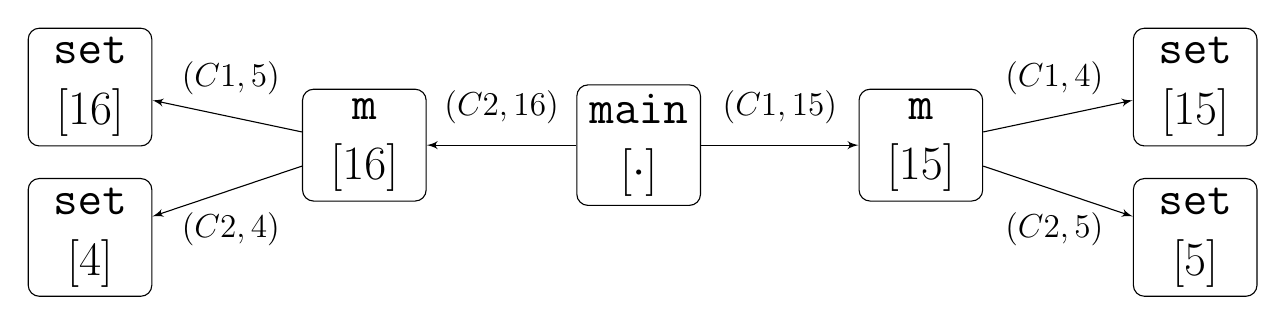
\begin{tikzpicture}
					\tikzstyle{every node}=[font=\LARGE]
					\node [block] (main) {{\tt main} \\ $[\cdot]$};
					\node [block, right =
					2.0cm of main] (Dm1) {{\tt m} \\$[15]$};
					\node [block, left = 1.9cm of main] (Dm2) {{\tt m} \\$[16]$};
					\node [block, below right = -0.3cm and 1.9cm of Dm1] (Cm1) {{\tt set} \\$[5]$};
					\node [block, below left = -0.3cm and 1.9cm of Dm2] (Cm2) {{\tt set} \\$[4]$};
	
					\node [block, above = 0.4cm of Cm1] (Cm3) {{\tt set} \\$[15]$};
					\node [block, above = 0.4cm of Cm2] (Cm4) {{\tt set} \\$[16]$};
	
	
					\path [line] (main) edge node[above= 0.15cm] {\large$(C1,15)$} (Dm1);
					\path [line] (main) edge node[above= 0.15cm] {\large$(C2,16)$} (Dm2);
					\path [line] (Dm1) edge node[above left= 0.15cm and -0.7cm] {\large $(C1,4)$} (Cm3);
					\path [line] (Dm2) edge node[above right= 0.15cm and -0.7cm] {\large $(C1,5)$} (Cm4);
					\path [line] (Dm2) edge node[below right = 0.15cm and -0.7cm] {\large $(C2,4)$} (Cm2);
					\path [line] (Dm1) edge node[below left = 0.15cm and -0.7cm] {\large $(C2,5)$} (Cm1);
					\end{tikzpicture}
			}
	\end{center}
	\caption{Call-graph with a fine-grained tunneling space}
	\label{fig:cg-finegrained}
	\vspace{-10pt}
	\end{figure}
However, this counter-example does not mean that it is fundamentally impossible to simulate object sensitivity via call-site sensitivity, as the counter-example becomes no longer valid if we use a more fine-grained tunneling abstraction. 
For example, suppose we define the tunneling space to be pairs of receiver objects and invocation-sites, i.e., $\mbs = \Heap \times \Invo$ (recall that choosing a tunneling abstraction does not affect the analysis soundness). 
With this tunneling space, a context-tunneled 1-call-site-sensitive analysis can now prove the query. 
Suppose we use a tunneling abstraction $T = \myset{(C1,4), (C1,5)}$, which means that we apply context tunneling only when the receiver object is $C1$ and the invocation-site is either $4$ or $5$. 1-call-site sensitivity with $T$ produces the call-graph in Figure~\ref{fig:cg-finegrained}. 
In the call-graph, $\texttt{m[15]} \stackrel{(C1,4)}{\to}
\texttt{set[15]}$ indicates that the caller ({\tt m}) and callee ({\tt
  set}) have the same context 15 where the callee method is called at
invocation-site 4 and its receiver object is $C1$. With this call-graph, we can prove the query 
in Figure~\ref{fig:counterexample:code} as it is strictly more precise than the call-graph produced by object sensitivity
(Figure~\ref{fig:counterexample:obj}). 



%Note that the above counter-example is not valid that 1-call-site
%sensitivity with tunneling can prove the query if we use a generalized
%abstraction space of context tunneling instead of invocation sites. if
%we use pairs of receiver objects and invocation sites as tunneling
%abstraction, 1-call-site-sensitive analysis with tunneling can prove
%the query in the example
%(Figure~\ref{fig:counterexample:call}). Suppose we use a
%tunneling abstraction $T = \{(C1,4),(C1,5)\}$ where it applied context
%tunneling when the receiver object and invocation site are $C1$ and
%$4$, respectively, or the object and the invocation site are $C2$
%and $5$, respectively. It produces
%the following context abstraction:



This way, we conjecture that it would be always possible to find a suitable context-tunneling space $\mbs$ that satisfies the condition (\ref{eq:sup-condition}) w.r.t. the given set of programs ($\mbp$). We leave an in-depth theoretical analysis as future work. 

%}




%%% Local Variables:
%%% mode: latex
%%% TeX-master: "paper"
%%% End:

%


%the high-level idea of our approach could be adapted for m-CFA and we think it will be an interesting direction for extending our work.
%Our current simulation technique relies on specific properties of k-CFA (e.g., I_2I 2​	
%leverages a unique property of context-tunneled k-CFA). Therefore applying our technique as it is may not be effective for m-CFA [2]. 

% !TEX root = ./paper.tex

\section{Conclusion and Future Work}

Unfortunately, the program analysis community for object-oriented programs has dismissed call-site sensitivity for a long time. 
In this paper, 
showed that 
call-site sensitivity has vast untapped potential, even more than object sensitivity, when the notion of $k$-limiting is generalized. We provided an insight that call-site sensitivity with context tunneling can simulate object sensitivity and experimentally proved that the observation holds in practice by developing a technique to transform a baseline object-sensitive analysis into more precise, context-tunneled call-site sensitivity. 
Based on our results, we hope that the community reconsiders call-site sensitivity from now on.  


%We demonstrated that our technique enables call-site sensitivity to outperform modern object-sensitive analyses for real-world Java programs in both precision and cost.

%when designing context-sensitive analyses.


Many problems remain as future work. We already discussed a theoretical issue in Section~\ref{sec:counter_example}. 
Other problems include the following. 


\begin{itemize}

\item {\em Can we learn better tunneling strategies than just simulating object sensitivity?} 
Our goal in this paper was to show that call-site sensitivity can be superior to object sensitivity, and simulating object sensitivity was an effective means of achieving this goal. 
However, simulating object sensitivity would be a suboptimal strategy for call-site sensitivity; 
we believe an optimal tunneling strategy would enable call-site sensitivity to show far better precision than ours (\ours).
Thus, an interesting direction for future work is to develop a powerful learning algorithm to find such strategies, where 
the main challenge is how to efficiently explore the huge and non-monotone tunneling space~\cite{JeJeOh18}. Using reinforcement learning, for example, could be a promising approach to address this challenge. 

%in the huge and non-monotone tunneling space~\cite{JeJeOh18}. 
%For example, reinforcement learning could be a promising approach to address this challenge.

\item {\em Can our approach be adapted for other flavors of context-sensitive analyses?}
Our current simulation technique relies on properties specific to $k$-CFA (e.g., $I_2$ in Section~\ref{sec:simulation} leverages a unique property of context-tunneled $k$-CFA). However, the high-level idea (i.e., simulating object sensitivity) would be applicable to other analyses. 
For example, it would be interesting if our idea could be adapted for $m$-CFA~\cite{Might10}. 
% by leveraging properties of context-tunneled $m$-CFA. 



% instead of k-CFA with your technique would produce better, similar, or worse results.


% High-level idea of our approach (simulating object sensitivity) is applicable to other contexts. 
%Directly applying our technique may not effective as
%it relies on specific properties of k-CFA (e.g., $I_2$ leverages a unique property of context-tunneled k-CFA).
%However, the high-level idea of our approach could be adapted.
%For example, applying our approach could be adapted for m-CFA~\cite{Might10} by leveraging properties of context tunneled m-CFA.

\end{itemize}






% \myparagraph{Future Work}

% \begin{itemize}

% \item {\bf Better context tunneling for call-site-sensitivity}:

% \item {\bf General technique for simulation}:  Our simulation technique was designed to work on the
%   call-graph produced by an object-sensitive analysis. Therefore, the
%   resulting call-site-sensitive analysis is likely to be effective for
%   type-dependent clients (e.g. may-fail casts).

%\end{itemize}

%%% Local Variables:
%%% mode: latex
%%% TeX-master: "paper"
%%% End:


\begin{acks}
We thank the anonymous POPL reviewers for their constructive feedback. 
This work was supported by Samsung Research Funding \& Incubation Center of Samsung Electronics under Project Number SRFC-IT1701-51. 
This work was partly supported by 
Institute of Information \& communications Technology Planning \& Evaluation (IITP) grant funded by the Korea government(MSIT) (No.2020-0-01337, (SW STAR LAB) Research on Highly-Practical Automated Software Repair) 
and by the MSIT(Ministry of Science and ICT), Korea, under the ICT Creative Consilience program(IITP-2021-2020-0-01819) supervised by the IITP(Institute for Information \& communications Technology Planning \& Evaluation), and by the National Research Foundation of Korea(NRF) grant funded by the Korea government(MSIT)(No. 2021R1A5A1021944).







\end{acks}


%% Bibliography
\bibliography{refs}

%% Appendix
%%\section{Notations}\label{sec:max}
%The function $\MaxIn(G_\vec{P})$ returns the maximum number $max\in\mbn$ of
%incoming edges of a node in the graphs that $max$ satisfies:
%%\[
%%\begin{array}{c}
%\begin{enumerate}
%\item %There exists a node $n$ that have $max$ incoming edges:\\
%$max$ is a node's incoming edges:
%$\exists P\in\vec{P}. (N,E) =
%  G_\vec{P}(P) \land \exists n\in N. |\{n' \mid (n',n)\in E\}| = max$
%\item The node has equal or more number of
%incomingedges than the others: \\
%$\forall P \in \vec{P}. (N,E) = G_\vec{P}(P) \land \forall n\in N. |\{n' \mid (n',n)\in E
%\}| \le max$
%\end{enumerate}
%%\end{array}
%%\]
%On the other hand, $\MaxOut(G_\vec{P})$ returns the maximum number $max\in\mbn$ of
%outgoing edge of a node in the graphs:
%\begin{enumerate}
%\item $max$ is a node's outgoing edges: $\exists P\in\vec{P}. (N,E) = G_\vec{P}(P) \land \exists n\in N. |\{n' \mid (n,n')\in E
%\}| = max$
%\item The node has equal or more number of
%incomingedges than the others: \\
%$\forall P \in \vec{P}. (N,E) = G_\vec{P}(P) \land \forall n\in N. |\{n' \mid (n,n')\in E
%\}| \le max$
%\end{enumerate}

% \[
% Incoming(n,G) = |\{n' \mid (n',n)\in E \land G = (N,E) \}|
% \]
% \[
% Outgoing(n,G) = |\{n' \mid (n,n')\in E \land G = (N,E) \}|
% \]
% \[
% \forall n \in G' \in G_\vec{P}. Incoming(n,G) \ge Incoming(n',G')
% \]
% where $Incoming$ returns the number of incoming edges for each node:
% \[
% Incoming(n,G) = |\{n' \mid (n',n)\in E \land G = (N,E) \}|
% \]
% On the other hand, $\MaxOut(G_\vec{P})$ returns the maximul number of incoming edges
% of a node $n$ in the graphs:
% \[
% \forall n \in G_\vec{P}. Incoming(n,G) \ge Incoming(n',G')
% \]
% where $Outgoing$ returns the number of the node's outgoing edges:
% \[
% Outgoing(n,G) = |\{n' \mid (n,n')\in E \land G = (N,E) \}|
% \]



\chapter{Proof of Theorem~\ref{THM:REDUCESPACE}}\label{sec:proof}

%{\textsc LearningMinimalAbstraction}\label{alg:Learnminimal}

We will show that the output of Algorithm~\ref{alg:Learnminimal} in Section~\ref{sec:learning-algorithm} is the minimal abstraction of the given program using proof by induction and contradiction.
Let $\abs$ be the output of the learning algorithm.  
$\abs$ is a precise abstraction because our algorithm updates $\abs$ only if the following equation holds:
\[
\projproved(F_P(\abs)) = \projproved(F_P(\absk)).
\]
Assume that $\abs'$ meets the precision constraint but smaller than $\abs$:
\begin{equation}\label{eq:assumption}
\projproved(F_P(\abs')) = \projproved(F_P(\absk)) \land
\abs' \sqsubseteq \abs.
\end{equation}
We can prove that $\abs$ is the minimal abstraction by showing that $\abs'$ equals to $\abs$:
%It suffices to show that:
\begin{equation}\label{eq:goal}
\forall i \in [0,k].\{c \mid c \in \component_P \land \abs(c) = i\} = \{c \mid c\in \component_P \land \abs'(c) = i\}.
\end{equation}
We prove~(\ref{eq:goal}) with induction on $i$ in decreasing order.
\begin{itemize}
\item (Base case) the base case is as follows:
\begin{equation}\label{eq:base:goal}
\{c \mid c\in \component_P \land \abs(c) = k\} = \{c \mid c\in \component_P \land \abs'(c) = k\}.
\end{equation}
From~(\ref{eq:assumption}), we have
\begin{equation}\label{eq:base:obvious}
\emptyset = \{c \mid c\in \component_P \land \abs'(c) = k\} \setminus \{c \mid c\in \component_P \land \abs(c) = k\}.
\end{equation}
Now, we can prove~(\ref{eq:base:goal}) by showing the following counterpart is also $\emptyset$ by the proof of contradiction:
\begin{equation}\label{eq:base:counter}
\{c \mid c\in \component_P \land \abs(c) = k\} \setminus \{c \mid c\in \component_P \land \abs'(c) = k\}.
\end{equation}
Assume that~(\ref{eq:base:counter}) is not an empty set, then it has a program component $c'$:
\[
c' \in (\{c \mid c\in \component_P \land \abs(c) = k\} \setminus \{c \mid c\in \component_P \land \abs'(c) = k\}).
\]
%Let $\abs''$ be the abstraction when $c'$ was considered in the first iteration.
Let $\abs''$ be the abstraction when $c'$ is chosen.
Then, we have
\begin{equation}\label{eq:base:small}
 \abs'\sqsubseteq \abs''.
\end{equation}
The abstraction $\abs''$ is less precise than $\vec{k}$:
%not precise enough as $c'$ is rejected:
\begin{equation}\label{eq:base:notprecise}
\projproved(F_P(\abs''))<\projproved(F_P(\absk)).
\end{equation}
From~(\ref{eq:assumption}),~(\ref{eq:base:small}), and the monotonicity of analysis, we have
\begin{equation}\label{eq:base:precise}
\projproved(F_P(\absk)) = \projproved(F_P(\abs')) \le \projproved(F_P(\abs'')).
\end{equation}
Now, we have a contradiction between~(\ref{eq:base:notprecise}) and~(\ref{eq:base:precise}).
As a result, we have:
\begin{equation}\label{eq:base:Notobvious}
\emptyset = (\{c \mid c\in \component_P \land \abs(c) = k\} \setminus \{c \mid c\in \component_P \land \abs'(c) = k\}).
\end{equation}
From~(\ref{eq:base:obvious}) and~(\ref{eq:base:Notobvious}), we prove the base case~(\ref{eq:base:goal}) is true.\\

\item (Inductive case) 
The induction hypothesis is as follows:
\begin{equation}\label{eq:ind:hypo}
\forall j \in [l,k].\{c \mid c \in \component_P \land \abs(c) = j\} = \{c \mid c \in \component_P \land \abs'(c) = j\}
\end{equation}
where $2\le l\le k$.
From the hypothesis, we will prove that the following equation is true:
\begin{equation}\label{eq:ind:goal}
\{c \mid c \in \component_P \land \abs(c) = l-1\} = \{c \mid c\in \component_P \land \abs'(c) = l-1\}.
\end{equation}
From~(\ref{eq:assumption}) and~(\ref{eq:ind:hypo}), we have
\begin{equation}\label{eq:ind:obvious}
\emptyset = \{c \mid c\in \component_P \land \abs'(c) = l-1\} \setminus \{c \mid c\in \component_P \land \abs(c) = l-1\}.
\end{equation}
Now, we will show the following counterpart is also $\emptyset$ by the proof of contradiction:
\begin{equation}\label{eq:ind:counter}
\{c \mid c\in \component_P \land \abs(c) = l-1\} \setminus \{c \mid c\in \component_P \land \abs'(c) = l-1\}.
\end{equation}
Assume that (\ref{eq:ind:counter}) has a program component $c''$.
Let $\abs'''$ be the abstraction when $c''$ is considered where $i$ equals to $l-1$ in the Algorithm~\ref{alg:Learnminimal}. From~(\ref{eq:ind:hypo}), we can get the following relation between $\abs'$ and $\abs'''$:
\begin{equation}\label{eq:ind:small}
\abs'\sqsubseteq \abs'''.
\end{equation}
$\abs'''$ is less precise than $\vec{k}$:
%not precise enough as $c'$ is rejected:
\begin{equation}\label{eq:ind:notprecise}
\projproved(F_P(\abs'''))<\projproved(F_P(\absk)).
\end{equation}
From~(\ref{eq:assumption}),~(\ref{eq:ind:small}), and the monotonicity of analysis, we have
\begin{equation}\label{eq:ind:precise}
\projproved(F_P(\absk)) = \projproved(F_P(\abs')) \le \projproved(F_P(\abs''')).
\end{equation}
We also find a contradiction between~(\ref{eq:ind:notprecise}) and~(\ref{eq:ind:precise}).
Now, we have
\begin{equation}\label{eq:ind:Notobvious}
\emptyset = (\{c \mid c\in \component_P \land \abs(c) = l-1\} \setminus \{c \mid c\in \component_P \land \abs'(c) = l-1\}).
\end{equation}
From~(\ref{eq:ind:obvious}) and~(\ref{eq:ind:Notobvious}), we can prove the following equation is true:
\[
\{c \mid c\in \component_P \land a_P(c) = l-1\} = \{c \mid c\in \component_P \land a_P'(c) = l-1\}.
\]

\end{itemize}


%%% Local Variables:
%%% mode: latex
%%% TeX-master: "paper"
%%% End:

%\appendix
%%\section{Notations}\label{sec:max}
%The function $\MaxIn(G_\vec{P})$ returns the maximum number $max\in\mbn$ of
%incoming edges of a node in the graphs that $max$ satisfies:
%%\[
%%\begin{array}{c}
%\begin{enumerate}
%\item %There exists a node $n$ that have $max$ incoming edges:\\
%$max$ is a node's incoming edges:
%$\exists P\in\vec{P}. (N,E) =
%  G_\vec{P}(P) \land \exists n\in N. |\{n' \mid (n',n)\in E\}| = max$
%\item The node has equal or more number of
%incomingedges than the others: \\
%$\forall P \in \vec{P}. (N,E) = G_\vec{P}(P) \land \forall n\in N. |\{n' \mid (n',n)\in E
%\}| \le max$
%\end{enumerate}
%%\end{array}
%%\]
%On the other hand, $\MaxOut(G_\vec{P})$ returns the maximum number $max\in\mbn$ of
%outgoing edge of a node in the graphs:
%\begin{enumerate}
%\item $max$ is a node's outgoing edges: $\exists P\in\vec{P}. (N,E) = G_\vec{P}(P) \land \exists n\in N. |\{n' \mid (n,n')\in E
%\}| = max$
%\item The node has equal or more number of
%incomingedges than the others: \\
%$\forall P \in \vec{P}. (N,E) = G_\vec{P}(P) \land \forall n\in N. |\{n' \mid (n,n')\in E
%\}| \le max$
%\end{enumerate}

% \[
% Incoming(n,G) = |\{n' \mid (n',n)\in E \land G = (N,E) \}|
% \]
% \[
% Outgoing(n,G) = |\{n' \mid (n,n')\in E \land G = (N,E) \}|
% \]
% \[
% \forall n \in G' \in G_\vec{P}. Incoming(n,G) \ge Incoming(n',G')
% \]
% where $Incoming$ returns the number of incoming edges for each node:
% \[
% Incoming(n,G) = |\{n' \mid (n',n)\in E \land G = (N,E) \}|
% \]
% On the other hand, $\MaxOut(G_\vec{P})$ returns the maximul number of incoming edges
% of a node $n$ in the graphs:
% \[
% \forall n \in G_\vec{P}. Incoming(n,G) \ge Incoming(n',G')
% \]
% where $Outgoing$ returns the number of the node's outgoing edges:
% \[
% Outgoing(n,G) = |\{n' \mid (n,n')\in E \land G = (N,E) \}|
% \]



\chapter{Proof of Theorem~\ref{THM:REDUCESPACE}}\label{sec:proof}

%{\textsc LearningMinimalAbstraction}\label{alg:Learnminimal}

We will show that the output of Algorithm~\ref{alg:Learnminimal} in Section~\ref{sec:learning-algorithm} is the minimal abstraction of the given program using proof by induction and contradiction.
Let $\abs$ be the output of the learning algorithm.  
$\abs$ is a precise abstraction because our algorithm updates $\abs$ only if the following equation holds:
\[
\projproved(F_P(\abs)) = \projproved(F_P(\absk)).
\]
Assume that $\abs'$ meets the precision constraint but smaller than $\abs$:
\begin{equation}\label{eq:assumption}
\projproved(F_P(\abs')) = \projproved(F_P(\absk)) \land
\abs' \sqsubseteq \abs.
\end{equation}
We can prove that $\abs$ is the minimal abstraction by showing that $\abs'$ equals to $\abs$:
%It suffices to show that:
\begin{equation}\label{eq:goal}
\forall i \in [0,k].\{c \mid c \in \component_P \land \abs(c) = i\} = \{c \mid c\in \component_P \land \abs'(c) = i\}.
\end{equation}
We prove~(\ref{eq:goal}) with induction on $i$ in decreasing order.
\begin{itemize}
\item (Base case) the base case is as follows:
\begin{equation}\label{eq:base:goal}
\{c \mid c\in \component_P \land \abs(c) = k\} = \{c \mid c\in \component_P \land \abs'(c) = k\}.
\end{equation}
From~(\ref{eq:assumption}), we have
\begin{equation}\label{eq:base:obvious}
\emptyset = \{c \mid c\in \component_P \land \abs'(c) = k\} \setminus \{c \mid c\in \component_P \land \abs(c) = k\}.
\end{equation}
Now, we can prove~(\ref{eq:base:goal}) by showing the following counterpart is also $\emptyset$ by the proof of contradiction:
\begin{equation}\label{eq:base:counter}
\{c \mid c\in \component_P \land \abs(c) = k\} \setminus \{c \mid c\in \component_P \land \abs'(c) = k\}.
\end{equation}
Assume that~(\ref{eq:base:counter}) is not an empty set, then it has a program component $c'$:
\[
c' \in (\{c \mid c\in \component_P \land \abs(c) = k\} \setminus \{c \mid c\in \component_P \land \abs'(c) = k\}).
\]
%Let $\abs''$ be the abstraction when $c'$ was considered in the first iteration.
Let $\abs''$ be the abstraction when $c'$ is chosen.
Then, we have
\begin{equation}\label{eq:base:small}
 \abs'\sqsubseteq \abs''.
\end{equation}
The abstraction $\abs''$ is less precise than $\vec{k}$:
%not precise enough as $c'$ is rejected:
\begin{equation}\label{eq:base:notprecise}
\projproved(F_P(\abs''))<\projproved(F_P(\absk)).
\end{equation}
From~(\ref{eq:assumption}),~(\ref{eq:base:small}), and the monotonicity of analysis, we have
\begin{equation}\label{eq:base:precise}
\projproved(F_P(\absk)) = \projproved(F_P(\abs')) \le \projproved(F_P(\abs'')).
\end{equation}
Now, we have a contradiction between~(\ref{eq:base:notprecise}) and~(\ref{eq:base:precise}).
As a result, we have:
\begin{equation}\label{eq:base:Notobvious}
\emptyset = (\{c \mid c\in \component_P \land \abs(c) = k\} \setminus \{c \mid c\in \component_P \land \abs'(c) = k\}).
\end{equation}
From~(\ref{eq:base:obvious}) and~(\ref{eq:base:Notobvious}), we prove the base case~(\ref{eq:base:goal}) is true.\\

\item (Inductive case) 
The induction hypothesis is as follows:
\begin{equation}\label{eq:ind:hypo}
\forall j \in [l,k].\{c \mid c \in \component_P \land \abs(c) = j\} = \{c \mid c \in \component_P \land \abs'(c) = j\}
\end{equation}
where $2\le l\le k$.
From the hypothesis, we will prove that the following equation is true:
\begin{equation}\label{eq:ind:goal}
\{c \mid c \in \component_P \land \abs(c) = l-1\} = \{c \mid c\in \component_P \land \abs'(c) = l-1\}.
\end{equation}
From~(\ref{eq:assumption}) and~(\ref{eq:ind:hypo}), we have
\begin{equation}\label{eq:ind:obvious}
\emptyset = \{c \mid c\in \component_P \land \abs'(c) = l-1\} \setminus \{c \mid c\in \component_P \land \abs(c) = l-1\}.
\end{equation}
Now, we will show the following counterpart is also $\emptyset$ by the proof of contradiction:
\begin{equation}\label{eq:ind:counter}
\{c \mid c\in \component_P \land \abs(c) = l-1\} \setminus \{c \mid c\in \component_P \land \abs'(c) = l-1\}.
\end{equation}
Assume that (\ref{eq:ind:counter}) has a program component $c''$.
Let $\abs'''$ be the abstraction when $c''$ is considered where $i$ equals to $l-1$ in the Algorithm~\ref{alg:Learnminimal}. From~(\ref{eq:ind:hypo}), we can get the following relation between $\abs'$ and $\abs'''$:
\begin{equation}\label{eq:ind:small}
\abs'\sqsubseteq \abs'''.
\end{equation}
$\abs'''$ is less precise than $\vec{k}$:
%not precise enough as $c'$ is rejected:
\begin{equation}\label{eq:ind:notprecise}
\projproved(F_P(\abs'''))<\projproved(F_P(\absk)).
\end{equation}
From~(\ref{eq:assumption}),~(\ref{eq:ind:small}), and the monotonicity of analysis, we have
\begin{equation}\label{eq:ind:precise}
\projproved(F_P(\absk)) = \projproved(F_P(\abs')) \le \projproved(F_P(\abs''')).
\end{equation}
We also find a contradiction between~(\ref{eq:ind:notprecise}) and~(\ref{eq:ind:precise}).
Now, we have
\begin{equation}\label{eq:ind:Notobvious}
\emptyset = (\{c \mid c\in \component_P \land \abs(c) = l-1\} \setminus \{c \mid c\in \component_P \land \abs'(c) = l-1\}).
\end{equation}
From~(\ref{eq:ind:obvious}) and~(\ref{eq:ind:Notobvious}), we can prove the following equation is true:
\[
\{c \mid c\in \component_P \land a_P(c) = l-1\} = \{c \mid c\in \component_P \land a_P'(c) = l-1\}.
\]

\end{itemize}


%%% Local Variables:
%%% mode: latex
%%% TeX-master: "paper"
%%% End:

%% !TEX root = ./paper.tex
\clearpage
\newtheorem{openquestion}{Question}

\section{Open Question: Is Complete Simulation Possible?}

\subsection{High Level Description}

The observation in Section~\ref{sec:counter_example}, that there exists
a counter-example in our setting (tunneling abstraction space is a set
of invocation site) but the counter-example is not the case in a more
generalized abstraction space of context tunneling (pairs of
invocation and receiver object), lead us to the following open question.
%\begin{equation}
\begin{openquestion}\label{openQ}
Can we define a tunneling abstraction space $S$ (e.g., pairs of receiver
object and invocation site) that $k$-call-site sensitivity with
tunneling can always become equal or more precise than $k$-object
sensitivity with tunneling?
\end{openquestion}
%\end{equation}
If the above question is true (we can define such tunneling
abstraction space), $k$-call-site sensitivity is theoretically more
precise than $k$-object sensitivity when k-limited context sensitivity
is generalized with context tunneling. The formal description of the
open question is described in Section~\ref{sec:quextion:formal}. 

% (in flow-insensitive but context sensitive pointer analysis)

Note that the converse is not true; it is unable to define a tunneling
abstraction space $S$ that $k$-object sensitivity with
tunneling can always become equal or more precise than $k$-call-site
sensitivity with tunneling. The example code in
Figure~\ref{background:example2} is a counter-example for an arbitrary
tunneling abstraction space. By the definition of context tunneling
(determine whether to update context or not), the method
{\tt id} in the example (Figure~\ref{background:example2}) can have
the the contexts \texttt{[D]} (update context) or \texttt{[$\cdot$]}
(inherit context) no matter what tunneling abstraction space is
used. $k$-object sensitivity with tunneling is unable to separate the
three method calls (invoked at the three different invocation sites)
with the two 
available contexts. k-call-site sensitivity, however, can separate the
three method calls with a tunneling abstraction $\emptyset \subseteq
S$ (always update contexts) for all tunneling abstraction space
$S$ of context tunneling. 


In this paper, we showed a set of invocation sites is practically (not
theoretically) the abstraction space ($T \subseteq \Invo$) that
k-call-site sensitivity with tunneling can simulate k-object
sensitivity with tunneling. Our future work 
is answering the {\sc Question~\ref{openQ}} to show that
call-site sensitivity is theoretically more precise than
object-sensitivity (the answer of the question is ``yes'') or the two
contexts are still incomparable in the generalized k-limited context
sensitivity (the answer is ``no''). 

%What we show in our paper is that invocation sites 




\subsection{Formal Description}~\label{sec:quextion:formal}
Let $F_{P,k}^{T, \updatectx}$ be the analysis uses the context update
function $\updatectx$, context depth $k\in\mbn$, tunneling abstraction
$T \subseteq S$ for analyzing the program $P$:
\begin{equation}\label{eq:analysis}
F_{P,k}^{T, \updatectx}(\ptsto, \reachable, \callgraph) = \bigsqcup_{\inst \in \Inst_P}
f_{k, \inst}^{T, \updatectx}(\ptsto,
\reachable, \callgraph)
\end{equation}
where $f_{k, \inst}^{T, \updatectx}$ is the transfer function (simply described
as $f_l$ in Section~\ref{sec:setting}) encoding
the abstract semantics of instructions. Running the analysis is to compute the least fixed point of
$F^{T, \updatectx}_{P,k}$:
\begin{equation}\label{eq:fixpoint}
  \fix F_{P,k}^{T, \updatectx} = F^{T, \updatectx}_{P,k}
  (\bot_\ptsto, \bot_\reachable,\bot_\callgraph) \sqcup F^{T, \updatectx}_{P,k}  (F^{T, \updatectx}_{P,k}
  (\bot_\ptsto, \bot_\reachable,\bot_\callgraph)) \sqcup \cdots
\end{equation}
where we define the bottom elements for the domains as follows:
\[
  \bot_\ptsto = \lambda (x,c).\emptyset, \qquad \bot_\reachable =
\lambda m. \left\{ \begin{array}{ll} \myset{\epsilon} & \mbox{if}~m =
                                                        \entry_P \\
                     \emptyset & \mbox{otherwise} \end{array} \right., \qquad
  \bot_\callgraph = \emptyset,
\]
%Note that the reachability map ($\reachable$) initially
%associates the entry method with the initial context
%$\epsilon$. 
The fixed point computation in (\ref{eq:fixpoint})
eventually stabilizes because the domains are
finite and the transfer function is monotone.




\myparagraph{Order of Analysis Precision}
 For two analyses $F_{P,k}^{T, \updatectx}$ and
 $F_{P,k'}^{T',\updatectx'}$ for program $P$, we say the former is more
 precise than (or equal to) the
 latter, denoted $F_{P,k}^{T, \updatectx} \moreprecise F_{P,k'}^{T', \updatectx'}$, if and only if
 \[
   \project(\fix F_{P,k}^{T, \updatectx}) \sqsubseteq \project(\fix F_{P,k'}^{T', \updatectx'})
 \]
 where $\project$ extracts the context-insensitive points-to
 information from the analysis result $(\ptsto, \reachable,\callgraph)$:
 \begin{equation}\label{eq:project}
 \project(X, R,\callgraph) = \lambda x.\; \bigsqcup_{\ctx \in \Ctx}
 \myset{h \mid (h, \hctx) \in X(x, \ctx)},
 \end{equation}
and the order between the two projected analysis results is defined as follows:
 \[
   \project(\fix F_{P,k}^{T, \updatectx}) \sqsubseteq \project(\fix
   F_{P,k'}^{T', \updatectx'}) \iff \forall x\in \Var_P. \project(\fix
   F_{P,k}^{T, \updatectx})(x) \subseteq \project(\fix
   F_{P,k'}^{T', \updatectx'}) (x).
 \]
That is, an analysis is more precise than the other if it produces
a strictly smaller points-to set for all variables.


Now we formalize the open question. 
Answering ``yes'' to the {\sc Question~\ref{openQ}} equals to show that the
following proposition holds:
\newtheorem{prop}{Proposition}
\begin{prop}
Let $\updatectx_{\it obj}$
and $\updatectx_{\it call}$ be the context functions for
object-sensitivity and call-site-sensitivity given in
(\ref{eq:objsens}) and (\ref{eq:cfa}), respectively. 
\begin{equation}\label{eq:conjecture}
\exists S. \; \forall P. \; \forall k\in \mbn. \; \forall T_{\it obj}\in S. \; \exists
T_{\it call} \in S. \; 
F_{P,k}^{T_{\it call},\updatectx_{{\it call}}}
\moreprecise F_{P,k}^{T_{\it obj}, \updatectx_{{\it obj}}}.
\end{equation}
\label{conjecture}
\end{prop}
That is, we can define a tunneling abstraction space $S$ that
for a given program $P$, context depth $k$, and tunneling abstracion for
object sensitivity $T_{\it obj} \in S$, we can find a
corresponding tunenling abstraction for call-site sensitivity $T_{\it
  call} \in S$ that make $k$-call-site sensitivity with tunneling
($F_{P,k}^{T_{\it call},\updatectx_{{\it call}}}$) produce a more
precise analysis result than the
given object sensitivity with tunneling ($F_{P,k}^{T_{\it obj},
  \updatectx_{{\it obj}}}$).
If there is no such abstraction space (the answer to {\sc
  Question~\ref{openQ}} is ``no''), call-site sensitivity and 
object sensitivity are still incomparable in the generalized
k-limited context sensitivity
(we already showed it is unable to define a
tunneling space that 
object sensitivity with tunneling can always become equal or more
precise than call-site sensitivity). 


%%% Local Variables:
%%% mode: latex
%%% TeX-master: "paper"
%%% End:


% Please add the following required packages to your document preamble:
% \usepackage{multirow}
\end{document}
